%%
%% This is file `ubcsample.tex',
%% generated with the docstrip utility.
%
% The original source files were:
%
% ubcthesis.dtx  (with options: `ubcsampletex')
%% 
%% This file was generated from the ubcthesis package.
%% --------------------------------------------------------------
%% 
%% Copyright (C) 2001
%% Michael McNeil Forbes
%% mforbes@alum.mit.edu
%% 
%% This file may be distributed and/or modified under the
%% conditions of the LaTeX Project Public License, either version 1.2
%% of this license or (at your option) any later version.
%% The latest version of this license is in
%%    http://www.latex-project.org/lppl.txt
%% and version 1.2 or later is part of all distributions of LaTeX
%% version 1999/12/01 or later.
%% 
%% This program is distributed in the hope that it will be useful,
%% but WITHOUT ANY WARRANTY; without even the implied warranty of
%% MERCHANTABILITY or FITNESS FOR A PARTICULAR PURPOSE.  See the
%% LaTeX Project Public License for more details.
%% 
%% This program consists of the files ubcthesis.dtx, ubcthesis.ins, and
%% the sample figures fig.eps and fig.fig.
%% 
%% This file may be modified and used as a base for your thesis without
%% including the licence agreement as long as the content (i.e. textual
%% body) of the file is completely rewritten. You must, however, change
%% the name of the file.
%% 
%% This file may only be distributed together with a copy of this
%% program. You may, however, distribute this program without generated
%% files such as this one.
%% 

% This Sample thesis requires \LaTeX2e
\NeedsTeXFormat{LaTeX2e}[1995/12/01]
% \ProvidesFile{ubcsample.tex}[2015/05/31 v1.72 ^^J
%  University of British Columbia Sample Thesis]

% This is the \documentclass[]{} command.  The manditory argument
% specifies the "flavour" of thesis (ubcthesis for UBC).  The
% optional arguments (in []) specify options that affect how the
% thesis is displayed.  Please see the ubcthesis documentation for
% details about the options.
\documentclass[msc,oneside,noheadline, draft]{ubcthesis} 
% draft
% REMOVE4HANDIN: remove draft 
%
% To compile this sample thesis, issue the following commands:
% latex ubcsample
% bibtex ubcsample
% latex ubcsample

%
% To view use xdvi (on unix systems):
% xdvi ubcsample.dvi
%
% To make a postscript file, use dvips:
% dvips -o ubcsample.ps ubcsample.dvi
%
% To view the postscript file, use ghostview or gv (on unix systems):
% gv ubcsample.ps
%
%************************************************
% Optional packages.
%
% The use of these packages is optional, but they provide various
% tools for more flexible formating.  The sample thesis uses these,
% but if you remove the example code, you should be able to exclude
% these packages.  Only standard packages have been described here;
% they should be installed with any complete LaTeX instalation, but
% if not, you can find them at the Comprehensive TeX Archive Network
% (CTAN): http://www.ctan.org/
%

%******** afterpage ***************************
% This package allows you to issue commands at the end of the current
% page.  A good use for this is to use the command
% \afterpage{\clearpage} right after a figure.  This will cause the
% figure to be inserted on the page following the current one (or on
% the current page if it will fit) but will not break the page in the
% middle.
\usepackage{afterpage}


\usepackage{epigraph,varwidth}

\renewcommand{\epigraphsize}{\small}
\setlength{\epigraphwidth}{0.8\textwidth}
\renewcommand{\textflush}{flushright}
\renewcommand{\sourceflush}{flushright}
% A useful addition
\newcommand{\epitextfont}{\itshape}
\newcommand{\episourcefont}{\scshape}

\makeatletter
\newsavebox{\epi@textbox}
\newsavebox{\epi@sourcebox}
\newlength\epi@finalwidth
\renewcommand{\epigraph}[2]{%
  \vspace{\beforeepigraphskip}
  {\epigraphsize\begin{\epigraphflush}
   \epi@finalwidth=\z@
   \sbox\epi@textbox{%
     \varwidth{\epigraphwidth}
     \begin{\textflush}\epitextfont#1\end{\textflush}
     \endvarwidth
   }%
   \epi@finalwidth=\wd\epi@textbox
   \sbox\epi@sourcebox{%
     \varwidth{\epigraphwidth}
     \begin{\sourceflush}\episourcefont#2\end{\sourceflush}%
     \endvarwidth
   }%
   \ifdim\wd\epi@sourcebox>\epi@finalwidth 
     \epi@finalwidth=\wd\epi@sourcebox
   \fi
   \leavevmode\vbox{
     \hb@xt@\epi@finalwidth{\hfil\box\epi@textbox}
     \vskip1.75ex
     \hrule height \epigraphrule
     \vskip.75ex
     \hb@xt@\epi@finalwidth{\hfil\box\epi@sourcebox}
   }%
   \end{\epigraphflush}
   \vspace{\afterepigraphskip}}}
\makeatother

%******** float *********************************
% This package allows you to customize the style of
% "floats"---floating objects such as figures and tables.  In
% addition, it allows you to define additional floating objects which
% may be included in a list similar to that produces by \listoftables
% and \listoffigures.  Common uses include introducing floats for
% programs and other code bits in Compute Science and Chemical Schema.
\usepackage{float}

% \usepackage{xr}
% \externaldocument{chapters/intro}
% \externaldocument{chapters/device_background}
% \externaldocument{chapters/kondo_conductance}
% \externaldocument{chapters/mixed_valence_conductance}

%******** tocloft *******************************
% This package allows you to customize and define custom lists such
% as a list of programs or Chemical Scheme.  Note: if you use the
% subfigure package, you must specify that you do as an option here.
% The title option uses the default formatting.  We do not use this
% here as the default formatting is acceptable.  Use the float
% package instead unless you need the extra formatting control
% provided by tocloft.
%\usepackage[subfigure, titles]{tocloft}

%******** alltt *********************************
% The alltt package allows you to include files and have them
% formatted in a verbatim fashion.  This is useful for including
% source code from an additional file.
%\usepackage{alltt}

%******** listings ******************************
% The listings package may be used to include chunks of source code
% and has facilities for pretty-printing many languages.
%\usepackage{listings}

%******** longtable *****************************
% The longtable package allows you to define tables that span
% multiple pages.
\usepackage{longtable}

%******** graphics and graphicx *****************
% This allows you to include encapsulated postscript files.  If you
% don't have this, comment the \includegraphics{} line following the
% comment "%includegraphics" later in this file.
\usepackage{graphicx}

%******** subfigure *****************************
% The subfigure package allows you to include multiple figures and
% captions within a single figure environment.
%\usepackage{subfigure}

%******** here **********************************
% The here package gives you more control over the placement of
% figures and tables.  In particular, you can specify the placement
% "H" which means "Put the figure here" rather than [h] which means
% "I would suggest that you put the figure here if you think it looks
% good."
%\usepackage{here}

%******** pdflscape ********************************
% This allows you to include landscape layout pages by using the
% |landscape| environment.  The use of |pdflscape| is preferred over
% the standard |lscape| package because it automatically rotates the
% page in the pdf file for easier reading.  (Thanks to Joseph Shea
% for pointing this out.)
\usepackage{pdflscape}

%******** natbib ********************************
% This is a very nice package for bibliographies.  It includes options
% for sorting and compressing bibliographic entries.
% \usepackage[numbers,sort&compress]{natbib}

\usepackage[backend=biber, style=ieee, doi=true, url=false]{biblatex}
\addbibresource{bibliography.bib}


%******** psfrag ******************************
% This allows you to replace text in postscript pictures with formated
% latex text.  This allows you to use math in graph labels
% etc. Uncomment the psfrag lines following the "%psfrag" comment
% later in this file if you don't have this package.  The replacements
% will only be visible in the final postscript file: they will be
% listed in the .dvi file but not performed.
\usepackage{psfrag}

%******** hyperref *****************************
% Please read the manual:
% http://www.tug.org/applications/hyperref/manual.html
%
% This adds hyperlinks to your document: with the right viewers (later
% versions of xdvi, acrobat with pdftex, latex2html etc.) this will
% make your equation, figure, citation references etc. hyperlinks so
% that you can click on them.  Also, your table of contents will be
% able to take you to the appropriate sections.  In the viewers that
% support this, the links often appear with an underscore.  This
% underscore will not appear in printed versions.
%
% Note: if you do not use the hypertex option, then the dvips driver
% may be loaded by default.  This will cause the entries in the list
% of figures and list of tables to be on a single line because dvips
% does not deal with hyperlinks on broken lines properly.
%
% NOTE: HYPERREF is sensitive to the ORDER in which it is LOADED.
% For example, it must be loaded AFTER natbib but BEFORE newly
% defined float environments.  See the README file with the hyperref
% for some help with this.  If you have some very obscure errors, try
% first disabling hyperref.  If that fixes the problem, try various
% orderings.
%
% Note also that there is a bug with versions before 2003/11/30
% v6.74m that cause the float package to not function correctly.
% Please ensure you have a current version of this package.  A
% warning will be issued if you leave the date below but do not have
% a current version installed.
%
% Some notes on options: depending on how you build your files, you
% may need to choose the appropriate option (such as [pdftex]) for the
% backend driver (see the hyperref manual for a complete list).  Also,
% the default here is to make links from the page numbers in the table
% of contents and lists of figures etc.  There are other options:
% excluding the [linktocpage] option will make the entire text a
% hyperref, but for some backends will prevent the text from wrapping
% which can look terrible.  There is a [breaklinks=true] option that
% will be set if the backend supports (dvipdfm for example supports
% it but does not work with psfrag.)
%
% Finally, there are many options for choosing the colours of the
% links.  These will be included by default in future versions but
% you should probably consider changing some now for the electronic
% version of your thesis.
\usepackage[unicode=true,
  linktocpage,
  linkbordercolor={0.5 0.5 1},
  citebordercolor={0.5 1 0.5},
  linkcolor=blue]{hyperref}

% If you would like to compile this sample thesis without the
% hyperref package, then you will need to comment out the previous
% \usepackage command and uncomment the following command which will
% put the URL's in a typewriter font but not link them.
%\newcommand\url[1]{\texttt{#1}}


\graphicspath{{figures/}}  % Set root dir for figures (can add more paths to search)




% Included in the preamble to provide shortcuts to frequently used equations/symbols etc
\usepackage{amsmath}
\usepackage{amssymb}
\usepackage{braket}
\usepackage{graphicx}
\usepackage{upgreek}  % Used in methods for upright \mu even in math mode
\usepackage{soul}  % for highlighting etc
\usepackage[version=4]{mhchem}  % For chemical formulas
% \usepackage{physics}  % Apparently this is a bad package to use... https://tex.stackexchange.com/questions/471532/alternatives-to-the-physics-package
\usepackage{placeins}
\usepackage{bm} % For bold math
\setlength{\emergencystretch}{3pt}  % Fix overfull hbox stuff (https://tex.stackexchange.com/questions/111948/what-is-a-overfull-hbox-9-89561pt-too-wide)
% \usepackage{hyperref}

\usepackage{pdfpages}  % allow adding multiple PDF pages to appendix

\usepackage{url}  % used by natbib for linebreaks in long url/doi 

\newcommand{\comment}[1]{{\color{cyan}#1}}   

\usepackage{siunitx}  % For quantities and SI units
\sisetup{
    % detect-family,
    list-units      = single,  % default is repeat
    range-units     = single,  % default is repeat
    %%  NOTE: Have to be careful that these work in both math and normal mode if changed
    range-phrase    = {\text{ to }},
    list-separator  = {\text{,} },
    % list-final-separator = {\text{ and }},
    list-pair-separator= {\text{ and }},  % Applies when only list of 2
    per-mode        = fraction,  % Default is power
    % exponent-product = \cdot
    }

% Prevent footnotes  being split over several pages 
\interfootnotelinepenalty=10000
\let\qty\SI  % Overleaf has old version siunitx, newer version defines \qty the same as \SI
% apparently overleaf may use an old version of siunitx that does not define \unit, this fixes that issue one way or another
% https://tex.stackexchange.com/questions/601428/unit-macro-not-working-on-the-siunitx-package
\ifdefined\unit\else
  \ifdefined\NewCommandCopy
    \NewCommandCopy\unit\si
  \else
    \NewDocumentCommand\unit{O{}m}{\si[#1]{#2}}
  \fi
\fi




%******** setspace *******************************
% The setspace package allows you to manually set the spacing of the
% file.  UBC may require 1.5 spacing for microfilming of theses.  In
% this case you may obtain this by including this package and issuing
% one of the following commands:
\usepackage{setspace}
%\singlespacing
\onehalfspacing
%\doublespacing

% These commands are optional.  The defaults are shown.  You only
% need to include them if you need a different value
\institution{The University Of British Columbia}

% If you are at the Okanagan campus, then you should specify these
% instead.
%\faculty{The College of Graduate Studies}
%\institutionaddress{Okanagan}
\faculty{THE FACULTY OF GRADUATE AND POSTDOCTORAL STUDIES}
\institutionaddress{Vancouver}

% You can issue as many of these as you have...
\previousdegree{B.Sc., The University of British Columbia, 2022}
% \previousdegree{M.Sc., The University of British Columbia, 2001}
% \previousdegree{Ph.D., Massachusetts Institute of Technology, 2005}

% You can override the option setting here.
% \degreetitle{Jack of All Trades}

% These commands are required.
% \title{Occupation Resolved Conductance of a Kondo Singlet Formed in a Lateral Quantum Dot}
% % \subtitle{With a Subtitle}

\title{Occupation Resolved Conductance of a Few Electron Quantum Dot}
\subtitle{A Test for Kondo Correlations in an Intermediate Coupling Regime}
\author{Johann Peter Drayne}
\copyrightyear{2024}
\submitdate{\monthname\ \number\year} % The "\ " is required after
                                      % \monthname to prevent the
                                      % command from eating the space.
\program{Physics}

% These commands are presently not required for UBC theses as the
% advisor's name and title are not presently required anywhere.
%\advisor{Ariel R.~Zhitnitsky}
%\advisortitle{Professor of Physics}

% One might want to override the format of the section and chapter
% numbers.  This shows you how to do it.  Note that the current
% format is acceptable for submission to the FoGS: If you wish to modify
% these, you should check with the FoGS explicity. prior to making
% the modifications.
\renewcommand\thepart         {\Roman{part}}
\renewcommand\thechapter      {\arabic{chapter}}
\renewcommand\thesection      {\thechapter.\arabic{section}}
\renewcommand\thesubsection   {\thesection.\arabic{subsection}}
\renewcommand\thesubsubsection{\thesubsection.\arabic{subsubsection}}
\renewcommand\theparagraph    {\thesubsubsection.\arabic{paragraph}}
\renewcommand\thesubparagraph {\theparagraph.\arabic{subparagraph}}

\setcounter{tocdepth}{2}
\setcounter{secnumdepth}{2}

% Here is an example of a "Program" environment defined with the
% "float" package.  The list of programs will be stored in the file
% ubcsample.lop and the numbering will start with the chapter
% number.  The style will be "ruled".
\floatstyle{ruled}
\newfloat{Program}{htbp}{lop}[chapter]

% Here is the start of the document.
\begin{document}

%% This starts numbering in Roman numerals as required for the thesis
%% style and is mandatory.
\frontmatter

%%% The order of the following components should be preserved.  The order
%%% listed here is the order currently required by FoGS:        \\
%%% Title (Mandatory)                                           \\
%%% Preface (Manditory if any collaborator contributions)       \\
%%% Abstract (Mandatory)                                        \\
%%% List of Contents, Tables, Figures, etc. (As appropriate)    \\
%%% Acknowledgements (Optional)                                 \\
%%% Dedication (Optional)                                       \\

\maketitle                      %% Mandatory

\clearpage

%%%THESIS APPROVAL PAGE - REQUIRED AS PART OF YOUR COMPLETED THESIS

%%%%%%% UBC FoGPS Requires the following statements at the beginning of the thesis. There is a (separate) thesis approval form that has to be signed and dated by the same individuals listed here as approving the thesis. You will have to get ensure that your department submits that approval form before you will be able to create an account and upload your thesis onto ciRCle. 

The following individuals certify that they have read, and recommend to the Faculty of Graduate and Postdoctoral Studies for acceptance, the thesis entitled:

\bigskip

% \noindent\textbf{Occupation Resolved Conductance of a Kondo Singlet Formed in a Lateral Quantum Dot}
\noindent\textbf{Occupation Resolved Conductance of a Few Electron Quantum Dot: A Test for Kondo Correlations in an Intermediate Coupling Regime}


 
% \bigskip\noindent
% \hrulefill


\bigskip\noindent
submitted by 
\textbf{Johann Peter Drayne}
% \hrulefill
% \bigskip\noindent
in partial fulfillment of the requirements for
% \bigskip\noindent
the degree of 
\textbf{Master of Science}
% \hrulefill
% \bigskip\noindent
in \textbf{Physics}
% \hrulefill

\bigskip\noindent
% \textbf{[Include titles, departments, and universities, or titles and organizations. Remember to remove ALL material in square brackets [  ] before adding the page to your thesis.] Modify the examining committee to adapt to your case.}

\bigskip\noindent
\textbf{Examining Committee:}

\bigskip\noindent
Supervisor: Joshua Folk, Professor, Physics and Astronomy, UBC

% \bigskip\noindent
% Co-supervisor: \hrulefill

\bigskip\noindent
Supervisory Committee Member: Alannah Hallas, Assistant Professor, Physics and Astronomy, UBC

% \bigskip\noindent
% Additional Examiner: \hrulefill


% \bigskip\noindent
% Additional Supervisory Committee Members: 

% \bigskip\noindent
% Supervisory Committee Member:\hrulefill







\clearpage

\begin{abstract}    %% Mandatory -  maximum 350 words
The Kondo effect, first discovered in impure bulk metals during the 1930s and explained in the 1960s has gained significant interest within the field of quantum devices. 
These devices offer a high degree of tunability and control, enabling rigorous testing of theoretical predictions.
Previous studies on the Kondo effect have measured conductance through the quantum dot, and observe a zero bias peak in between conductance peaks. 
This effect requires strong coupling between the quantum dot and leads.

This work studies a relatively weak coupling, where the characteristic zero bias peak in between conductance peaks is not observed. However, as charge degeneracy of the quantum dot is approached, the Kondo temperature increases . This results in a small enhancement of conductance at the shoulder of a Coulomb blockade peak. 
We show that a simultaneous measurement of the occupation of the quantum dot, can reliably show the small enhancement of conductance, due to the Kondo effect. 

Measurements of conductance and occupation across a range of temperatures, allows for the determination of relevant parameters for comparison to Numerical Renormalisation Group (NRG) theory calculations. 
Good agreement is found at a range of coupling strengths and charge sensor current setpoints.
However, a discrepancy is found when the tunnel barriers to the quantum dot are asymmetrically tuned. 


Strong asymmetric coupling approaches a regime where the quantum dot is coupled to a single lead. 
A recent measurement of the entropy of a quantum dot coupled to a single lead, with an expected Kondo effect, observed a discrepancy between data and NRG. 
Interestingly, our experiment shows that conductance data displays greater Kondo enhancement than NRG, whereas previously measured entropy, showed less Kondo enhancement than NRG. 
A direct comparison of conductance and entropy measured in the same device, under similar settings, holds promise for illuminating this discrepancy.






  
\end{abstract}

\chapter{Lay Summary} %% Mandatory -  maximum 150 words

 The Kondo effect, a phenomenon originally observed in impure metals decades ago, has more recently been studied in quantum devices. 
 These devices offer precise control to test theoretical predictions. 
 In these devices, a single electron on an isolated island is connected to a bath of electrons on each side.
 
 Previous studies have measured the conductance as a single electron is added to the island and observed a large increase in conductance, as the system's temperature was lowered. 
 These experiments use a small barrier between the island and surrounding electrons. 

 
 In our experiment, we use a large barrier, resulting in an increase in conductance too small to measure with previous methods.
 To measure this small increase in conductance, we also measure the occupation of the island as a single electron is added. 
 We find agreement with theory when the barriers to the island are even, but a surprising disagreement when uneven.  


\chapter{Preface} % Manditory if any of the conditions are met

% The Preface must include the following:

% \begin{itemize}
% \item A statement indicating the relative contributions of all
%   collaborators and co-authors of publications (if any), emphasizing
%   details of your contribution, and stating the proportion of research
%   and writing conducted by you.
% \item A list of any publications arising from work presented in the
%   dissertation, and the chapter(s) in which the work is located.
% \item The name of the particular UBC Research Ethics Board, and the
%   Certificate Number(s) of the Ethics Certificate(s) obtained, if
%   ethics approval was required for the research.
% \end{itemize}

% %%% Sections and subsections etc. in the Preface should in general
% %%% not be listed in the table of contents, so use the starred form
% %%% of \section etc.
% \section*{Examples}

This thesis encompasses the research I have undertaken during my master studies in the Quantum Devices group, led by Joshua Folk, at the University of British Columbia. 

Numerous discussions with Joshua Folk and Silvia Lüscher, have greatly influenced the experimental concept, device design, and analysis interpretation. 

The GaAs/AlGaAs heterostructures were provided by Michael Manfra's group at the University of Purdue.
The mesas and ohmic contacts were fabricated by Christian Olsen at the University of Copenhagen.


The numerical renormalization group (NRG) simulations that we compare our measurements to in Chapter~\ref{cha:mixed_valence_conductance}, were calculated by Yaakov Kleeorin, under the supervision of Yigal Meir.


I joined the Quantum Devices group as an undergraduate and spent the first eight months shadowing Timothy Child throughout the process of device design, fabrication, measurement and analysis.

The following year (first year of master's), was spent working closely with Timothy on device design, fabrication and measurement. All devices used in this thesis were fabricated by Timothy and I during this period. All data taken in chapter~\ref{cha:device_background} and chapter~\ref{cha:kondo_conductance} was taken by Timothy and I. In particular, at the end of this period, Timothy and I took preliminary measurements in the regime explored in Chapter~\ref{cha:mixed_valence_conductance}. These measurements demonstrated a working proof of how to measure in this regime. 

In my final year, Timothy worked on his PhD and I became the lead researcher responsible for data collection and analysis.
All data taken in chapter~\ref{cha:mixed_valence_conductance} was taken during this period.  

All figures in the thesis are the product of my work. 

% on subsequent cooldowns and all the data shown in this Chapter~\ref{cha:mixed_valence_conductance} was taken in these later measurements. As previously mentioned, Yaakov Kleeorin produced the NRG simulations. All figures are the product of my own work. 
% I was fortunate to join the Quantum Devices group under the supervision of Timothy Child. My first eight months in the group (as an undergraduate), was spent shadowing Timothy throughout the process of device design, fabrication, measurement and analysis. The following year (first year of master's), was spent in close collaboration on device design and measurement with Timothy. It was during this period, that all measurements shown in this thesis, were taken on devices fabricated by Timothy and I. At the end of this period, Timothy and I took initial measurements in the regime explored in Chapter~\ref{cha:mixed_valence_conductance}. These measurements demonstrated a working proof on how to measure in this regime. 


% Although I served as the lead researcher for the measurements presented in the penultimate chapter, the following section provides a detailed breakdown of the collaborative contributions to the research shown in this thesis and also the work not included.

% My work in the Quantum Devices group was highlighted by numerous discussions with my supervisor, Joshua Folk, and research associate, Silvia Lüscher. These discussions proved influential throughout the entire process of developing an experimental concept, device design, measurement and analysis interpretation.

% The GaAs/AlGaAs heterostructures used for all presented measurements were provided to us by Michael Manfra's group at the University of Purdue.
% Specifcally, Saeed Fallahi, Geoffrey Gardner, and Michael Manfra were involved in the fabrication of the heterostructures. The mesas and ohmic contacts were fabricated by Christian Olsen at the University of Copenhagen.

% Although discussions with our theory collaborators on the work presented in this thesis were limited. Discussions related to other experiments that I was involved in (not mentioned in this thesis), contributed greatly to my understanding.
% The numerical renormalization group (NRG) simulations that we compare our measurements to in Chapter~\ref{cha:mixed_valence_conductance} were calculated by Yaakov Kleeorin, under the supervision of Yigal Meir.

% I was fortunate to join the Quantum Devices group under the supervision of Timothy Child. My first eight months in the group (as an undergraduate), was spent shadowing Timothy throughout the process of device design, fabrication, measurement and analysis. The following year (first year of master's), was spent in close collaboration on device design and measurement with Timothy. It was during this period, that all measurements shown in this thesis, were taken on devices fabricated by Timothy and I. At the end of this period, Timothy and I took initial measurements in the regime explored in Chapter~\ref{cha:mixed_valence_conductance}. These measurements demonstrated a working proof on how to measure in this regime. 


% \subsection*{Chapter~\ref{cha:device_background}}
% The data shown here is common in the start of any cooldown and is used to characterise the device. All data shown was taken as a lead researcher or in collaboration with Timothy.
% All figures are the product of my own work. 

% \subsection*{Chapter~\ref{cha:kondo_conductance}}
% Data here was the result of a close collaboration between Timothy and I on measurement and analysis. All figures are the product of my own work. 

% \subsection*{Chapter~\ref{cha:mixed_valence_conductance}}
% Timothy and I collaborated on a single cooldown which focused on developing the technique for measurement and analysis in this regime. However, I was the lead researcher on subsequent cooldowns and all the data shown in this Chapter~\ref{cha:mixed_valence_conductance} was taken in these later measurements. As previously mentioned, Yaakov Kleeorin produced the NRG simulations. All figures are the product of my own work. 




\tableofcontents                %% Mandatory
\listoftables                   %% Mandatory if thesis has tables
\listoffigures                  %% Mandatory if thesis has figures
% \listof{Program}{List of Programs} %% Optional
%% Any other lists should come here, i.e.
%% Abbreviation schemes, definitions, lists of formulae, list of
%% schemes, glossary, list of symbols etc.

\chapter{Acknowledgements}      %% Optional
This is the place to thank professional colleagues and people who have
given you the most help during the course of your graduate work.

\chapter{Dedication} %% Optional

\begin{quote}
  % It is centered
  \begin{center}
    Be Bright,\\
    Be Brief,\\
    Be Off.\\
    ---Eileen Drayne
  \end{center}
\end{quote}

% Any other unusual prefactory material should come here before the
% main body.

% Now regular page numbering begins.
\mainmatter

% Parts are the largest structural units, but are optional.
%\part{Thesis}


\chapter{Introduction}\label{cha:intro}


\begin{figure}[!htb]
 \begin{center}
%% psfrag: comment the following line if not using the psfrag package
  % \psfrag{pie makes me happy!}{$\pi$ makes me happy!}
%% includegraphics: comment the following if not using the graphicx package
  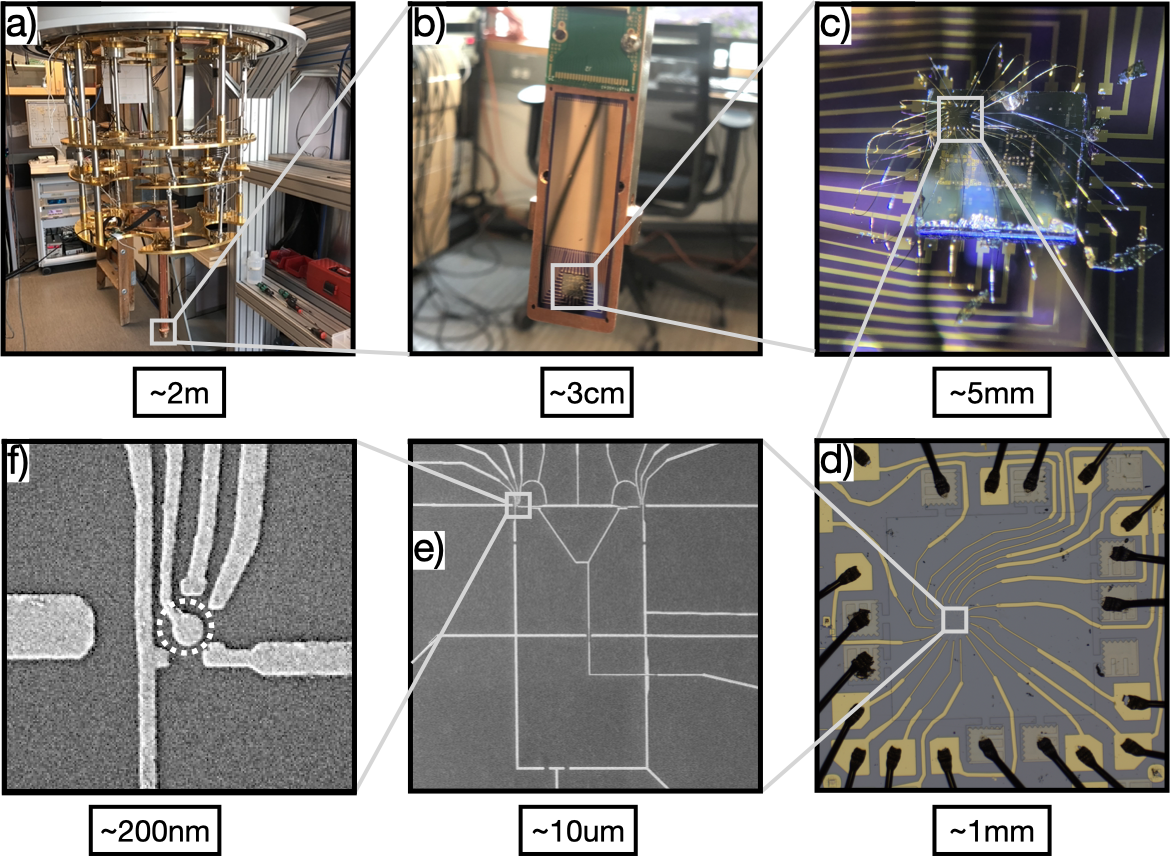
\includegraphics[width=1.0\textwidth]{figures/ch1/crop_FiguresMaster.001.png}
  \caption[Dilution fridge to quantum dot scale breakdown]{\label{fig:ch1/scale_breakdown} 
  % For some options that work with pdf\LaTeX, please see this discussion:
  %  \url{http://tex.stackexchange.com/questions/11839}. 
  Showing the various scales to connect how macro changes affect the nano. (\textbf{a}) A photograph of the Au plated cold plates in our dilution refrigerator. The lowest plate is called the mixing chamber and can reach \qty{7}{mK}. (\textbf{b}) A photograph of the Si chip carrier, onto which the heterostructure is stuck to. (\textbf{c}) An optical microscope image of the heterostructure stuck to the chip carrier. The thin wires are Al wire bonds which connect the device fabricated on the heterostructure to the fridge wires. (\textbf{d}) An optical microscope image of a single mesa on the heterostructure. A mesa is an isolated area of the heterostructure where we fabricate new designs. The black lines around the outside are the wire bonds and the bright Au are the thick (\qty{100}{nm}) `outer gates' which connect to the thin (\qty{10}{nm}) `inner gates'. (\textbf{d}) A scanning electron micrograph (SEM) of the inner gates. The mean free path of the electrons is of order \qty{3}{\mu m}. (\textbf{d}) An SEM image zoom in on the quantum dot. By carefully tuning the voltages on the inner gates, we can create an isolated puddle of electrons, typically with total occupation 0 - 10. 
   }
 \end{center}
\end{figure}


The Kondo effect first discovered in impure bulk metals in the 1930’s~\cite{de_haas} and explained later in the 1960’s~\cite{jun_kondo} has seen significant interest in the field of quantum devices. The high degree of tunability and control in these devices allows for testing predictions of the Anderson model~\cite{costi_kondo_mv_eo_regime}. In quantum devices, a Kondo state is engineered by strongly coupling a quantum dot with an overall spin (odd number of electrons) to two reservoirs. 

% Previous studies measure the conductance through the quantum dot and observe a zero bias peak in the middle of the Coulomb blockade valley. This effect requires strong coupling between the quantum dot and reservoirs.

% In this work, we reduce the coupling so the Kondo effect only enhances the conductance on the shoulder of the conductance peak. By simultaneously measuring the occupation of the quantum dot we can reliably show the small enhancement of conductance due to the Kondo effect. Measuring conductance and occupation at a range of temperatures allows for the determination of relevant parameters for comparison to Numerical Renormalisation Group (NRG) theory calculations. Good agreement is found at a range of coupling strengths. However, a discrepancy is found when the tunnel barriers to the quantum dot are tuned to be asymmetric. The strong asymmetric coupling approaches a regime where the quantum dot is coupled to a single lead. A regime where a recent measurement of the entropy of the Kondo effect found a discrepancy between data and NRG. Interestingly in our experiment, conductance data showed greater Kondo enhancement than NRG, whilst the previously measured entropy showed less Kondo enhancement than NRG. A direct comparison of conductance and entropy measured in the same device with similar settings is required to provide further enlightenment on this discrepancy. 


\chapter{Device Background}\label{cha:device_background}

Before describing measurements at the focus of this thesis, it is important to first introduce the devices we use to engineer interesting states, and the tools we use to measure them. As an overview, we use a material called GaAs/AlGaAs heterostructure, the precise layering of the semiconductors form a two-dimensional electron gas (2DEG) below the surface of the heterostructure. Voltages applied to patterened metallic gates ontop of the heterostructre can control the electrons in the 2DEG allowing for the formation of quantum point contacts (QPCs) and quantum dots  (QDs). Ohmics are used to contact the 2DEG, allowing for transport measurements through such structures. 

\section{Two-Dimensional Electron Gas (2DEG)}



\begin{figure}[!htb]
  \begin{center}
%% psfrag: comment the following line if not using the psfrag package
    % \psfrag{pie makes me happy!}{$\pi$ makes me happy!}
%% includegraphics: comment the following if not using the graphicx package
    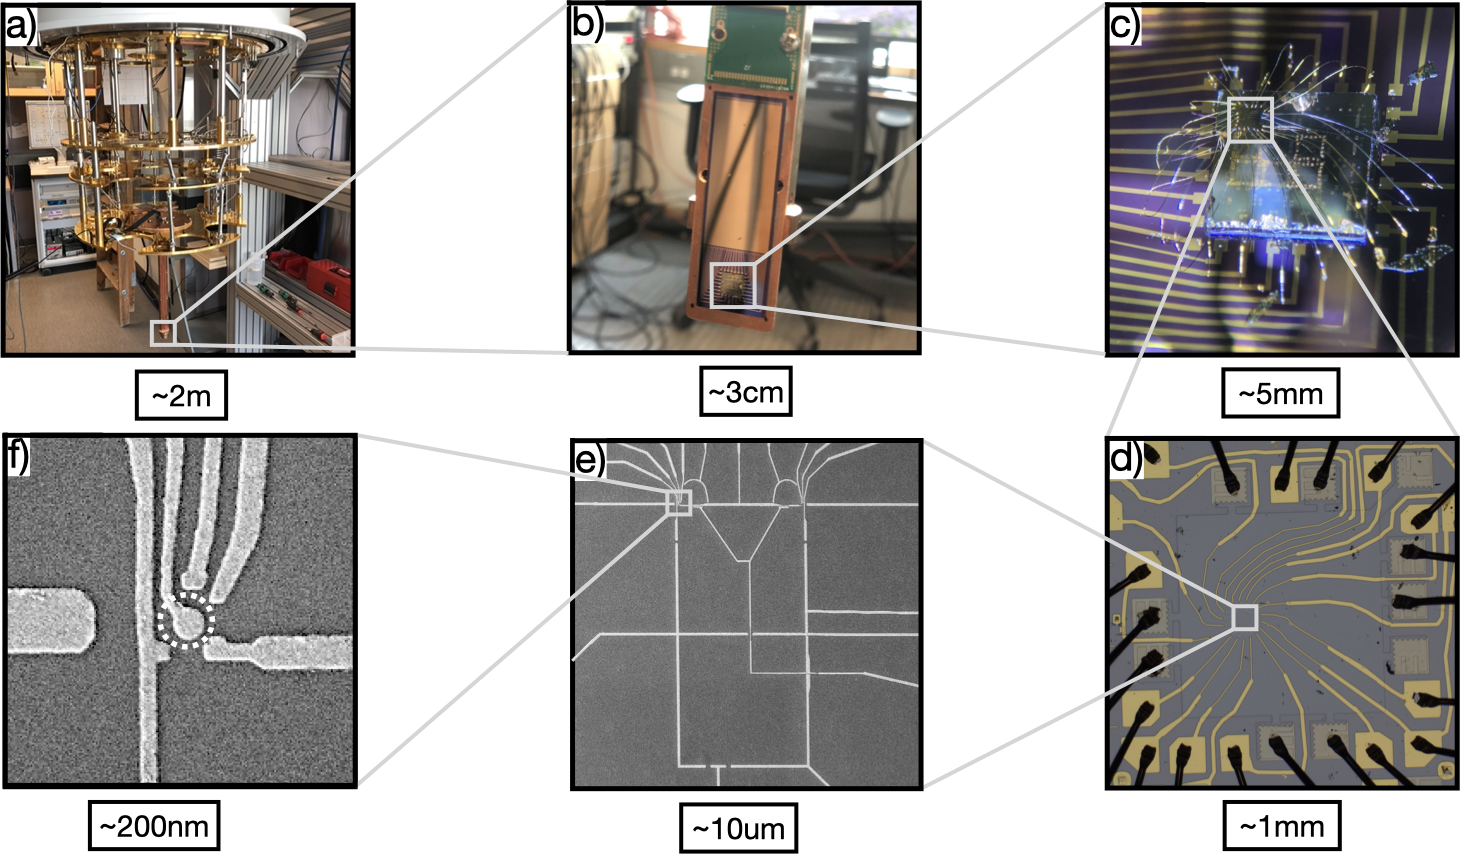
\includegraphics[width=1.0\textwidth]{figures/ch1/crop_PosterFiguresMaster.001.png}
    \caption[Two-dimensional electron gas in a GaAs/AlGaAs heterostructure]{\label{fig:ch1/2deg} 
    % For some options that work with pdf\LaTeX, please see this discussion:
    %   \url{http://tex.stackexchange.com/questions/11839}.  
    CAPTION TO BE ADDED. FIGURE TO BE CHANGED TOI HETEROSTRUCTURE.  
      }
  \end{center}
\end{figure}



The quantum point contacts (QPCs) and quantum dots (QDs) described later in this thesis are engineered in a two-dimensional electron gas (2DEG). A 2DEG can be thought of as a two dimensional plane of electrons which can move freely along the x and y direction, but are tightly confined in the z direction. The 2DEGs' in this thesis are realised in GaAs/AlGaAs heterostructures. A semiconductor heterostructure refers to a material system composed of two or more semiconductor materials with different bandgaps or lattice constants that are layered together Fig.~\ref{fig:ch1/2deg}. These layers are typically grown on top of each other using techniques such as molecular beam epitaxy (MBE). The heterostructures in this thesis are grown by Michael Manfra's lab at Purdue University [reference XXX]. 

There are two characteristics of this heterostructure which give rise to a 2DEG. Firstly, $\mathrm{Al_xGa_{1-x}As}$ has a tunable bandgap ranging from 1.42 - \qty{2.16}{eV} [REFERENCE XXX] whilst GaAs has a bandgap of \qty{1.42}{eV}. Secondly, an n-type dopant layer is sandwiched between the $\mathrm{Al_xGa_{1-x}As}$ layers. The smaller bandgap of GaAs allows the electrons from the donar atoms in the dopant layer to drop into the GaAs conduction band resulting in a triangular potential well. This triangular well contains of multiple sub-bands. The second sub-band is $\qty{\sim 150}{meV}$ above the first and will remain unoccupied as than energy gap is much greater than measurement temperatures $\qty{500}{mK}\sim\qty{43}{\mu eV}$ and source-drain bias $\qty{100}{\mu eV}$, hence, the electron gas can be considered two-dimensional.

Efforts are made to keep the heterostructure and 2DEG clean and defect free. A \qty{7}{nm} cap of GaAs is placed ontop of the heterostructure to prevent oxidation. A small lattice mis-match between the GaAs and AlGaAs layers keeps the number of boundary defects in the 2DEG plane low. The \qty{30}{nm} AlGaAs buffer layer between the 2DEG and dopants helps prevent defects near the 2DEG plane. The resulting 2DEGs' has a high mobility $\mathrm{\mu_e}~=~\qty{2.56e6}{cm^2/Vs}$ and electron density $\mathrm{n}~=~\qty{2.42e11}{cm^{-2}}$

Fabrication details on these devices `re described in Appendix [XXX]. As an overview, the heterostructure is divided into separate areas with isolated 2DEGs' by etching away the top layers of the heterostructure to remove the 2DEG. Contact to the 2DEG is made with ohmics contacts. These are made by annealing a layer of Ni-Au-Ge, the metal diffuses through the heterostructure and forms an electrical connection to the 2DEG. An insulating dielectric of \qty{10}{nm} $\mathrm{Al_2O_3}$ is deposited across the surface of the heterostructure to limit leakage from the metallic gates.  A thin layer (\qty{10}{nm}) of Au is deposited to form the inner gates which we design to form the QPCs and QDs. In a second step, a thick layer (\qty{100}{nm}) of Au is deposited (our outer gates) to connect the inner gates to square bond pads. Wire bonds are then made from chip carrier to the square bond pads which allows for connection between fridge wiring and the quantum device. 




\afterpage{\clearpage}
\section{Quantum Point Contact (QPC)}

\begin{figure}[!htb]
  \begin{center}
%% includegraphics: comment the following if not using the graphicx package
    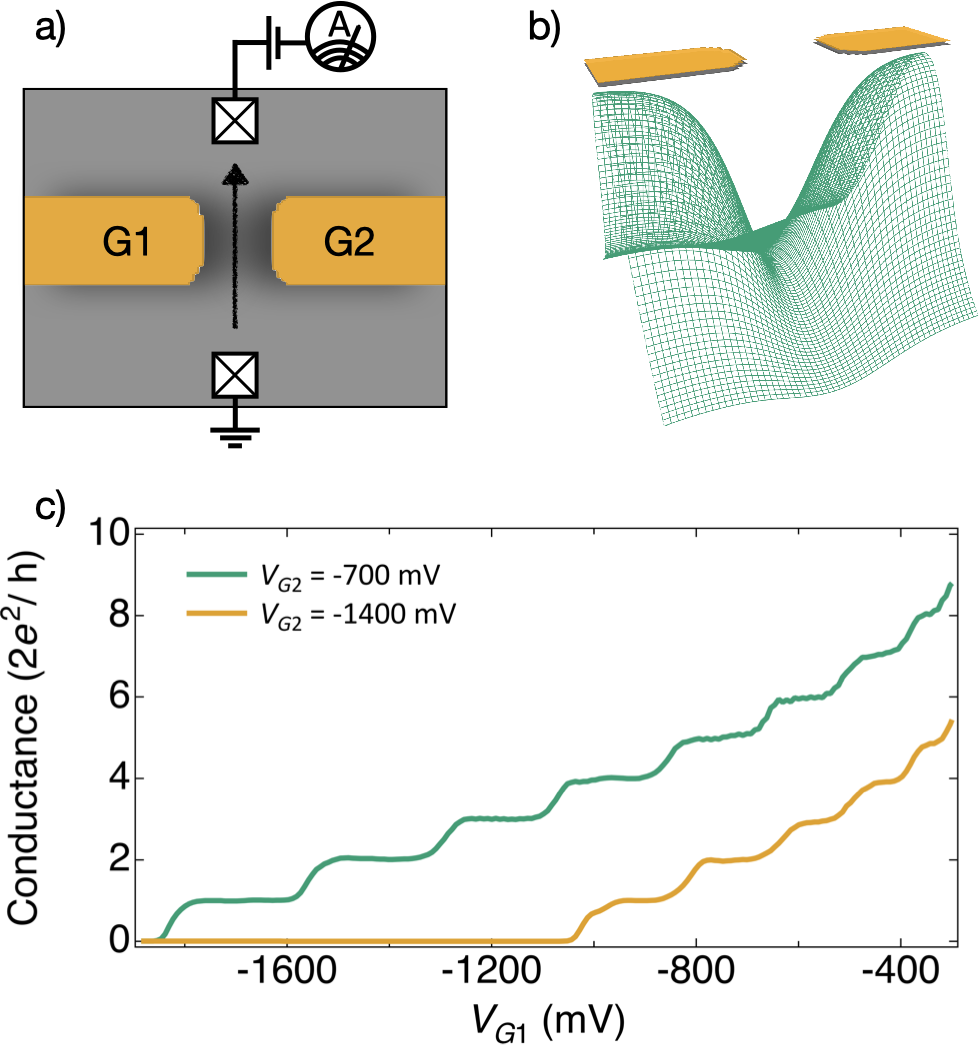
\includegraphics[width=0.9\textwidth]{figures/ch1/crop_PosterFiguresMaster.002.png}
    \caption[Conductance through a quantum point contact]{\label{fig:ch1/qpc_intro} 
    % For some options that work with pdf\LaTeX, please see this discussion:
    %   \url{http://tex.stackexchange.com/questions/11839}.  
    (\textbf{a}) A graphic representation from a top-down view of a quantum point contact (QPC). The gold fingers are the metallic gates where negative voltages can be applied to. The grey is where the electrons in the 2DEG can go dependant on the amount of negative voltage applied to the gates. The crossed squares are ohmic contacts to the 2DEG so that bias can be applied and the conductance through the QPC is measured. (\textbf{b}) is a representation of the electric potential the electrons see in the 2DEG due to negative voltage applied to the gates. With sufficient negative voltages applied to the gates, the electrons cannot overcome the potential barrier under the gate and flow through the middle. (\textbf{c}) is a measurement showing the quantised conductance through a QPC as the voltage on G1 becomes more negative. The voltage on the gates can be made negative enough so that electrons cannot tunnel across the potential barrier and hence we measure 0 conductance. 
      }
  \end{center}
\end{figure}

In this thesis a quantum point contact (QPC) is one-dimensional channel connected to a source and drain reservoir Fig.~\ref{fig:ch1/qpc_intro}. A one-dimensional channel in the 2DEG is engineered by putting sufficient negative voltage on metal gates deposited on the surface of the heterostructure. By applying a potential bias between the ohmics a current will flow. The more negative the voltage on the gate, the higher the potential barrier is for the electrons in the 2DEG. A large enough potential barrier can stop the electrons flowing underneath the gate (called 'depletion'), however, they can still flow between the gates. It normally requires a more negative voltage to stop electrons flowing between the gates (called 'pinch-off'). A QPC length is the length of the one-dimensional channel and the width is the empty space between gates. In our devices, QPCs' have lengths 50~-~\qty{350}{nm} and widths 100~-~\qty{350}{nm}.

If the width of the QPC is comparable to the Fermi wavelength, the electrons will be quantised in the x-direction and free to move in the y-direction. The confining potential in the x-direction can be modelled as a parabolic potential and hence the allowed 1d sub-bands will resemble solutions to the harmonic oscillator Fig.~\ref{fig:ch1/qpc_intro}\textbf{b}. In the absence of a magnetic field, each occupied sub-band contributes $\mathrm{2e^2/h}$ to the conductance. The $2$ comes from the spin degeneracy of the electrons which can be lifted with magnetic field. When measuring the conductance through a QPC as it is pinched off Fig.~\ref{fig:ch1/qpc_intro}\textbf{c} we see the quantised conductance as plateaus at integer values of $\mathrm{2e^2/h}$. At zero temperature the conductance would increase in sharp steps but this is smeared out by temperature in a real measurement.

In our devices, QPCs are used to form tunable tunnel barriers between a quantum dot and a reservoir (described in the next section) and charge sensors which are used to measure the charge around a quantum dot. 




\afterpage{\clearpage}
\section{Quantum Dot (QD)}

In this thesis a quantum dot (QD) is zero-dimensional structure, it can be formed by connecting a potential well to source and drain reservoirs through tunnel barriers. The tunnel barriers are formed by QPCs. Similar to a QPC, the potential well is formed by applying negative voltages to gates to confine a small region in the 2DEG Fig.~\ref{fig:ch1/dot_intro}\textbf{a}. The first characteristic of these dots is the charging energy $\mathrm{E_C}$, this is the energy required to add or remove an electron from the quantum dot due to the Coulomb force. Under certain conditions the charge in the quantum dot is quantised and equal to $\mathrm{Ne}$, where $\mathrm{N}$ is the total number of electrons and $\mathrm{e}$ is the charge of a single electron. The two conditions are $\mathrm{R_t}>>\mathrm{h/e^2}$ and $\mathrm{E_C}>>\mathrm{k_BT}$. The first condition is the resistance of the tunnel barriers $\mathrm{R_t}$, should be greater than the resistance quantum $\mathrm{h/e^2}=\qty{25.813}{k\Omega}$. Qualitatively we can think of the barriers being large enough so the electron is located either in the source or drain leads, or in the quantum dot. The second condition is the charging energy should be larger than the thermal energy of the system. These conditions lead to quantised charge in the quantum dot, but quantised charge can be seen in small metallic islands. The second characteristic scale of a quantum dot is if the size is comparable to the deBroglie wavelength (XXX). A 1d box of size $\mathrm{L}$ has energy level spacing $\mathrm{\Delta E}=(\mathrm{N}/4)\hbar^2\pi^2 / \mathrm{m^*L^2}$, where $\mathrm{m^*}=0.67\mathrm{m_e}$ is the effective mass of electrons. Similar to seeing the quantisation of charge in the quantum dot, to see the energy level spacing the condition should be satisfied $\mathrm{\Delta E}>>\mathrm{k_BT}$ where the energy level spacing is greater than the thermal energy of the system. 

\afterpage{\clearpage}
\subsection{Conductance Through a Quantum Dot}

\begin{figure}[!htb]
  \begin{center}
%% includegraphics: comment the following if not using the graphicx package
    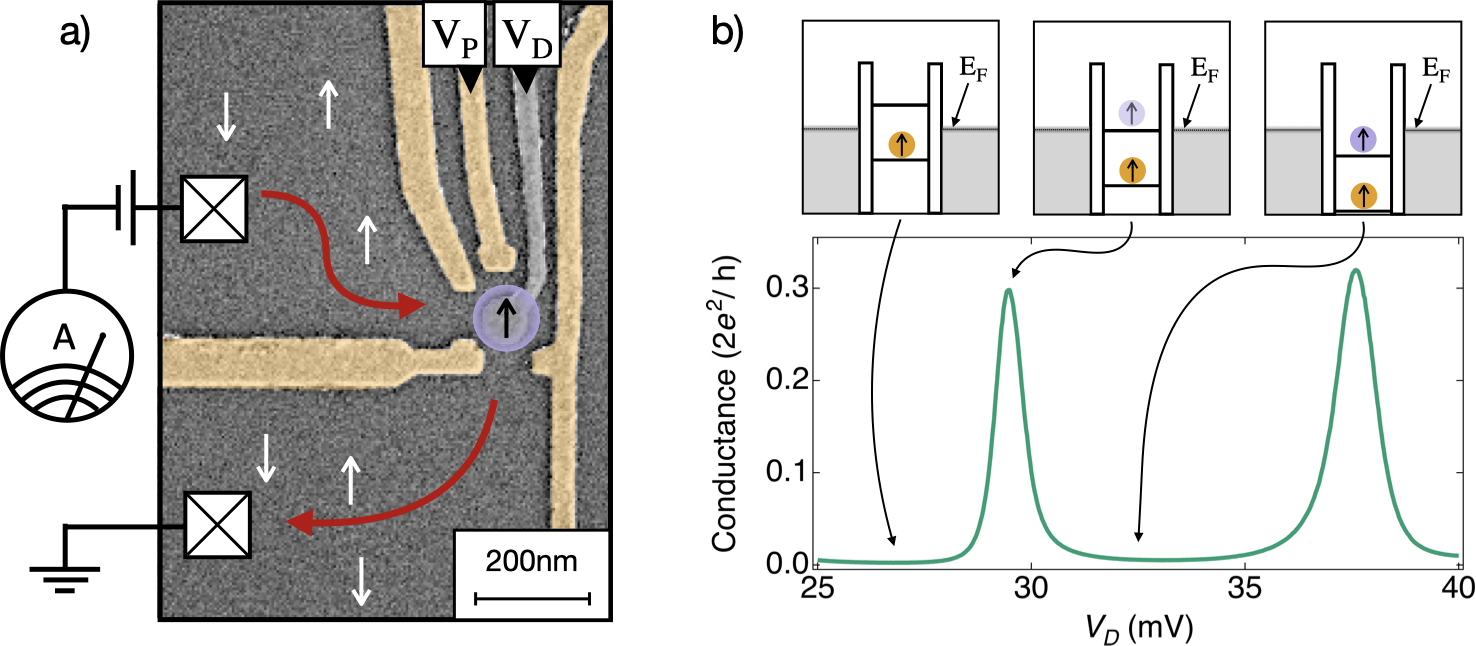
\includegraphics[width=1.0\textwidth]{figures/ch1/crop_PosterFiguresMaster.003.png}
    \caption[Conductance through a quantum dot]{\label{fig:ch1/dot_intro} 
    % For some options that work with pdf\LaTeX, please see this discussion:
    %   \url{http://tex.stackexchange.com/questions/11839}.  
    (\textbf{a}) an SEM image of the gates used to define a quantum dot. The gold coloured gates indicate sufficient negative potential is applied so that the 2DEG below is depleted. The gates V\textsubscript{P} or V\textsubscript{D} have the biggest effect on dot energy without changing other energies. The crossed are ohmic contacts which contact the 2DEG. By applying a small bias we measure the conductance through the quantum dot. (\textbf{b}) are Coulomb blockade energy diagrams illustrating how the conductance varies as an electron enters the quantum dot. The grey boxes represent the continuous energy level of electrons in the leads. The white rectangles represent tunnel barriers into and out-of the quantum dot. The rate of tunneling is described by the parameter $\Gamma$, the wider (narrower) the barrier, the smaller (larger) the rate of tunneling. (\textbf{c}) is a measurement showing the conductance through a quantum dot as a single electron (in purple) is added. From left to right: Electrons in the leads cannot tunnel into the quantum dot as there is no available energy level and hence we measure zero conductance. As V\textsubscript{D} is made less negative, the dot energy lowers and electrons can tunnel into the dot and back out. We measure a maximum in conductance when the dot energy is aligned with the leads. Once the dot energy falls below the level of the leads there is again no available energy level and the dot is insulating. 
      }
  \end{center}
\end{figure}

A quantum dot is formed by applying negative voltages to confine a small region in the 2DEG Fig.~\ref{fig:ch1/dot_intro}\textbf{a}.
Each of the gates near the quantum dot are capacitively coupled to the different parameters that determine the different energies in the dot. However, the gates geometry was designed for certain gates to affect some energies more than others. In Fig.~\ref{fig:ch1/dot_intro}\textbf{a}, $\mathrm{V_{LC}}$ is the 'left-coupling' gate and the strongest effect on the left tunnel barrier along with $\mathrm{V_{N}}$. $\mathrm{V_{N}}$ is the 'nose' gate and effects both coupling equally, it also has a large effect on the dot energy and can push the location of the electron wave function closer to $\mathrm{V_{CSS}}$. $\mathrm{V_{CSS}}$ is the 'charge sensor spine' the charge sensor is discussed in the next section but it is important for the wavefunction of the electron to be close to $\mathrm{V_{CSS}}$ for higher sensitivity of the charge sensor. $\mathrm{V_{P}}$ is the 'plunger' and is used primarily to control the dot energy as it is far from the tunnel barriers. By making this gate less negative the dot energy decreases and at some point another electron can enter the dot. $\mathrm{V_{D}}$ is the 'dot' gate, this gate is operated different to the other gates as it lies right above where the dot lives. This gate is most strongly coupled to the dot energy and we use this gate to add or remove single electrons into the quantum with fine control. This gate is normally at positive voltage values to help form the potential well as negative voltages will form a donut shaped potential. 



\afterpage{\clearpage}
\subsection{Charge Sensing a Quantum Dot}

\begin{figure}[!htb]
  \begin{center}
%% includegraphics: comment the following if not using the graphicx package
    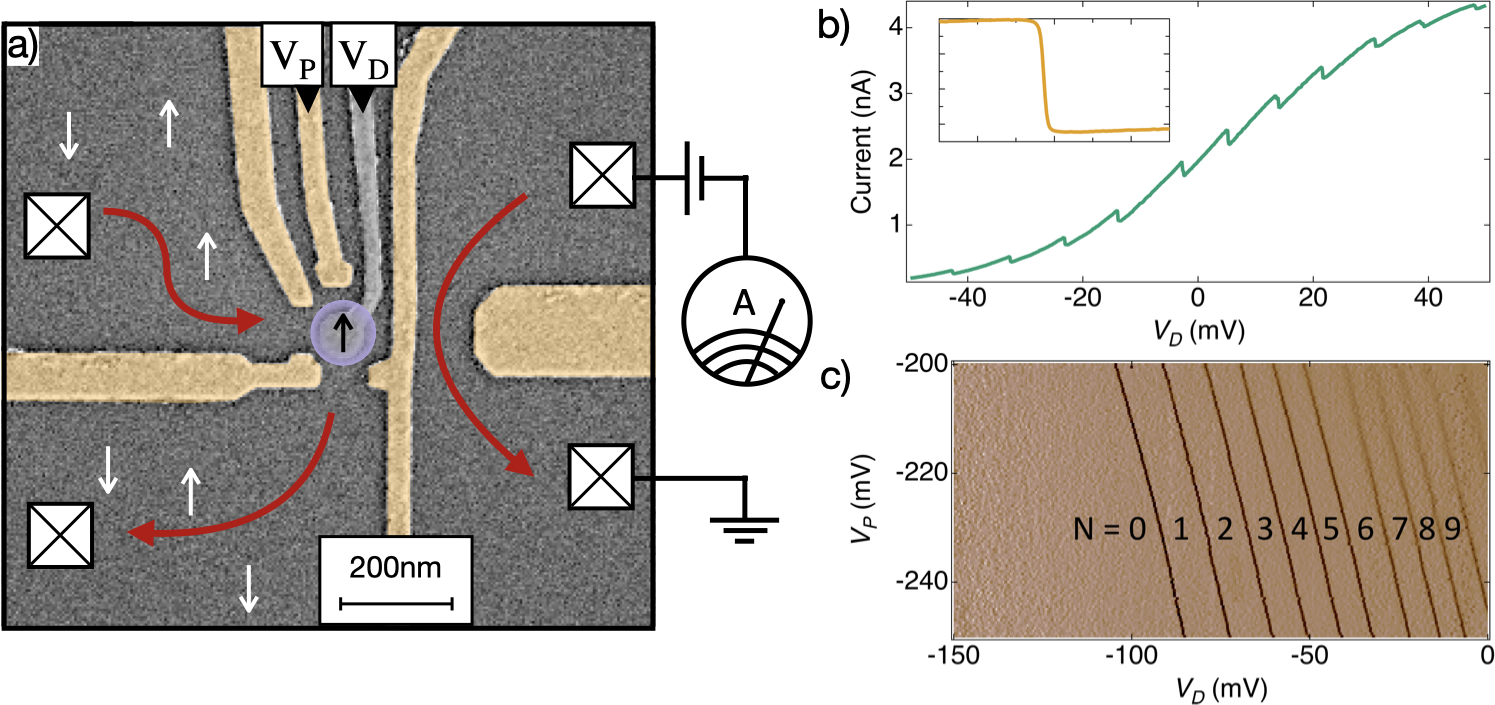
\includegraphics[width=1.0\textwidth]{figures/ch1/crop_PosterFiguresMaster.004.png}
    \caption[Charge sensing a quantum dot]{\label{fig:ch1/ct_intro} 
    % For some options that work with pdf\LaTeX, please see this discussion:
    %   \url{http://tex.stackexchange.com/questions/11839}.  
    (\textbf{a}) An SEM image of the gates used to define a quantum dot. The gold coloured gates indicate sufficient negative potential is applied so that the 2DEG below is depleted. The gates V\textsubscript{P} or V\textsubscript{D} have the biggest effect on dot energy without changing other energies. The crossed are ohmic contacts which contact the 2DEG. V\textsubscript{CSQ} is used to form a QPC near the quantum dot. By setting up the QPC on a steep slope the current through the QPC is sensitive to nearby changes in charge. (\textbf{b}) measuring the current across the charge sensing QPC. As V\textsubscript{D} becomes less negative the current through the QPC increases. The downward jumps in current are a result of the negative repulsion from electrons entering the quantum dot. The subfigure (yellow) shows a zoomed in scan over one of these transitions. (\textbf{c}) A 2d map showing how the occupation of the quantum dot changes as a function of V\textsubscript{P} and V\textsubscript{D}. The data is the differentiated current through the charge sensor. The differentiated steep slopes of the charge transitions show up as sharp peak which is useful for locating charge transitions when there is a large change in background current. 
      }
  \end{center}
\end{figure}

A charge sensor is a way to measure the charge around the quantum dot and if correctly tuned it is very sensitive to the additional charge of an electron that enters a quantum dot. It is formed by adding a QPC in close proximity to the quantum dot Fig.~\ref{fig:ch1/dot_intro}\textbf{a}. A QPC can be tuned to have a steep slope or plateau  Fig.~\ref{fig:ch1/qpc_intro}\textbf{c}. When used as a charge sensor, the QPC is tuned to be on a steep slope. This is useful as small changes in nearby potentials (x-axis of a QPC trace) show up as large changes in the current measured through the QPC. In Fig.~\ref{fig:ch1/dot_intro}\textbf{b} the QPC is set up on a steep slope and V\textsubscript{D} is swept from negative to positive to lower the dot energy so that electrons can hop in. The background increase in current is due to the capacitive coupling of V\textsubscript{D} as it is swept to more positive values. But once an electron can hop into the quantum dot the extra negative charge shows up as a small but sharp decrease in current which we call a 'charge transition'. The derivative of the current is useful for quickly identifying electrons entering the quantum dot as the steep slope of the charge transition shows up as a large negative spike. One of the functions of the charge sensor is to count how many electrons are in the quantum dot Fig.~\ref{fig:ch1/dot_intro}\textbf{c}. By making V\textsubscript{D} more negative whilst keeping the tunnel barrier open for electrons to enter the quantum dot we will at some point stop seeing charge transitions signalling the last electron. Also, a 2d sweep with a different gates on either axis tells us the relative cross capacitance between each gate on the dot energy. From Fig.~\ref{fig:ch1/dot_intro}\textbf{c}, a \qty{-50}{mV} change on V\textsubscript{D} remove $\sim~4$ electrons but \qty{-50}{mV} change on V\textsubscript{P} only removes $\sim~2$ electrons.



\afterpage{\clearpage}
\section{Electron Temperature from Charge Transitions}

\begin{figure}[!htb]
  \begin{center}
%% includegraphics: comment the following if not using the graphicx package
    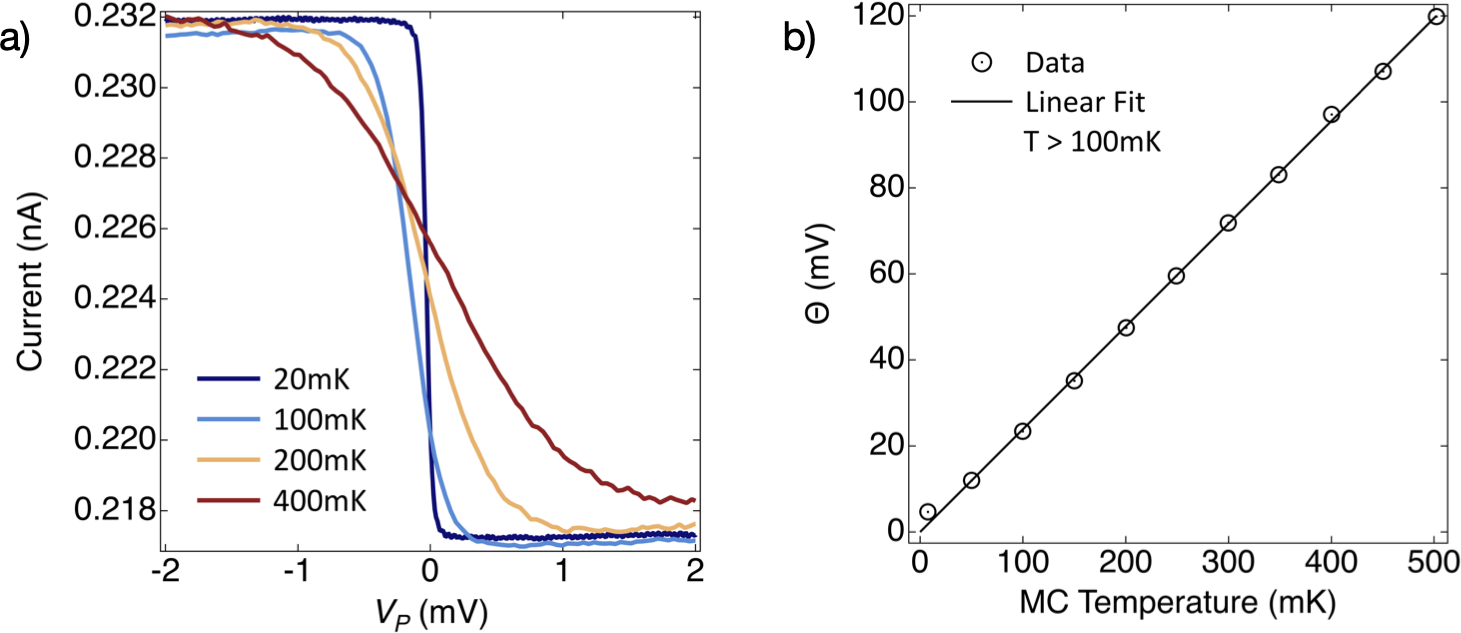
\includegraphics[width=1.0\textwidth]{figures/ch1/crop_PosterFiguresMaster.005.png}
    \caption[Calculating the electron temperature]{\label{fig:ch1/electron_temp} 
    % For some options that work with pdf\LaTeX, please see this discussion:
    %   \url{http://tex.stackexchange.com/questions/11839}.  
    (\textbf{a}) A weakly coupled charge transition measured at different fridge temperatures. The broadening of a weakly coupled charge transition is linearly proportional to its temperature. (\textbf{b}) A plot of the calculated broadening ($\Theta$) of the charge transition at different fridge temperatures. At fridge temperatures \qty{>100}{mK}, the increase in the charge transition broadening is linear. This indicates the electrons are well thermalised to the fridge. A linear fit to fridge temperatures \qty{>100}{mK} is extrapolated to base temperature to calculate the temperature of the electrons given the measure broadening. 
      }
  \end{center}
\end{figure}

Measuring charge transitions with the charge sensor lets us count the number of electrons in the quantum dot or the relative cross capacitance between different gates on the dot energy. But it can also be used to measure the temperature of the electrons in the 2DEG. When the broadening of a charge transition is due to the thermal energy of the system rather than the coupling strength to the source and drain leads ($\Gamma/\mathrm{T} << \mathrm{k_B T}$), the charge transition is described as being temperature broadened. The current through the charge sensor for a temperature broadened (weakly coupled) charge transition has lineshape,

\begin{equation}\label{eq:cs_lineshape}
  \mathrm{I_{CS}} = 
  \mathrm{I_{amp}}
  \tanh
  \left( 
  \frac{\mathrm{V_P - V_{mid}}}{2\Theta}
  \right) + 
  \gamma \mathrm{V_P}
  + \mathrm{I_{const}}
\end{equation}

where $\mathrm{I_{CS}}$ is the current through the charge sensor. $\mathrm{I_{amp}}$ is the amplitude of the charge transition, $\mathrm{V_{P}}$ is the voltage on the sweep gate to sweep over the charge transition, $\mathrm{V_{mid}}$ is the mid point of the charge transition. $\Theta=\frac{\mathrm{k_B}T}{\mathrm{\alpha e}}$ is the thermal broadening in units of gate voltage, where $\alpha \equiv \frac{\mathrm{d\epsilon}}{\mathrm{dV_P}}$ is a leverarm that relates changes in a gate voltage to changes in the dot energy. $\gamma$ is the cross capacitance between the sweep gate and the current through the charge sensor. $\mathrm{I_{const}}$ is a constant current offset.

The broadening of a temperature broadened charge transition can be used to determine the temperature of the electrons in thee 2DEG as the broadening is linearly proportional to the temperature ($\Theta\propto\mathrm{T}$) of the electrons Fig.~\ref{fig:ch1/electron_temp}\textbf{a}. At high fridge temperatures, the electrons in the 2DEG are in thermal equilibrium with the fridge. But as the fridge reaches base temperature (\qty{7}{mK}), the electrons in the 2DEG will not be in equilibrium due to poor thermal contact and source drain biases that can heat the electrons (i.e. \qty{1}{\mu eV}~=~\qty{11.6}{mK}). 
% Also charge noise that shifts the charge transition left or right in gate space 
To determine the proportionality constant between the broadening and temperature, charge transitions are measured at a range of fridge temperatures from \qty{8}{}~-~\qty{500}{mK}. Each charge transition will be measured quickly ($\sim$\qty{0.5}{s}) and repeated many times ($\sim300$). Any traces with large jumps in current near the charge transition ('charge jumps') are thrown out, and the remaining traces are then centered and averaged. The quick scans and averaging reduces additional broadening that come from charge motion in the dopant layer which shifts the charge transition left and right. The amount charge motion in the dopant layer scales between $\mathrm{1/f}$ and $\mathrm{1/f^2}$ [XXX]. Each charge transition is then fit using Eq.~\ref{eq:cs_lineshape} and the calculated $\Theta$ is plotted versus the fridge temperature Fig.~\ref{fig:ch1/electron_temp}\textbf{b}. A linear fit to $\Theta$ between \qty{100}{}~-~\qty{500}{mK} determines the proportionality constant. This is then used to convert the $\Theta$ measured as base temperature into the effective temperature of the electrons in the 2DEG. In this fridge we determine a base electron temperature of \qty{20}{mK}.


\subsection{Charge Sensing with a Virtual Gate}

\begin{figure}[!htb]
  \begin{center}
%% includegraphics: comment the following if not using the graphicx package
    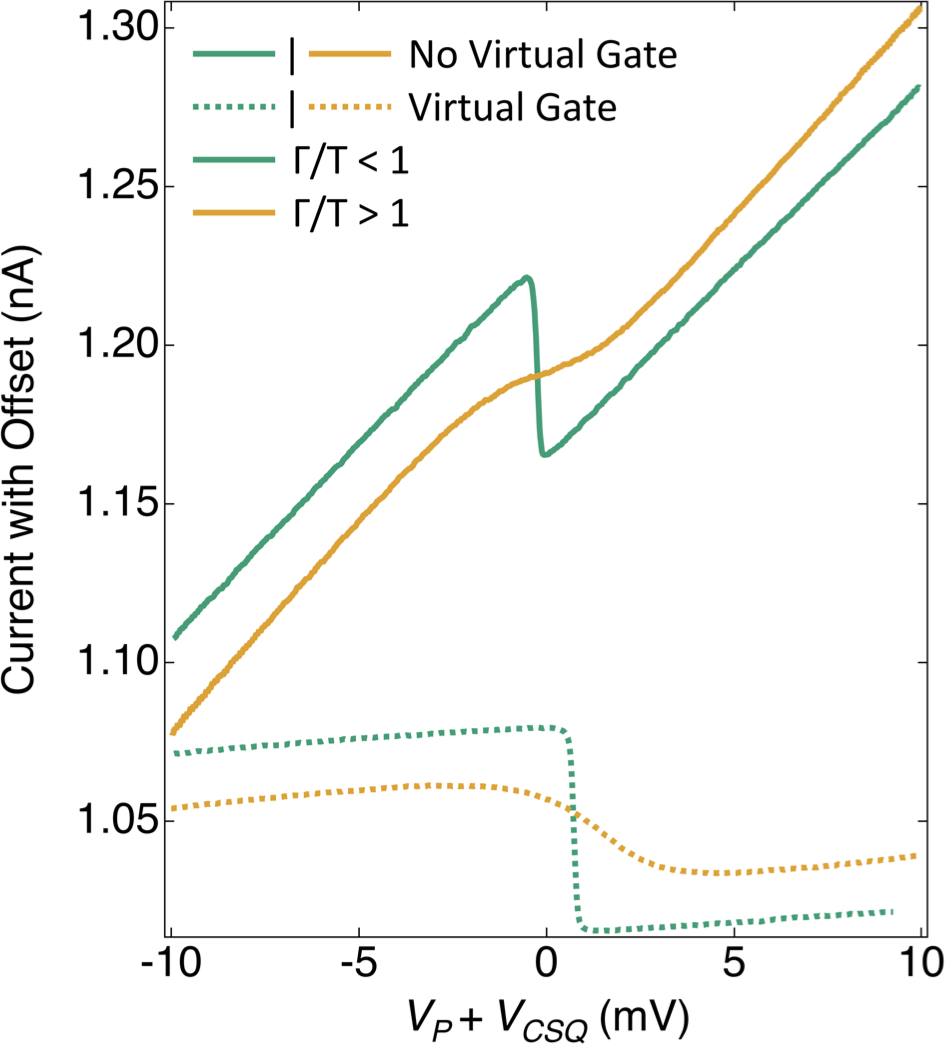
\includegraphics[width=0.8\textwidth]{figures/ch3/crop_PosterFiguresMaster.009.png}
    \caption[Measuring charge transitions with and without a virtual gate]{\label{fig:ch3/virtual_gate_example} 
    % For some options that work with pdf\LaTeX, please see this discussion:
    %   \url{http://tex.stackexchange.com/questions/11839}.  
    Data of a weakly (green) and strongly (yellow) coupled charge transition scanned with a single gate V\textsubscript{P} (solid line) and a virtual gate  V\textsubscript{P}~+~V\textsubscript{CSQ} (dashed line). The traces have been offset in current for ease of comparison. V\textsubscript{P} has a large effect on the dot energy, however, it also changes other parameters due to capacitive coupling. Here, a virtual gate is used to change the dot energy whilst keeping the current through the charge sensor constant. This helps with visually identifying strongly coupled charge transitions which become very broadened. More importantly, the charge sensor stays in the linear regime where changes in the potential are linearly proportional to changes in the current. Note the x-axis is only showing the value of V\textsubscript{P}. As V\textsubscript{P} is swept negative to positive, V\textsubscript{CSQ} is swept positive to negative.}
  \end{center}
\end{figure}


Temperature broadened transitions are straightforward to fit as they are described by an analytic function where the broadening is due to a single parameters and the sharpness of the transitions makes visual inspection of the fits trivial. The work in this thesis focuses on coupling strengths of $\Gamma/\mathrm{T}>1$. The charge transition at these larger coupling strengths becomes very spread out and it can be tricky to visually inspect the quality of the fits. 

One way to tackle this problem is by using a virtual gate. In general, a virtual gate is a name give to a combination of gates that when varied, change a parameter of the dot whilst keeping other parameters constant. The main parameters we think about are the dot energy $\mathrm{\epsilon}$, left coupling $\mathrm{\Gamma_L}$, right coupling $\mathrm{\Gamma_R}$ and current through the charge sensor $\mathrm{I_{CS}}$. An example usage would be a virtual gate that controls the left coupling $\mathrm{\Gamma_L}$ only. A combination of V\textsubscript{LC} and V\textsubscript{P} would be used. V\textsubscript{LC} to primarily changed the left coupling $\mathrm{\Gamma_L}$ and V\textsubscript{P} to offset any changes to the dot energy. 

In the context of this thesis, only a virtual gate that changes the dot energy but keeps the current constant through the charge sensor is used. Fig.~\ref{fig:ch3/virtual_gate_example} shows the effect of this virtual gate on a weakly coupled ($\Gamma/\mathrm{T}<1$) and strongly coupled ($\Gamma/\mathrm{T}>1$) charge transition. By sweeping V\textsubscript{CSQ} in the opposite direction of V\textsubscript{P}, the cross-capacitive effect of V\textsubscript{P} on the charge sensor is largely removed. 


\afterpage{\clearpage}
\section{Measurement Pocedures}

\subsection{Cooldown Bias}
At room temperature, $+$\qty{200}{mV} is applied to all the gates forming the dot and charge sensor (apart from V\textsubscript{D}). This positive bias repels the postive charge underneath the gates in the dopant layer. Once the device reaches \qty{10}{K}, the dopants are frozen in and an effective potential is seen by the electrons in the 2DEG due to the absence of positive charge. Cooling with bias has two advantages. One, it reduces the charge noise [XXX]. Two, it reduces the amount of negative potential required on the gates. The effective potential from the positive bias is roughly equal to a negative bias of equal magnitude when the device is cold (i.e. $+$\qty{200}{mV} cooldown bias $\approx$ $-$\qty{200}{mV}). This is useful as the fine gates can 'blow-up' (in reality the metal gates will lift off a little from the heterostructure surface) from high voltages rendering the device un-measurable. The fine gates are also sensitive to static discharge, so we put \qty{1}{M\Omega} of inline resistance on all of the gates.   

\subsection{Gate Dividers}
When measuring charge transitions with a virtual gate we often require fine gate control at large voltages. For example, V\textsubscript{P} may need a voltage of $-$\qty{500}{mV} but a resolution of \qty{0.001}{mV}. Digital-to-analog converter (DAC) channels are used to apply the voltage on the gates. The DACs have a range of $\pm$\qty{10}{V}, with 16-bit resolution. This puts a lower bound on the step size of \qty{0.305}{mV} ($\mathrm{\qty{20}{V}/2^{16}}$). To achieve achieve the large voltage range with high resolution, two DACs are connected to the same gate. One DAC channel is used to cover a wide voltage range whilst the other is used for fine control by adding a voltage divider in-line. Voltage dividers between $20$ and $100000$ are commonly used to achieve the required resolution (up to \qty{3}{nV}). All of the voltages in this thesis have been converted to the real voltage applied to the gate (i.e. not the voltage output on the DAC). However, we commonly use the fine gate to sweep over transitions and do not show the rough gate voltage that is also applied to the same gate for clarity. 




 





\chapter{Conductance in the Kondo Regime}\label{cha:kondo_conductance}


\epigraph{Ní dhéanfaidh smaoineamh an treabhadh duit.}{Irish proverb}


\section{Introduction}
\noindent This chapter serves as an introduction to the Kondo effect. The history of the Kondo effect began with a measurement that showed a strange behaviour (resistivity minimum with decreasing temperature) in impure gold wires~\cite{de_haas}. It took thirty years before Jun Kondo explained this effect, hence the name `Kondo effect'~\cite{jun_kondo}. After another thirty years, advancements in technology revealed the quantum dot as an exciting platform to explore the Kondo effect due to its high degree of in-situ tunability~\cite{goldhaber_first_kondo}. 



% \afterpage{\clearpage}
\section{Kondo Effect in Bulk Materials}


In the 1930s, it was found that the resistivity would surprisingly increase in impure gold wires at low temperatures~\cite{de_haas}. This was unexpected as due to electron-phonon scattering, the resistivity should decrease with $\mathrm{T^5}$ before saturating at some non-zero resistivity. Data from the original experiment is plotted in Fig.~\ref{fig:ch2/kondo_bulkmetal} with expected electron-phonon dependence. Over the coming years, it was found that metals with magnetic impurities had a similar behaviour~\cite{still_irresistible}.


\begin{figure}[!hbt]
 \begin{center}
%% includegraphics: comment the following if not using the graphicx package
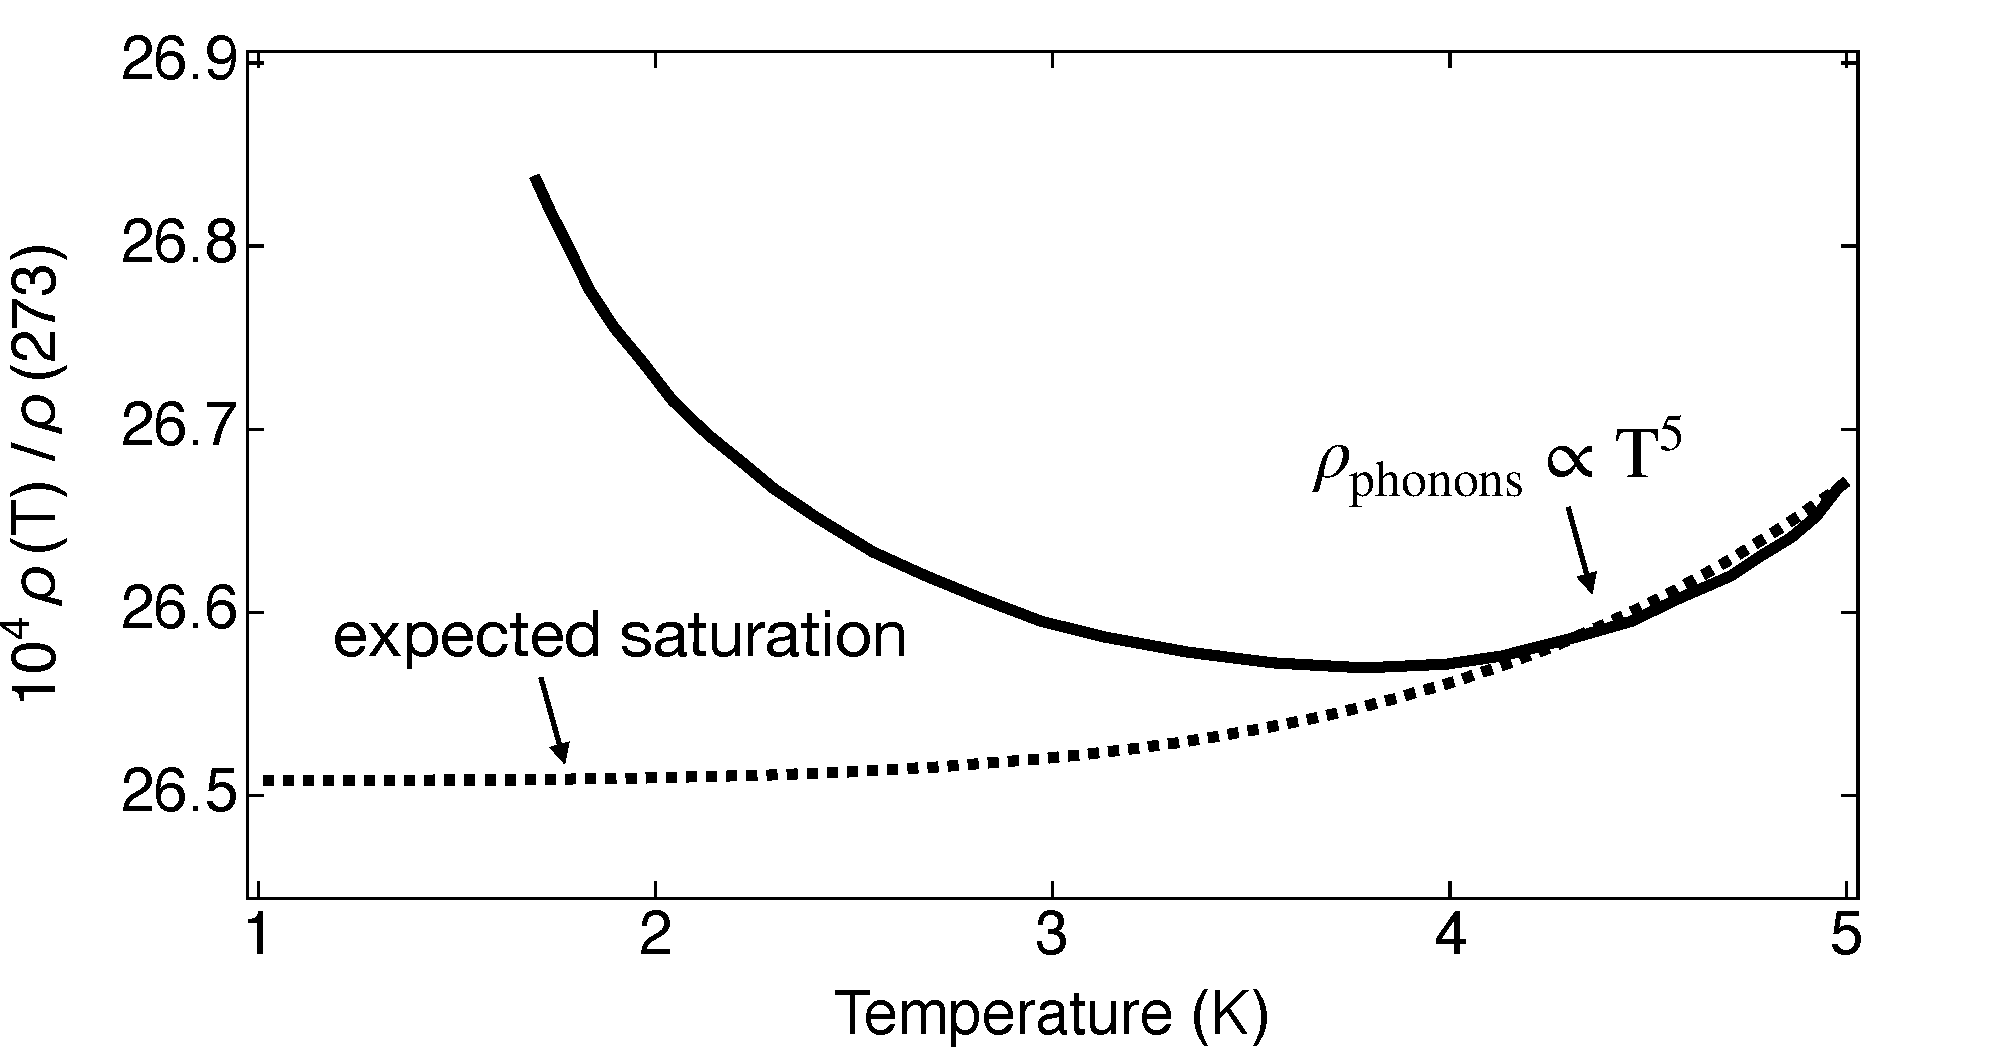
\includegraphics[width=0.9\textwidth]{figures/ch2/figure9.pdf}
\caption[Kondo Effect in Bulk Materials]{\label{fig:ch2/kondo_bulkmetal} 
% For some options that work with pdf\LaTeX, please see this discussion:
%\url{http://tex.stackexchange.com/questions/11839}. 
Temperature dependence of the resistivity, $\mathrm{\rho}$. In simple metals, the resistivity initially decreases as $T^5$ due to electron-phonon scattering. However, due to the Kondo effect, the resistivity reaches a minimum before increasing logarithmically with decreasing temperature. The data used for this figure was obtained from~\cite{de_haas}.
 }
 \end{center}
\end{figure}




It took until 1964 for a theoretical explanation of the resistivity minimum~\cite{jun_kondo}. Jun Kondo used the s-d model, which couples a metal (non-magnetic, s-band) to a magnetic impurity (unfilled d-level). By looking at the second Born approximation, a logarithmic term appeared, which added a large correction to the resistivity at low $\mathrm{T}$. This contribution comes from a process where spin exchange interactions occur. This work showed that a magnetic impurity at low temperatures can give rise to an alternative scattering process, involving a temporary exchange of spin states between the magnetic impurity and surrounding conduction electrons. 

\begin{figure}[!hbt]
 \begin{center}
%% includegraphics: comment the following if not using the graphicx package
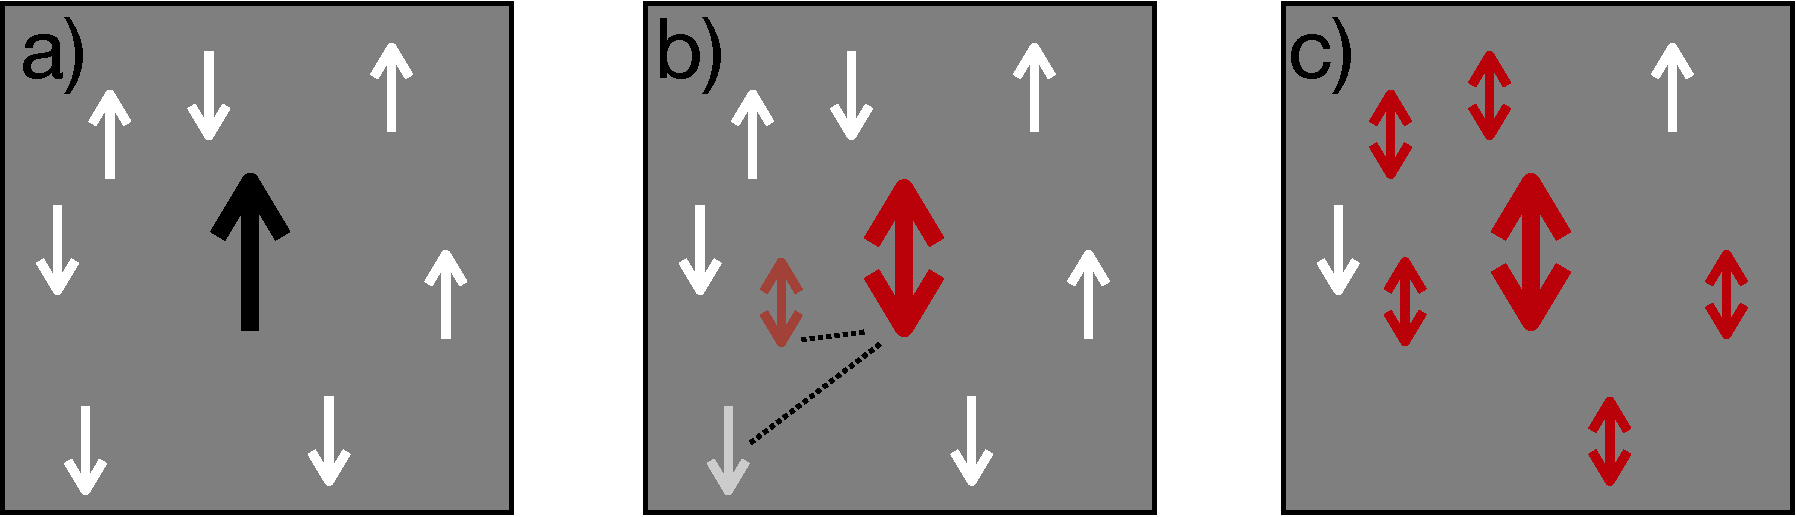
\includegraphics[width=0.9\textwidth]{figures/ch2/figure10.pdf}
\caption[Kondo Effect Illustration : Bulk Material]{\label{fig:ch2/kondo_bulkdiagram} 
% For some options that work with pdf\LaTeX, please see this discussion:
%\url{http://tex.stackexchange.com/questions/11839}. 
(\textbf{a}) A single magnetic impurity (black arrow) is surrounded by conduction electrons (white arrow). (\textbf{b}) Conduction electrons scatter off the magnetic impurity, resulting in a possible spin flip of both particles. This leaves the particles entangled. (\textbf{c}) Continued scattering events build a macroscopic coherent state known as a `Kondo singlet'.
 }
 \end{center}
\end{figure}


Figure~\ref{fig:ch2/kondo_bulkdiagram} illustrates how an exchange of spin states can build a coherent state between the magnetic impurity and the free conduction electrons. It begins with Fig.~\ref{fig:ch2/kondo_bulkdiagram}\textbf{a}, where conduction electrons surround a magnetic impurity. 
Figure~\ref{fig:ch2/kondo_bulkdiagram}\textbf{b} shows a scattering event that may or may not result in the spin-flip of the conduction electron and the magnetic impurity. This leaves the two particles entangled. Continued scattering events between the magnetic impurity and conduction electrons will result in the macroscopic state shown in Fig.~\ref{fig:ch2/kondo_bulkdiagram}\textbf{c}. This is known as a `Kondo singlet' or `Kondo cloud'. It is found that only a single parameter is needed to describe the low-temperature properties and formation of the Kondo singlet, the Kondo temperature, $\mathrm{T_K}$. Further discussion on the Kondo effect theory is out of this thesis's scope, but excellent summaries are found here~\cite{kondo_review, Mahan2000, kondo_theory_history}. 




\afterpage{\clearpage}
\section{Kondo Effect in Quantum Dots}

\begin{figure}[!hbt]
 \begin{center}
%% includegraphics: comment the following if not using the graphicx package
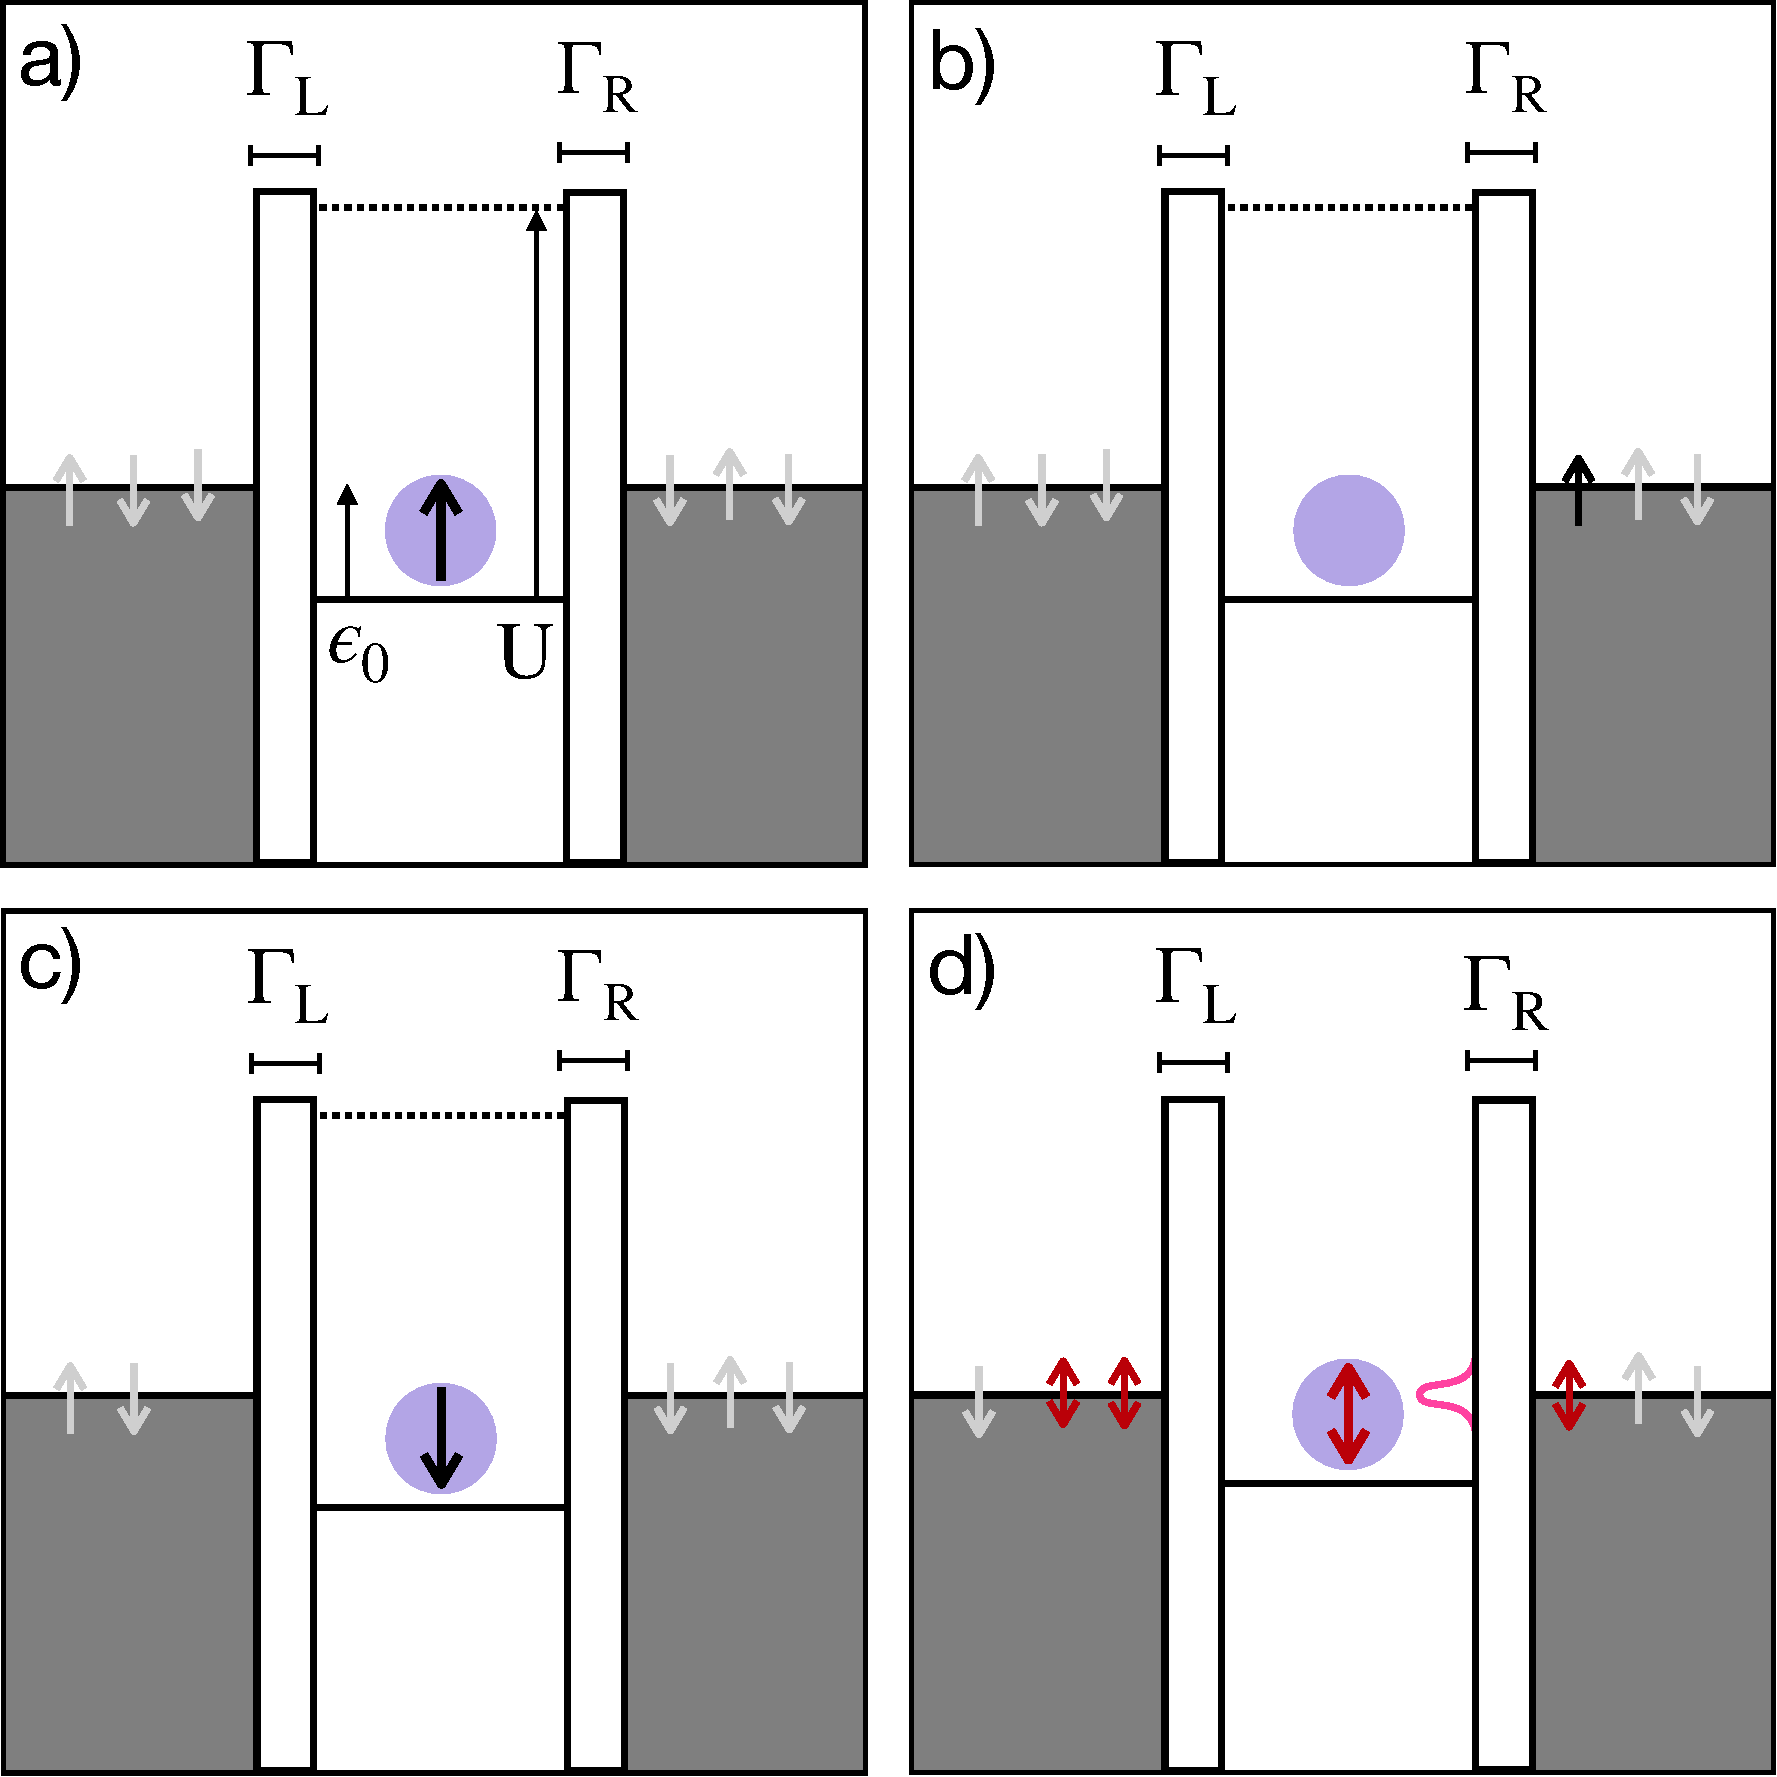
\includegraphics[width=0.75\textwidth]{figures/ch2/figure11.pdf}
\caption[Kondo Effect Illustration : Quantum Dot]{\label{fig:ch2/kondo_dot_diagram} 
% For some options that work with pdf\LaTeX, please see this discussion:
%\url{http://tex.stackexchange.com/questions/11839}. 
Coulomb blockade energy diagram illustrates the formation of a Kondo singlet in a quantum dot. Here, the dot acts as a localised spin. The dark grey represents the continuous energy level of electrons in the leads. The white rectangles represent tunnel barriers between the quantum dot and leads. The rate of tunnelling is denoted by the parameter $\Gamma$; the wider (narrower) the barrier, the smaller (larger) the rate of tunnelling. (\textbf{a}) The quantum dot has a one-spin degenerate energy level with dot energy $\mathrm{\epsilon_0}$, occupied by a single electron. The charging energy, $\mathrm{U}$, separates the next energy level. According to Fig.~\ref{fig:ch1/dot_intro}, zero conductance is expected through the quantum dot. However, (\textbf{b},\textbf{c}) depict a possible virtual tunnelling event. Here, the spin-up electron tunnels out of the dot, and a spin-down electron tunnels into the dot within a short time. (\textbf{d}) Many virtual tunnelling events involving possible spin flips lead to a correlated state, the Kondo singlet. This state is pictured as a narrow density of states formed at the Fermi energy of the leads. If a Kondo singlet has been formed, enhanced conductance is measured through the quantum dot, even as the dot energy $\epsilon_0$ is below the energy level of the leads. Note the formation of the Kondo singlet requires an odd number of electrons in the quantum dot.
 }
 \end{center}
\end{figure}


Until the late 1990s, theorists primarily explored the Kondo effect due to the difficulty of experimentally controlling the Kondo state~\cite{still_irresistible,kondo_review}. However, after advances in quantum dot design, the potential for precise in-situ control was irresistible, and the first measurement of a Kondo singlet was in 1998~\cite{goldhaber_first_kondo}. Around this time a scanning tunneling microscope (STM) was also used to study the Kondo effect~\cite{stm_kondo}.

In quantum dots, an odd number of electrons results in an unpaired electron that acts as the magnetic impurity in bulk metals. Like bulk metals, the conduction electrons in the 2DEG can interact with the net spin in the quantum dot. The advantage of studying the Kondo effect in quantum dots comes from the in-situ control over the coupling strength, voltage bias, and energy level of the magnetic impurity.

The formation of a Kondo singlet in quantum dots is shown in Fig.~\ref{fig:ch2/kondo_dot_diagram}. 
Suppose the dot energy of the quantum dot is far below the Fermi energy of the leads. In that case, the electron is not expected to tunnel out of the dot as it does not have the required energy to reach the available empty energy levels in the leads (Fig.~\ref{fig:ch1/dot_intro}). However, a second-order tunnelling process can occur resulting in a non-zero conductance, even as the dot energy is below the Fermi energy of the leads. If the electron in the quantum dot tunnels into the leads (Fig.~\ref{fig:ch2/kondo_dot_diagram}\textbf{b}) another electron must tunnel into the quantum dot within a timescale limited by Heisenberg’s uncertainty principle (Fig.~\ref{fig:ch2/kondo_dot_diagram}\textbf{c}). This second-order process can result in a spin flip of the impurity. Many of these virtual tunnelling events will lead to the formation of a singlet state illustrated in Fig.~\ref{fig:ch2/kondo_dot_diagram}\textbf{d}. This results in a narrow density of states formed at the Fermi energy of the leads. 


 \begin{figure}[!hbt]
 \begin{center}
%% includegraphics: comment the following if not using the graphicx package
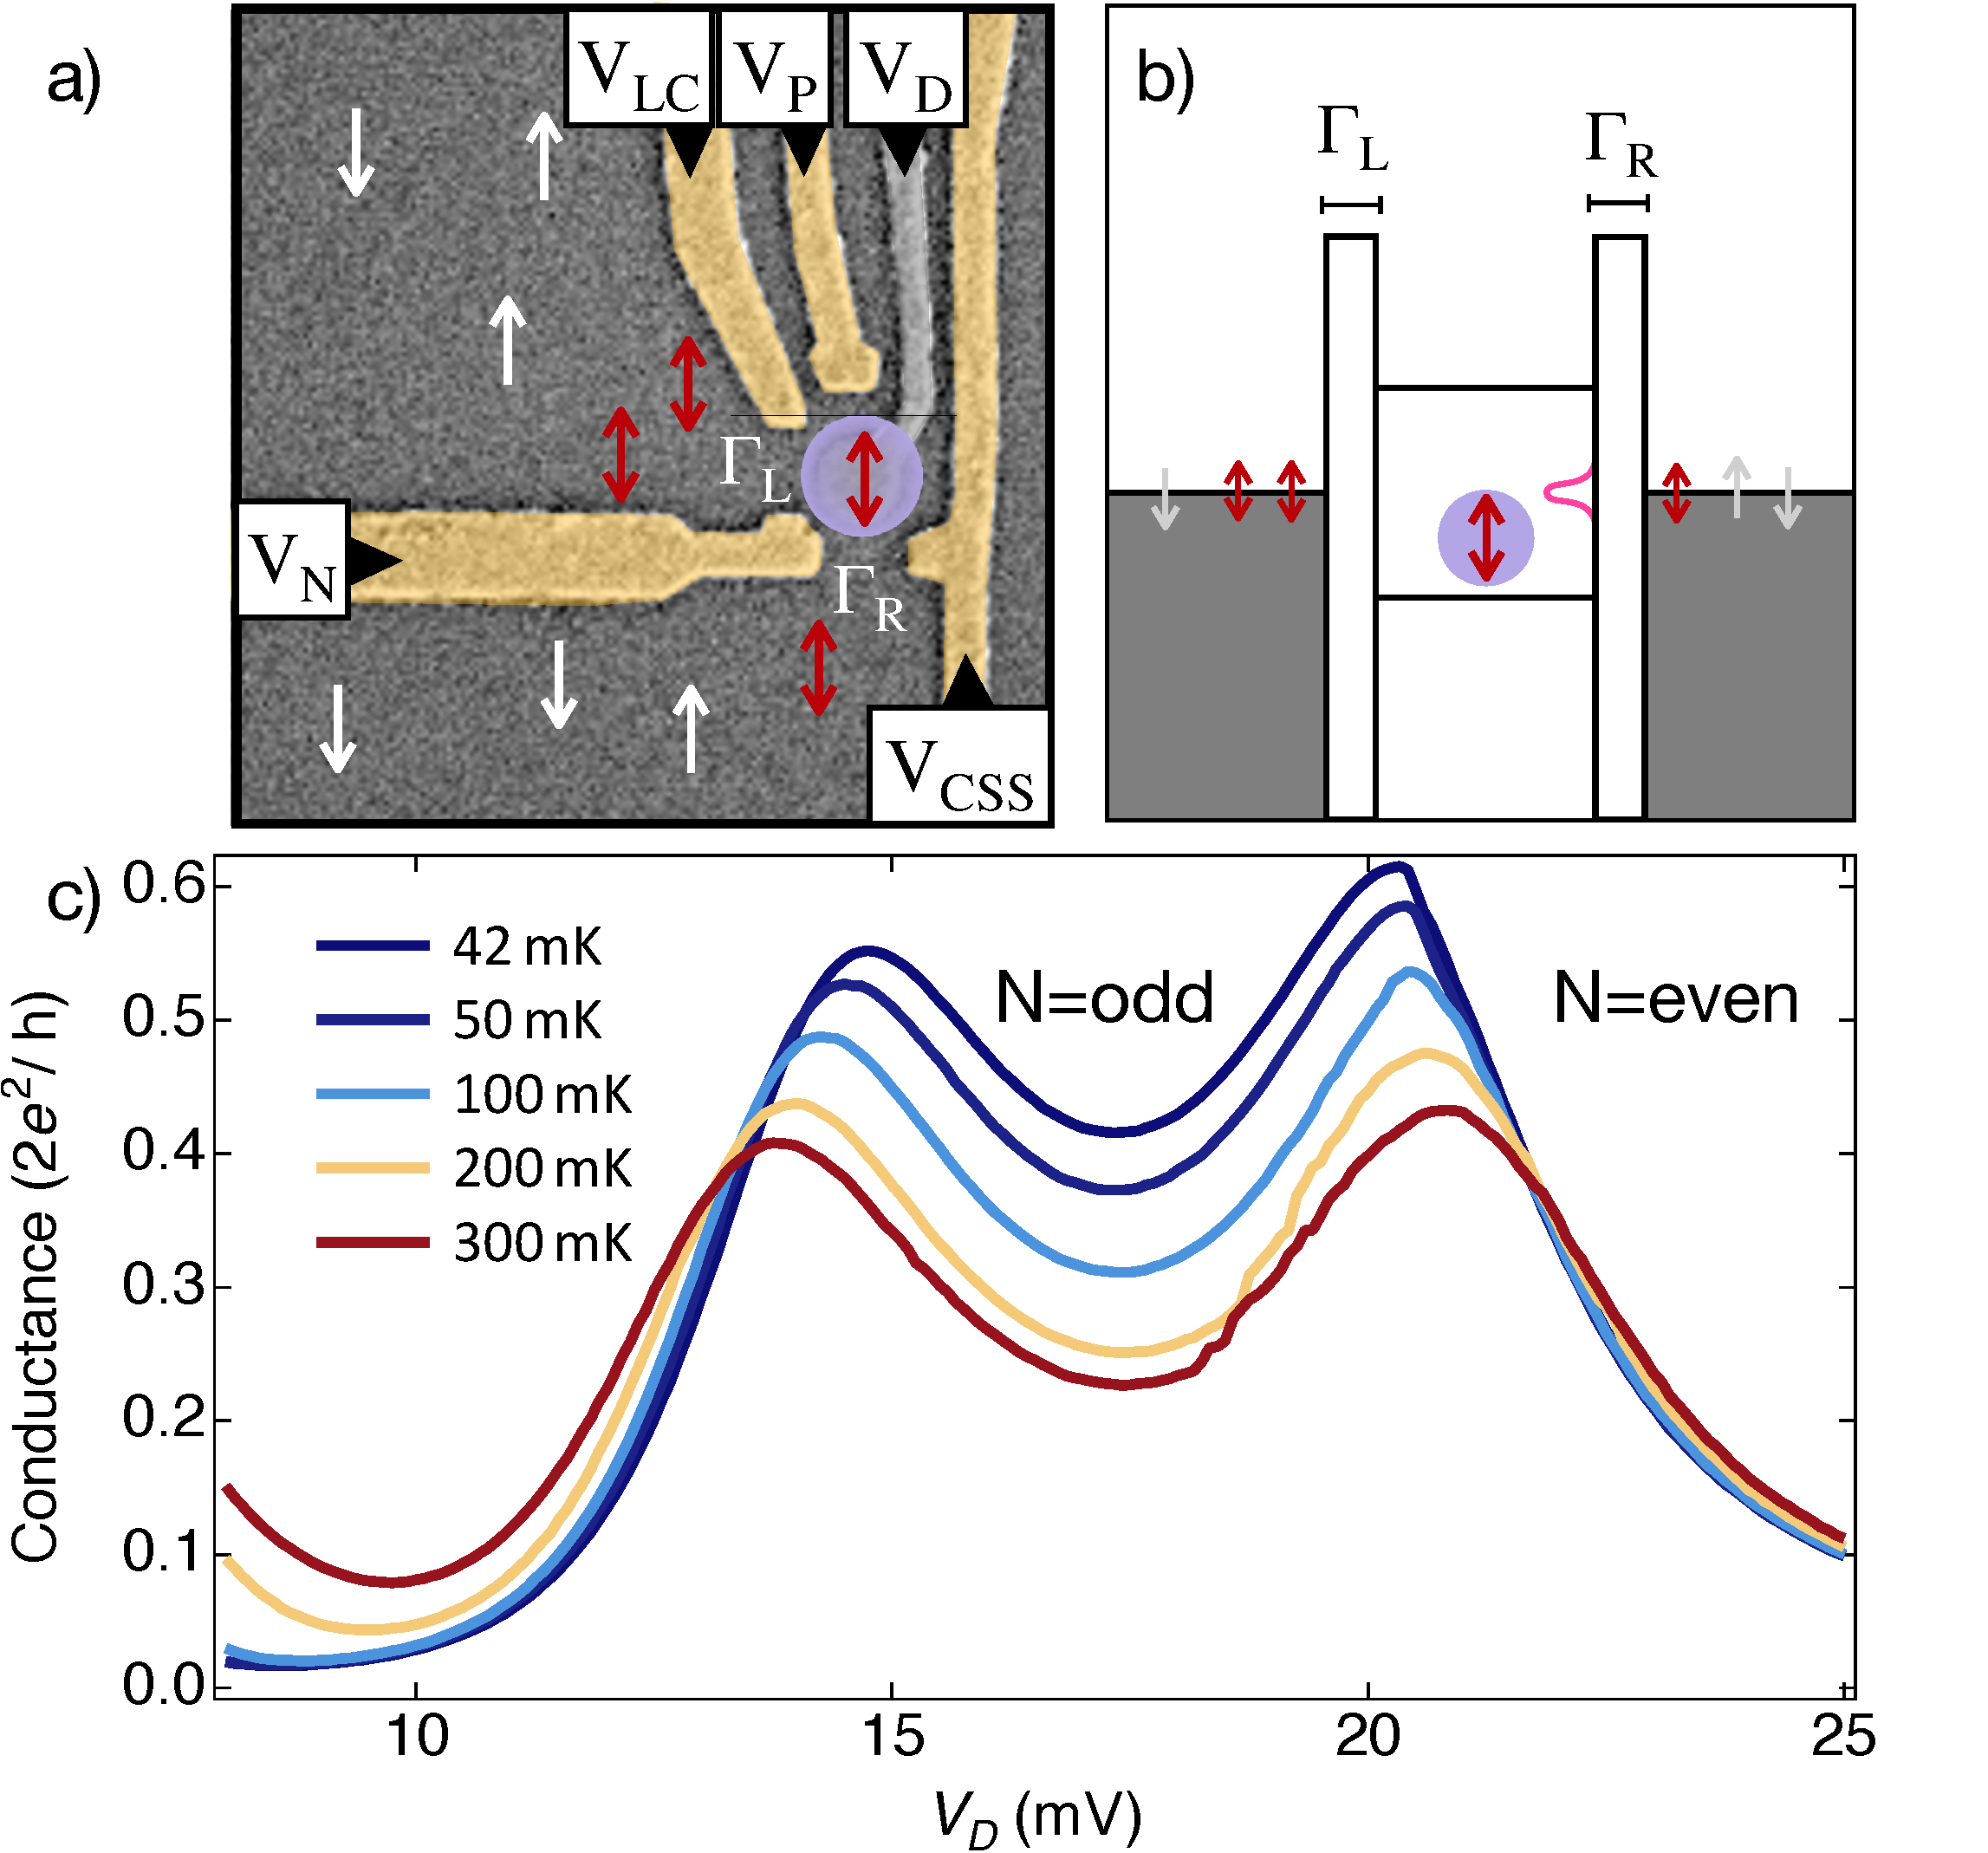
\includegraphics[width=0.9\textwidth]{figures/ch2/figure12.pdf}
\caption[Kondo Effect in a Strongly Coupled Quantum Dot]{\label{fig:ch2/kondo_regime_conductance} 
% For some options that work with pdf\LaTeX, please see this discussion:
%\url{http://tex.stackexchange.com/questions/11839}. 
(\textbf{a}) SEM image of the gates used to define a quantum dot. The dot contains an odd number of electrons, and the tunnel barriers are tuned to form a Kondo singlet. (\textbf{b}) Coulomb blockade energy diagram picture of a Kondo singlet. As the dot energy falls below the energy level of the leads, there is enhanced conductance due to virtual tunnelling events through the quantum dot. (\textbf{c}) Data showing the temperature dependence of conductance through a quantum dot when a Kondo singlet is formed. In the even occupied sides, conductance decreases as the temperature is lowered. With odd occupation, a Kondo singlet forms, and conductance increases with decreasing temperature.}
 \end{center}
\end{figure}



 Unlike the resistivity increase in bulk metals, the presence of a Kondo singlet leads to enhanced conductance through the quantum dot. Figure~\ref{fig:ch2/kondo_regime_conductance}\textbf{c} shows a measurement of conductance at a range of temperatures. At odd occupation, a Kondo singlet is formed and conductance through the quantum dot increases with decreasing temperature. This enhancement of conductance is dependent on a single parameter which sets the energy scale, the Kondo temperature $\mathrm{T_K}$. The Kondo temperature is given by Haldane~\cite{Haldane1978, kondo_thesis_stuttgart} as,
 

\begin{equation}\label{eq:kondo_temp}
 \mathrm{T_K} = 
 \frac{\sqrt{\hbar\Gamma \mathrm{U}}}{2\mathrm{k_B}}
 e^{\pi \epsilon_0 (\epsilon_0 + \mathrm{U})/\hbar\Gamma\mathrm{U}}
\end{equation}

 \noindent Here $\epsilon_0$ is the dot energy, $\mathrm{U}$ the charging energy and $\Gamma$ is the coupling of the dot to both source and drain leads, $\mathrm{\Gamma = \Gamma_L + \Gamma_R}$. 
 An important realisation from Eq.~\ref{eq:kondo_temp}, is that the Kondo temperature is not a constant value but is dependent on parameters that can be controlled in an experiment. 
 In Fig.~\ref{fig:ch2/kondo_regime_conductance}\textbf{a}, the dot energy is controlled by V\textsubscript{P} or V\textsubscript{D} and the coupling by V\textsubscript{LC}, V\textsubscript{N} or V\textsubscript{CSS}.
The expression for the Kondo temperature in Eq.~\ref{eq:kondo_temp}, only holds in the `Kondo regime'. The Kondo regime is characterised by $\tilde{\epsilon}_0<<-0.5$ where $\tilde{\epsilon}\equiv \epsilon_0/\Gamma$. Qualitatively, this regime is satisfied when the full charge of the electron is in the quantum dot. Consequently, as the dot energy is raised so that only a fraction of the electron charge is localised in the quantum dot, this expression for the Kondo temperature breaks down. However, the quantum dot still mainly exhibits a net spin, and Kondo enhancement remains. Importantly, the Kondo temperature increases as the dot energy approaches the Fermi energy of the leads~\cite{goldhaber_mv}, although it may not be exponential in form. This `turning on' of the Kondo effect close to the Fermi energy of the leads is the basis for measurements in the following Chapter~\ref{cha:mixed_valence_conductance}.
 

Many early measurements on the Kondo effect in quantum dots used very strong couplings, so the system temperature remained below the Kondo temperature deep into the Kondo regime~\cite{kondo_unitary}. Such studies examined temperature dependence of the conductance in the Coulomb blockade valley where the conductance dependence on temperature is non-monotonic and has a minimum at finite temperatures~\cite{Pustilnik2004}. The Kondo temperature (Eq.~\ref{eq:kondo_temp}) sets a new many-body scale in the Kondo regime. The Kondo temperature can be used to normalise the conductance such that it is independent of other energy scales $\Gamma$, $\mathrm{U}$, and $\tilde{\epsilon}_0$~\cite{costi_kondo_mv_eo_regime}. This normalisation is given as, 

\begin{equation}\label{eq:kondo_conductance}
 \mathrm{G(T)} =
 \mathrm{G_0}
 \left(
 \frac{\mathrm{T_K'^{2}}}{\mathrm{T^2} + \mathrm{T_K'^{2}}}
 \right)^\mathrm{s}
\end{equation}

\noindent Here $\mathrm{T_K'^{2}} = \mathrm{T_K}/\sqrt{2^{\mathrm{1/s}}-1}$ and $\mathrm{s} \approx 0.20$ for a spin 1/2 system in the Kondo regime~\cite{goldhaber_mv}. The parameter $\mathrm{s}$ determines the steepness of the conductance drop with increasing temperature. The one-parameter scaling of the conductance in the Kondo regime is used as one of the demonstrations of the Kondo effect. Other measurements include a zero bias peak in the Coulomb blockade valley~\cite{kondo_unitary} and a splitting of this zero bias peak with magnetic field~\cite{cronenwett_tunable_kondo}. 

Other efforts have been made to explore the Kondo effect with less strong coupling. In this regime, the conductance in the middle of the Coulomb blockade valley does not increase with decreasing temperature~\cite{goldhaber_mv}. However, the dot energy of the quantum dot can be tuned to increase the Kondo temperature. As the dot energy approaches the Fermi energy of the leads, a conductance enhancement due to the Kondo effect can be recovered at sufficiently low system temperatures. The next Chapter~\ref{cha:mixed_valence_conductance} will focus on this regime of weaker coupling.



\chapter[Occupation Resolved Conductance of the Kondo Effect]{Occupation Resolved Conductance of the Kondo Effect}\label{cha:mixed_valence_conductance}
% Probably should be called: Occupation resolved conductance of the Kondo effect

\epigraph{Po bitvě je každý generál.}{Czech proverb}%~\cite{Strauss1998}}

\noindent To my knowledge, the following work in this chapter is the first time that conductance and charge transitions have been simultaneously measured to resolve the conductance enhancement due to the Kondo effect as a function of the occupation in an experiment. The conductance enhancement from Kondo is most pronounced when the quantum dot is strongly coupled ($\mathrm{\Gamma/k_BT}>>1$) to the source and drain leads. Previous measurements of the Kondo effect focus on the conductance enhancement between Coulomb peaks. However, when the coupling is strong, charge transitions broaden and become challenging to convert into an occupation. The following work falls between the tightly confined window of strong coupling to see the Kondo effect and weak coupling, where charge transitions are easily measured. 

\section{Introduction}
Previous measurements of the Kondo effect in quantum dots study the temperature dependence of conductance between Coulomb peaks. It is in this so-called Kondo regime that the full charge of the electron is in the dot, so there is a definite net spin, and the theory is well understood~\cite{costi_kondo_mv_eo_regime, kondo_unitary}. In this regime, the Kondo temperature (Eq.~\ref{eq:kondo_temp}) sets a new, many-body scale and is used to universally scale the conductance (Eq.~\ref{eq:kondo_conductance}). This one-parameter scaling of conductance in the Kondo regime is used as one of the demonstrations of the Kondo effect. When the coupling between the quantum dot and source and drain leads is reduced, the Kondo temperature drops below the system temperature, and the conductance enhancement is not seen between Coulomb peaks. Only a handful of experiments have studied conductance with less strong coupling~\cite{goldhaber_mv}. Such studies observed the parameter $\mathrm{s}$ from Eq.~\ref{eq:kondo_conductance} and found that in the Kondo regime (the full charge of the electron is in the dot), $\mathrm{s}$ was constant and equal to $0.20$. However, as the shoulder of a Coulomb peak was approached ($\tilde{\epsilon}_0>-0.5$), $\mathrm{s}$ varied rapidly. Qualitatively, this regime is entered when the dot energy $\epsilon_0$ approaches the Fermi energy of the leads, and only a fraction of the electron charge is in the dot. 


Our aim was to measure the Kondo effect with a coupling strength such that the conductance between Coulomb peaks was zero. This regime, characterised by a relatively small $\Gamma$, results in a small Kondo temperature between Coulomb peaks, and no conductance enhancement would be measured. However, the Kondo temperature will increase as the dot energy approaches the Fermi energy of the leads (moves towards the shoulder of a Coulomb peak). Hence, for relatively small coupling strengths, the Kondo effect can still be seen as a very small conductance enhancement on the odd occupied side of a Coulomb peak. As the conductance enhancement in this regime is very small, it is insufficient to investigate the Kondo effect with a conductance measurement only, for two reasons. Firstly, entropy shifts the occupation of the quantum dot with temperature. This effect has been taken advantage of in a recently developed entropy measurement technique~\cite{hartman, child_strong, child_meas}. This shift in occupation can be ignored when the coupling is strong, and conductance enhancement between Coulomb peaks is large. Secondly, charge motion in the dopant layer can shift the conductance left or right with respect to the gate voltage in a scan. The shifting from charge motion renders it impossible to offset the effects of entropy by retroactively shifting conductance. 

For these two reasons, it is necessary to simultaneously measure a second `reference' signal alongside the conductance. This reference signal can then be used to offset the above effects and allow for comparison of the conductance across multiple temperatures. We measure the charge in the quantum dot simultaneously with conductance. Assuming a linear relation between the measured change in charge and the real occupation of the quantum dot, the charge transition is converted into an occupation. The occupation is then used to plot the conductance as a function of occupation. A shifting of the conductance maximum to a higher occupation is a signature of the Kondo effect. 
As the universal scaling of conductance does not hold in this regime, a comparison to theory calculations (described in an upcoming section) is required to verify Kondo enhancement. 





\section{Occupation Resolved Conductance Method}
The conductance and charge of the quantum dot are simultaneously measured to investigate the small enhancement of conductance due to the Kondo effect with relatively small coupling. On the hardware side, a simultaneous measurement of the charge and conductance is trivial as two different current amplifiers are simply connected to the device. 
The first current amplifier measures the conductance through the quantum dot and the other, current through the charge sensor. Each current amplifier is connected to two analog-to-digital converters (ADCs), which sample data points simultaneously. 
Conductance is measured using a pseudo-lockin technique. Here a DAC channel voltage biases the current amplifier using a \qty{\pm1}{\micro V} square wave. The underlying signal is recovered in analysis by multiplying with a sine wave of equal frequency and averaging all the points per square wave cycle. This technique mitigates the effects of bias drift in the current amplifier so that a reliable \qty{1}{\micro V} source-drain bias is applied across the dot. 
A \qty{100}{\micro V} DC bias is applied across the charge sensor. Large source-drain bias across the charge sensor can de-phase the Kondo singlet~\cite{kondo_controlled_dephasing}, however, a range of 50-\qty{250}{\micro V} source-drain biases was tested with no significant effect.

It is much trickier to tune the quantum dot into a regime where both the conductance and charge transition can be compared to theory. When weakly coupled ($\mathrm{\Gamma/k_BT}<<1$), the charge transitions have a sharp drop in current and can be fit analytically using Eq.~\ref{eq:cs_lineshape}. However, a weakly coupled Coulomb peaks amplitude drops with the strength of coupling~\cite{Kouwenhoven_1997_electron_transport} as,


\begin{equation}\label{eq:cond_amp}
 \mathrm{G_0} \propto
 \frac{\Gamma_\mathrm{L}\cdot\Gamma_\mathrm{R}}{\Gamma_\mathrm{L}+\Gamma_\mathrm{R}}
\end{equation}


\noindent where $\mathrm{G_0}$ is the conductance maximum. This decrease in conductance amplitude means that the conductance signal can be lost within the background noise. Additionally, as the Kondo temperature decreases with reduced coupling, the conductance enhancement due to Kondo can become immeasurable.


Alternatively, in a strongly coupled regime ($\mathrm{\Gamma/k_BT}>>1$), Coulomb peaks are usually easier to measure. Here the line shape for a Coulomb peak is given by the Breit-Wigner formula~\cite{Breit1936}. The conductance is maximum when the dot energy is in line with the Fermi energy of the leads and depends on the coupling as 

\begin{equation}\label{eq:cond_amp_strong}
 \mathrm{G_0} \propto
 \frac{\Gamma_\mathrm{L}\cdot\Gamma_\mathrm{R}}{\left(\Gamma_\mathrm{L}+\Gamma_\mathrm{R}\right)^2}
\end{equation}

\noindent In both weakly and strongly coupled regimes, it is evident that the conductance reaches a maximum when the tunnel barriers are symmetric ($\Gamma_\mathrm{L}=\Gamma_\mathrm{R}$). Strong coupling also has the added benefit of an increase in Kondo temperature, leading to greater enhanced conductance. 
However, as Coulomb peaks become easier to measure, charge transitions become very broadened and difficult to measure (Fig.~\ref{fig:ch1/virtual_gate_example}). When strongly coupled, large sweeps in gate voltage are required to cover a range where the quantum dot is fully unoccupied to occupied. This can result in the charge sensor being pushed into a non-linear regime due to the cross-capacitive coupling from the sweep gate.
A non-linear relationship between the current through the charge sensor and the addition of charge into the quantum dot makes extraction of dot occupation from the charge transition unreliable. Hence, a virtual gate shown in Fig.~\ref{fig:ch1/virtual_gate_example}, that keeps the current through the charge sensor constant is required. The exact ratio of gates used to form a virtual gate can drastically change the underlying shape of the charge transition, which will be discussed in an upcoming section. 


\subsection{Numerical Renormalisation Group (NRG)}
The dot is carefully tuned to a coupling regime where the conductance enhancement due to Kondo is expected, and charge transitions are reliably measured. As previous tests of the Kondo effect are not possible in this regime, a comparison to Numerical Renormalisation Group (NRG) calculations~\cite{nrg} is required. Our theory collaborators (Yigal Meir, Yaakov Kleeorin, and Andrew Mitchell) provide these calculations. 
Two 2D datasets corresponding to conductance and occupation are received.The columns are energy scaled by $\Gamma$ (energy/$\Gamma$), so the x-axis is unitless. The rows in the 2D datasets correspond to a different $\mathrm{\Gamma/k_BT}$ value. We confirmed with Yaakov that the lineshape does not change if both $\mathrm{T}$ and $\mathrm{\Gamma}$ increase together. The lineshape represents the ratio $\mathrm{\Gamma/k_BT}$, not $\mathrm{\Gamma}$ or $\mathrm{T}$ individually.

To compare NRG to data, $\mathrm{\Gamma/k_BT}$ should be reliably determined so the correct row from NRG is used. Then, the correct scaling is applied to convert the NRG into measurement units. Conductance and charge transitions have similar scaling parameters. Amplitude, x-offset and lever arm which scales the NRG x-axis in units of mV. The occupation NRG has extra parameters: a y-offset, which comes from the current through the charge sensor; a linear term, which comes from the cross-capacitance between the sweep gate and charge sensor; and an occupation-dependent linear term. 
This occupation-dependent linear term reflects a change in the cross-capacitance as an electron enters the quantum dot. In Fig.~\ref{fig:ch3/cond_occ_QPC_vs_ct}, the charge transition slopes are different between the unoccupied (left) and occupied (right) sides. We argue that the additional charge of an electron in the quantum dot can give rise to such a change in cross-capacitance. Many of these parameters have low cross-correlation when fitting data to NRG, meaning the global minimum of the minimiser is reliably reached. However, this is not true for the parameters $\mathrm{\Gamma/k_BT}$ and lever arm. Changes to $\mathrm{\Gamma/k_BT}$ can be offset by a change in lever arm, and fitting a single trace allowing both parameters ($\mathrm{\Gamma/k_BT}$ and lever arm) to vary freely is unreliable. 


\subsection{Conductance Global Fit to NRG}
In the temperature broadened regime ($\mathrm{\Gamma/k_BT} < 1$), $\mathrm{\Gamma/k_BT}$ and lever arm are decoupled as the broadening of the conductance or charge transition is from temperature only. To access the temperature broadened regime from the gamma broadened regime ($\mathrm{\Gamma/k_BT} > 1$), the temperature of the fridge is increased until $\mathrm{\Gamma/k_BT} \lesssim 1$. Figure~\ref{fig:ch3/cond_ct_gf} shows that data is taken at multiple temperature setpoints across this range so that $\mathrm{\Gamma/k_BT}$ and lever arm can be reliably determined. Conductance and charge transitions are simultaneously measured at each temperature. However, only the conductance data is used to determine $\mathrm{\Gamma/k_BT}$ and lever arm, as it is generally cleaner. A global fit to the conductance data, including each temperature setpoint, is used in Fig.~\ref{fig:ch3/cond_ct_gf}\textbf{a}. Here $\mathrm{\Gamma}$ and lever arm are allowed to vary, but held fixed between temperatures, and $\mathrm{T}$ is held fixed to the calculated electron temperatures from Fig.~\ref{fig:ch1/electron_temp}. The other parameters (amplitude and x-offset) used to fit the NRG to conductance data are allowed to vary freely.
The fitting range is the full width at $90\%$ the maximum conductance. This removes any bias of picking a `good' fitting range. 

\subsection{Charge Transition Fit to NRG}
Each charge transition is fit separately to NRG, where $\mathrm{\Gamma/k_BT}$ and lever arm determined from the conductance global fit, are held fixed. All other parameters (amplitude, x-offset, y-offset, linear and occupation-dependent linear) are allowed to vary freely (Fig.~\ref{fig:ch3/cond_ct_gf}\textbf{b}). The fitting range of the charge transitions is maximised up to, but excluding charge jumps.


\begin{figure}[H]
 \begin{center}
%% includegraphics: comment the following if not using the graphicx package
 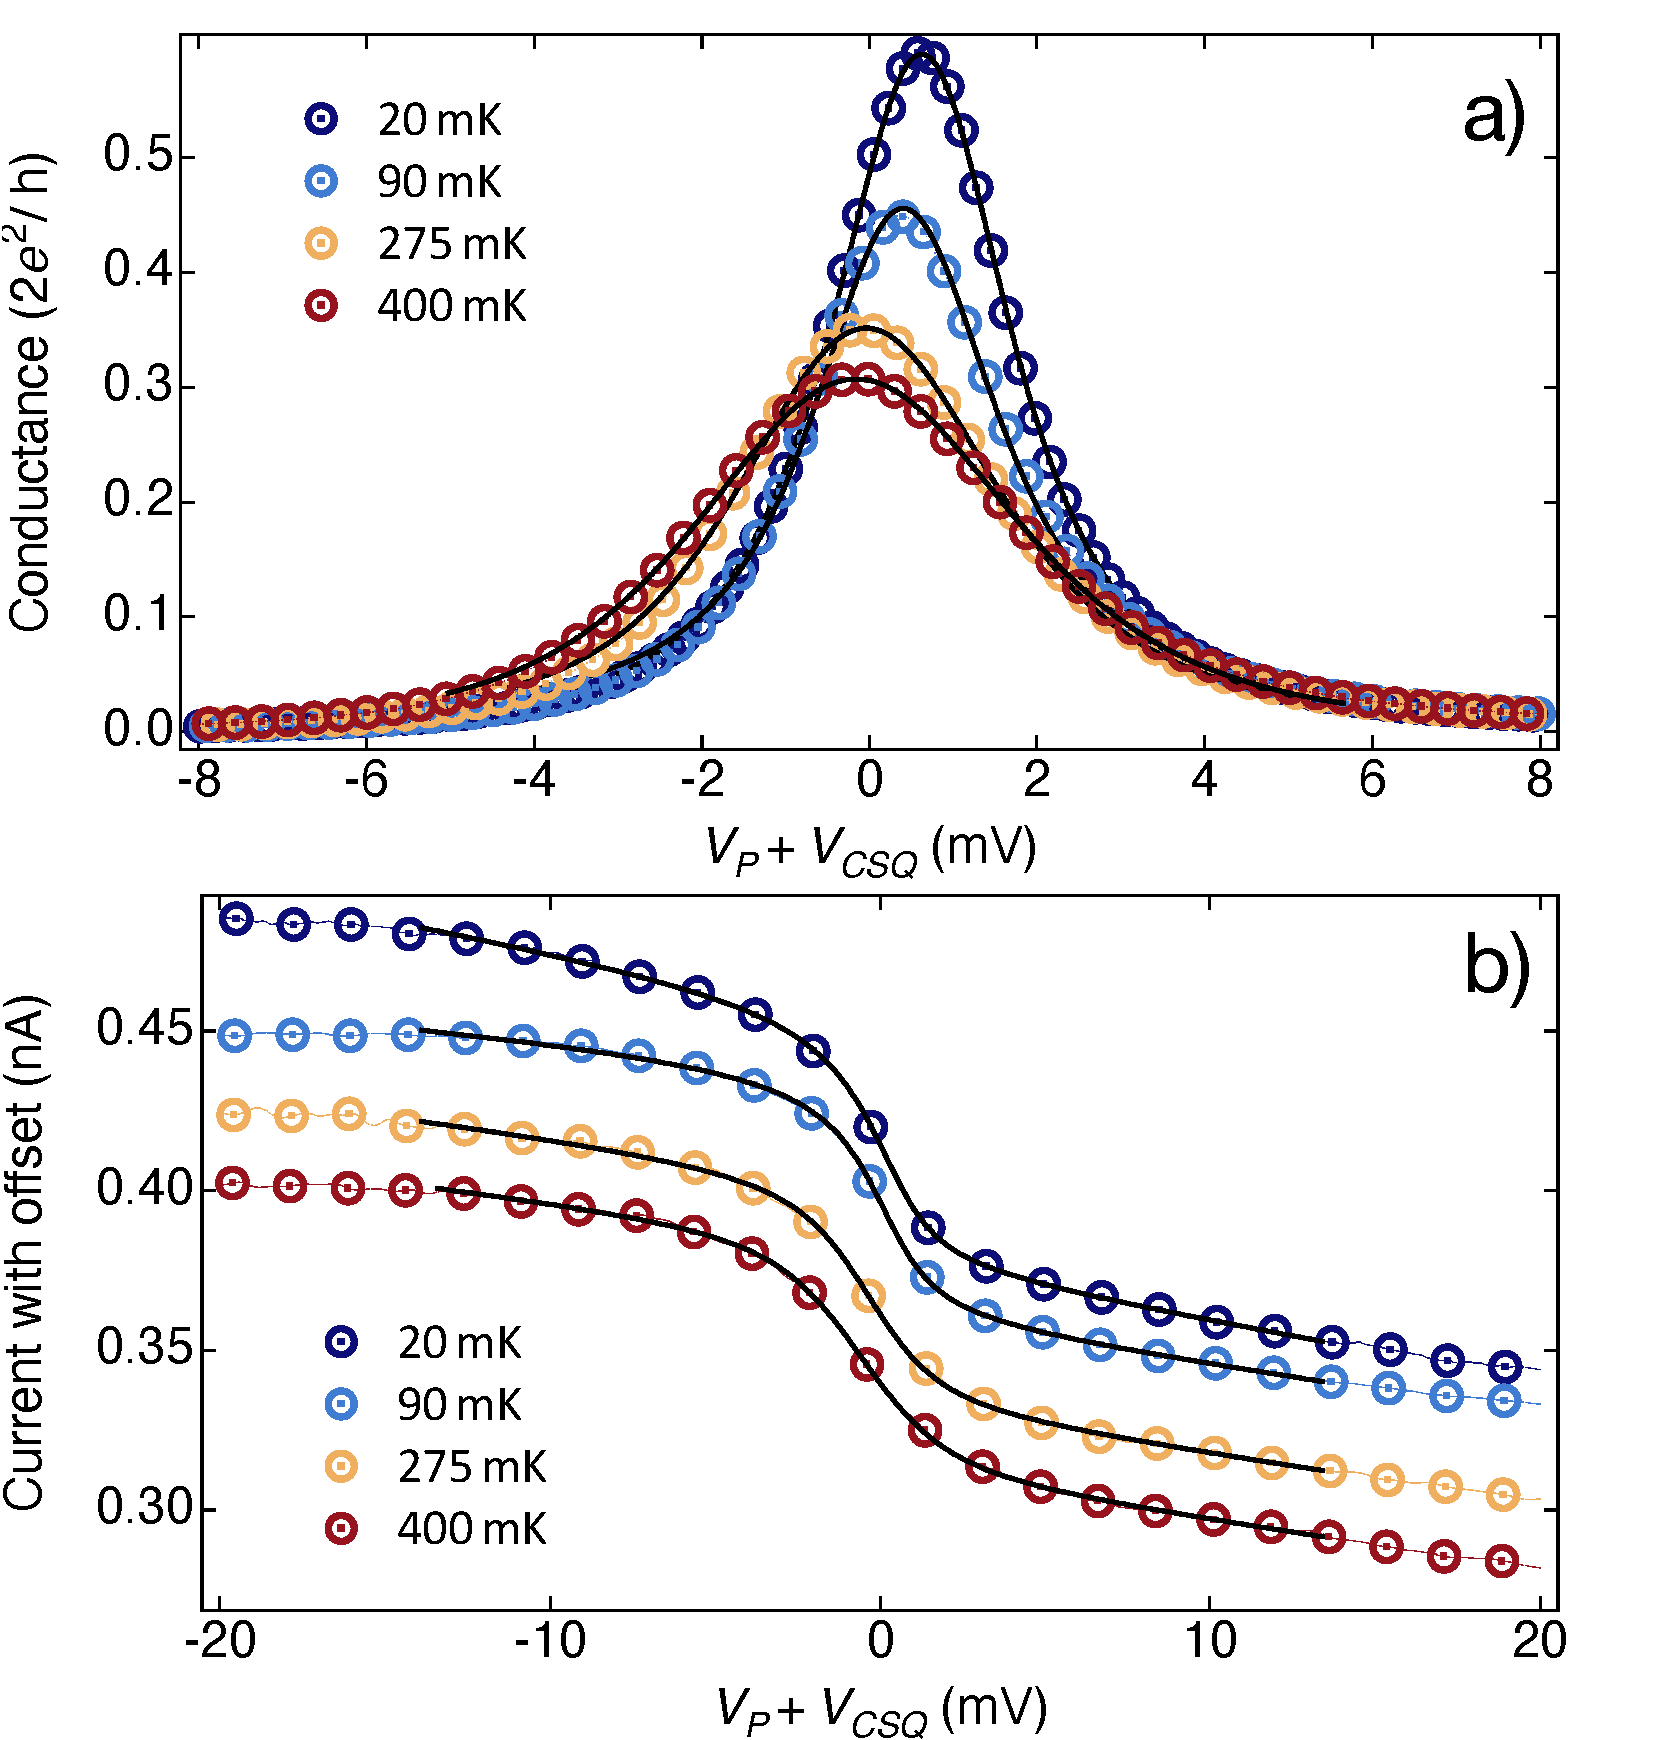
\includegraphics[width=0.85\textwidth]{figures/ch3/figure13.pdf}
 \caption[Fit Conductance and Charge Transition to NRG]{\label{fig:ch3/cond_ct_gf} 
 % For some options that work with pdf\LaTeX, please see this discussion:
 % \url{http://tex.stackexchange.com/questions/11839}. 
 (\textbf{a}) Conductance as a single electron enters a strongly coupled ($\mathrm{\Gamma/k_BT > 1}$) quantum dot at four different temperatures. The x-location of the conductance maximum has not been shifted and is the original x-location of the measured data. The fits (in grey) are from a global fit to NRG, where the $\Gamma$ and lever arm parameters are held fixed across all four temperatures. (\textbf{b}) Charge transitions are measured simultaneously with the conductance. Each charge transition is separately fit to NRG, where the $\Gamma$ and lever arm parameters are held fixed to the values determined from the global fit to conductance.}
 \end{center}
\end{figure}



% \newpage

\subsection{Determining Occupation}

\begin{figure}[!hbt]
 \begin{center}
 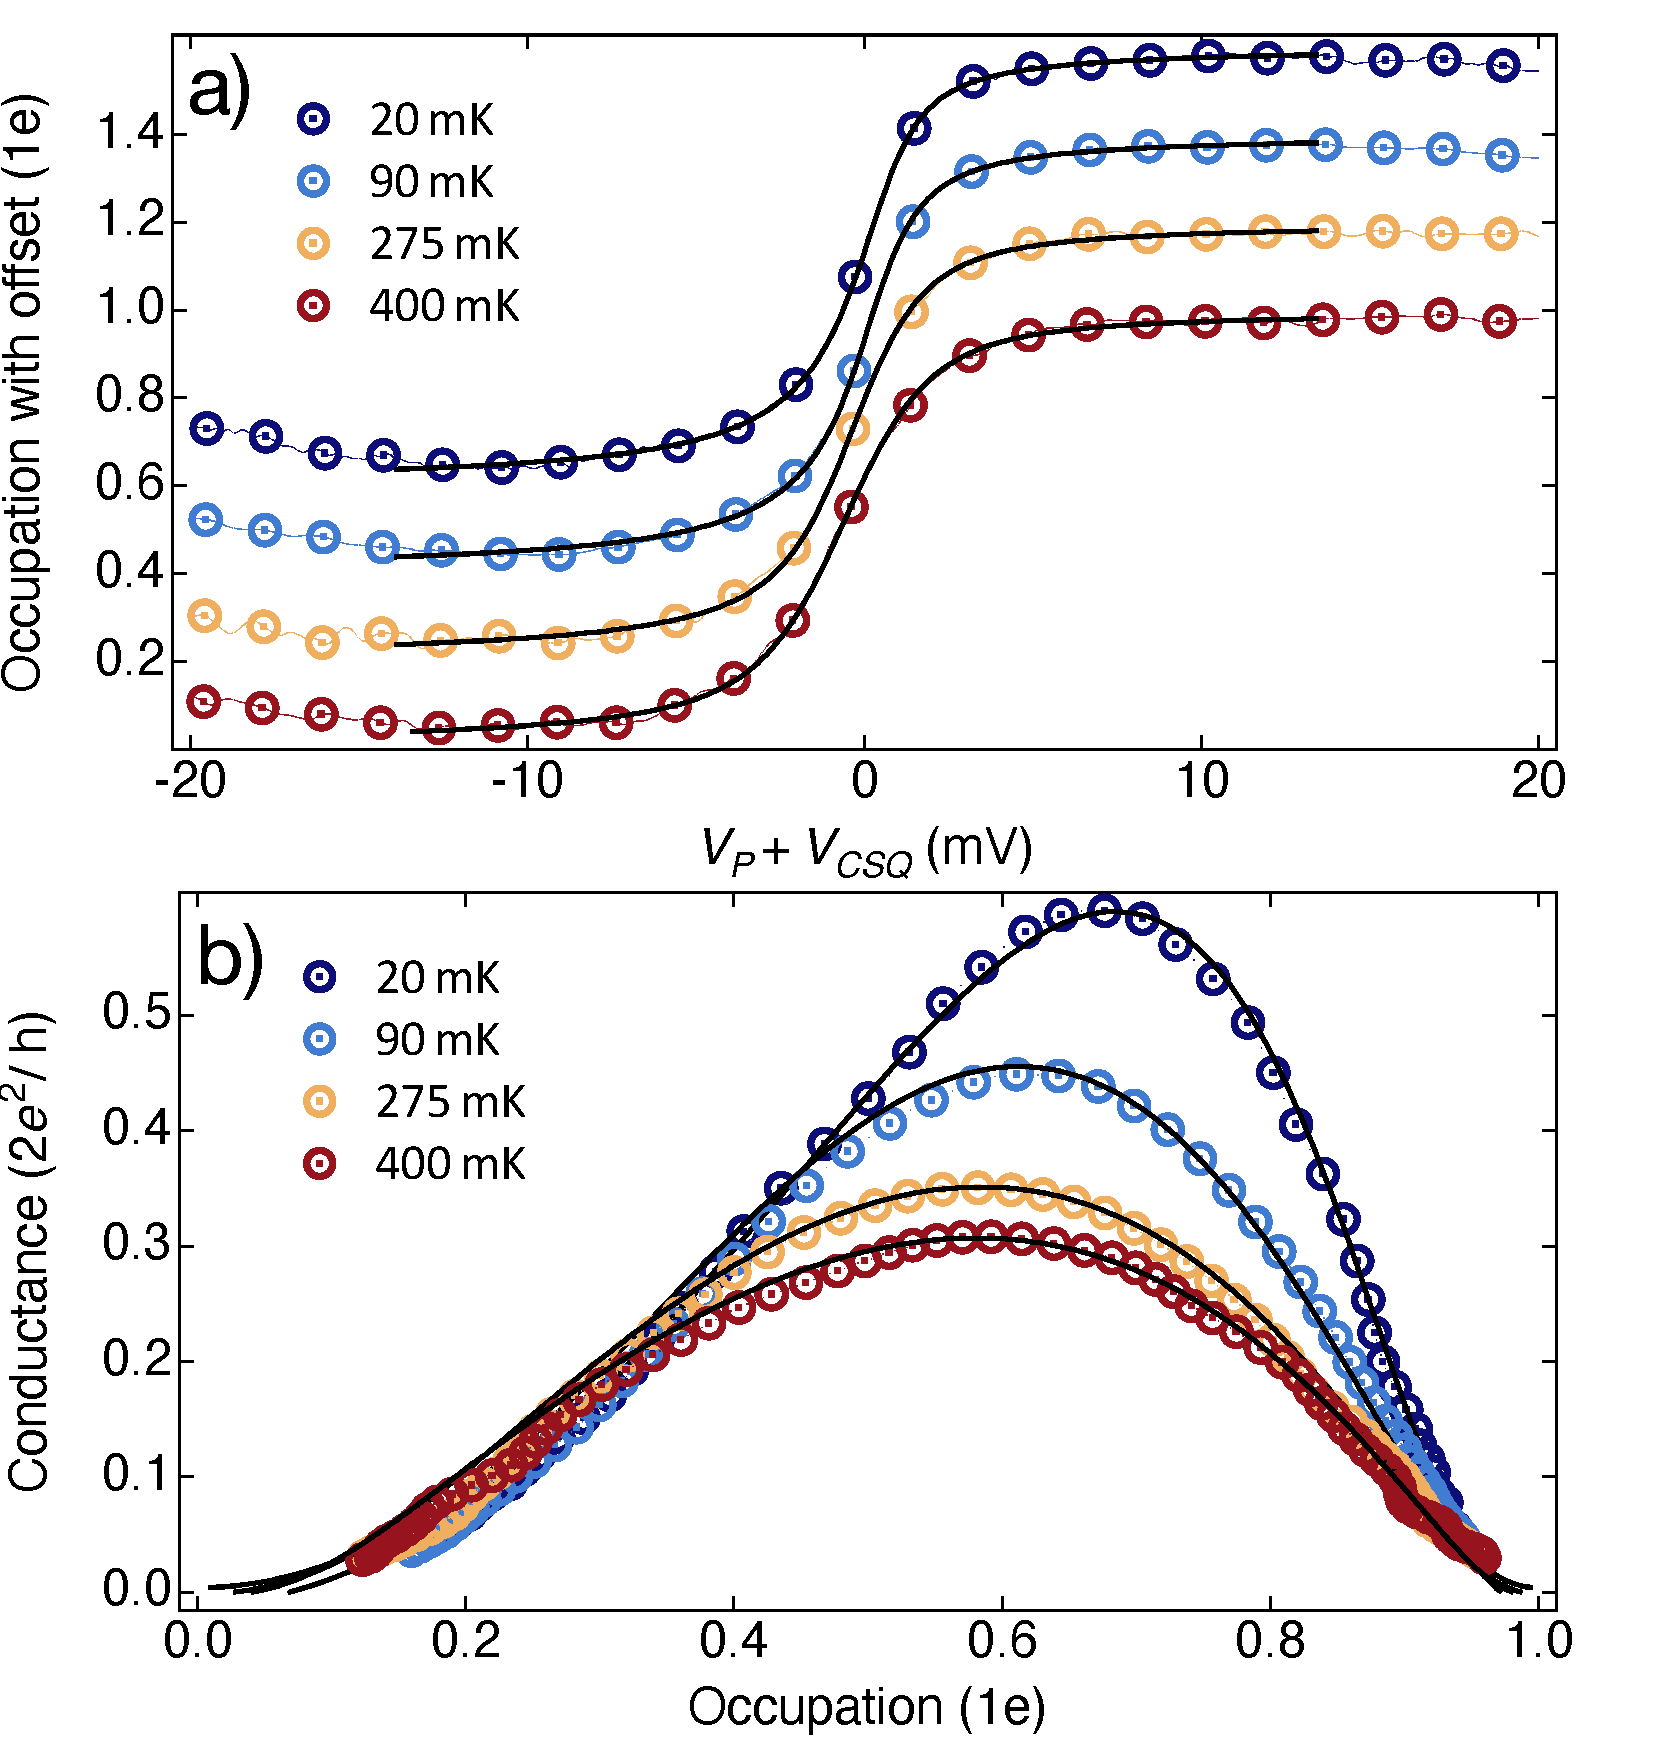
\includegraphics[width=0.85\textwidth]{figures/ch3/figure14.pdf}
 \caption[Conductance versus Occupation : Varying Temperature]{\label{fig:ch3/cond_vs_occ_gf} 
 % For some options that work with pdf\LaTeX, please see this discussion:
 % \url{http://tex.stackexchange.com/questions/11839}. 
 (\textbf{a}) Charge transitions are converted to occupation by removing the relevant fit parameters. These are amplitude, current offset, cross-capacitance of virtual gate, and occupation-dependent cross-capacitance. (\textbf{b}) Conductance versus occupation is used to show the enhanced conductance due to Kondo. As temperature decreases, the conductance maximum occurs at greater occupation. The NRG (grey) conductance versus occupation corresponding to the determined $\mathrm{\Gamma/k_BT}$ is plotted on top of the data, where good agreement is found at each temperature.}
 \end{center}
\end{figure}


The charge transition cannot be used as a reference to compare with conductance due to changing amplitude and linear terms with changes in dot settings. However, charge transitions can be converted into an occupation, allowing for the comparison of conductance enhancement between dot settings. The fit parameters from the NRG fit to the charge transitions are used to remove relevant terms. The current offset (y-offset) and linear term are removed trivially. The occupation-dependent linear term is removed by multiplying this linear term with the correct NRG occupation row corresponding to $\mathrm{\Gamma/k_BT}$. Lastly, the charge transition is re-scaled by the amplitude. NRG only has to be shifted by the x-offset and scaled by the lever arm to make a comparison with data (Fig.~\ref{fig:ch3/cond_vs_occ_gf}\textbf{a}).


\subsection{Conductance versus Occupation}

Plotting conductance versus occupation overcomes the issue of conductance shifting due to entropy or charge motion. Figure~\ref{fig:ch3/cond_vs_occ_gf}\textbf{b} shows the conductance data plotted against the determined occupation. Conductance enhancement due to Kondo can be seen from a shift of the conductance maximum to occupation greater than 0.5 (N $>0.5$). This shift in the conductance maximum indicates that even as the dot energy of the quantum dot falls below the energy level of the leads, there is enhanced conductance due to the formation of a Kondo singlet. As the temperature is lowered in Figure~\ref{fig:ch3/cond_vs_occ_gf}\textbf{b}, the conductance maximum shifts to higher occupation. This is because the system temperature falls below the Kondo temperature, and the Kondo singlet remains formed. As the conductance and occupation data are fit to different ranges, it is essential to ensure that the conductance and occupation data points plotted against each other correspond to the same gate voltage. The NRG conductance versus occupation in Fig.~\ref{fig:ch3/cond_vs_occ_gf}\textbf{b}, is the unscaled NRG provided by the theorists corresponding to $\mathrm{\Gamma/k_BT}$. There is good agreement between the data and NRG at each temperature. 



\section{Kondo Effect with Varying Coupling Strength}


\begin{figure}[!hbt]
 \begin{center}
%% includegraphics: comment the following if not using the graphicx package
 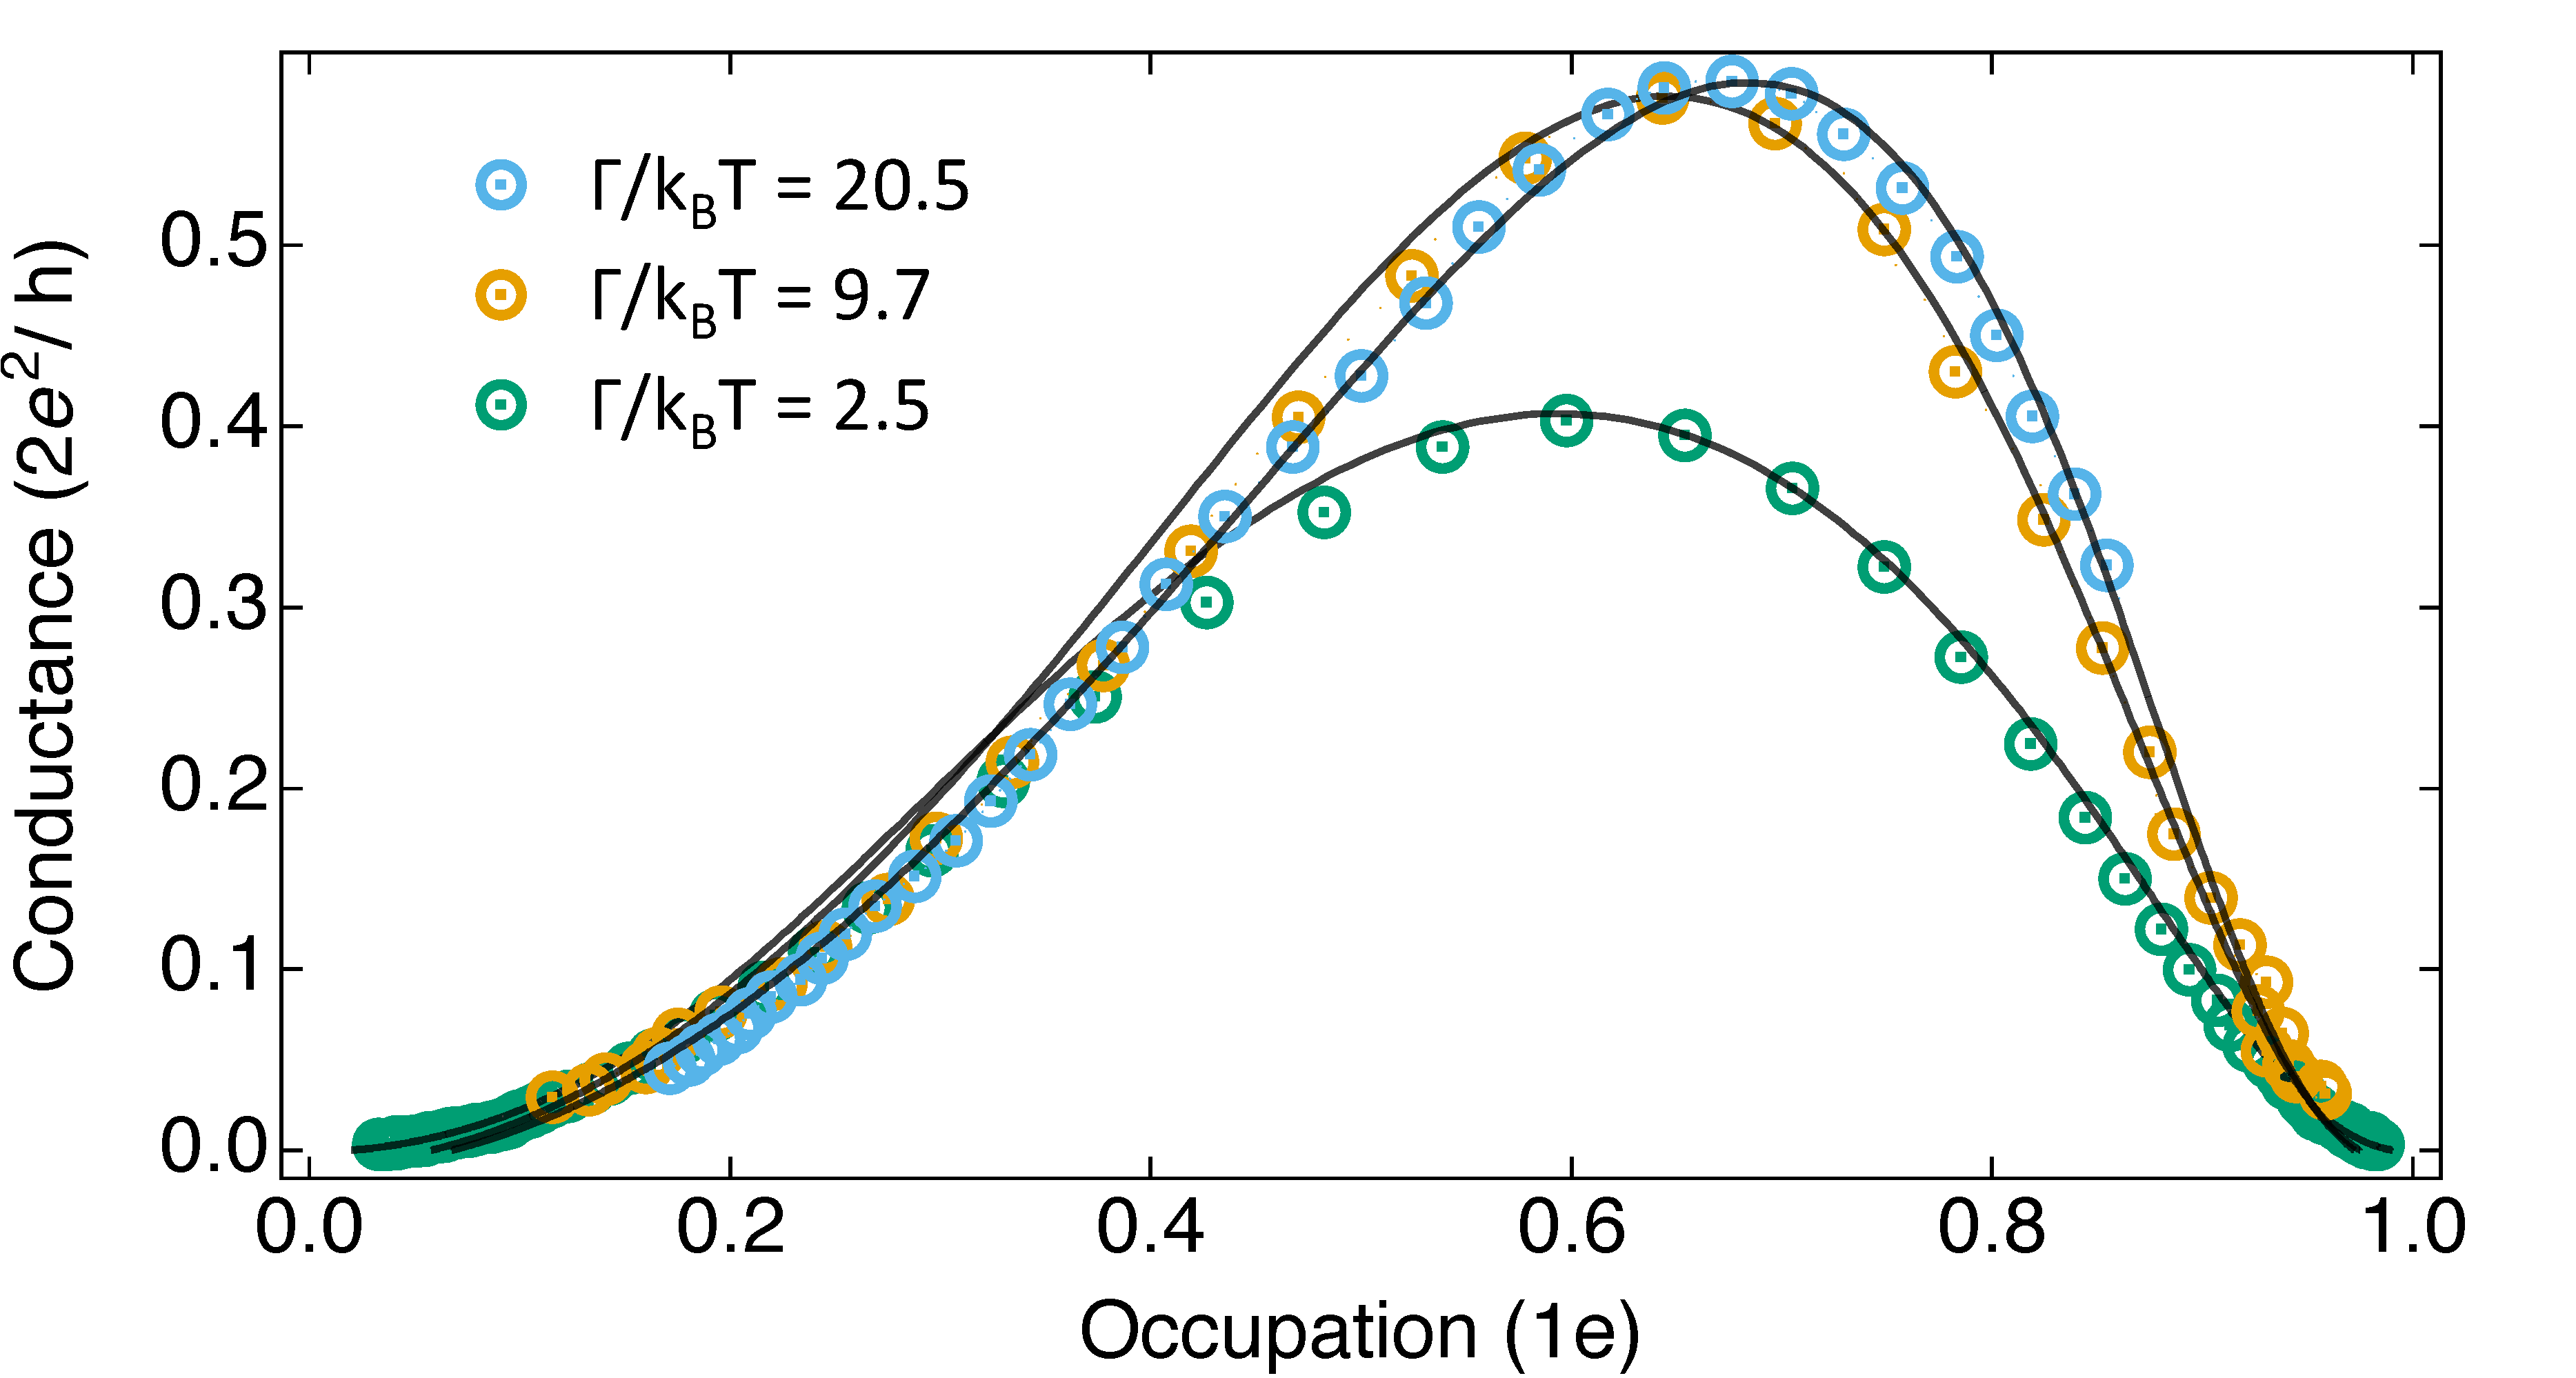
\includegraphics[width=0.85\textwidth]{figures/ch3/figure15.pdf}
 \caption[Conductance versus Occupation : Varying Coupling Strength]{\label{fig:ch3/cond_occ_couplingstrength} 
 % For some options that work with pdf\LaTeX, please see this discussion:
 % \url{http://tex.stackexchange.com/questions/11839}. 
 Conductance versus occupation in a weak (green) and strong (blue) coupling regime. Each trace is taken at \qty{20}{mK}. The coupling strength $\mathrm{\Gamma/k_BT}$ was determined from a global fit to multiple temperatures. The NRG (grey) conductance versus occupation corresponding to the determined $\mathrm{\Gamma/k_BT}$ is plotted on top of the data. Good agreement is found at each coupling strength.}
 \end{center}
\end{figure}


In Fig.~\ref{fig:ch3/cond_vs_occ_gf}\textbf{b}, the Kondo enhancement dependence on the system's temperature was confirmed. At high temperatures $\mathrm{T>T_K}$, there is no Kondo singlet, and so the conductance maximum is near $\mathrm{N} = 0.5$. But at low temperatures $\mathrm{T<T_K}$, a Kondo singlet is formed, and the conductance maximum shifts to higher occupation $\mathrm{N} > 0.5$. This displays the dependence of the Kondo temperature on the dot energy. The Kondo temperature rises as the dot energy gets close to the leads. However, the Kondo temperature also depends on the coupling strength between the quantum dot and leads Eq.~\ref{eq:kondo_temp}. As strongly coupled quantum dots have larger Kondo temperatures, the conductance maximum is expected to occur at higher occupation than in weakly coupled quantum dots. 



Figure~\ref{fig:ch3/cond_occ_couplingstrength} shows \qty{20}{mK} traces of conductance versus occupation at three different coupling strengths. $\mathrm{\Gamma/k_BT}$ is determined using the fitting routine described above to plot the corresponding NRG alongside the data. Expectedly, the more strongly coupled data shows a greater shift in the conductance maximum to higher occupation. Good agreement with NRG is observed at each coupling.






% \afterpage{\clearpage}
% \afterpage{}
% \FloatBarrier
\section{Kondo Effect with Varying Charge Sensor Current}

This new method of plotting conductance versus occupation not only requires a reliable determination of $\mathrm{\Gamma/k_BT}$ and lever arm from conductance data, but also clean charge transitions that can be converted into an occupation. The shape of the charge transition can vary depending on the choice of virtual gate and the charge sensor QPC setpoint. In the next section, different current setpoints of the charge sensor QPC are measured and the resulting conductance versus occupation is tested for agreement with NRG.


% \afterpage{\clearpage}
\subsection{Varying Charge Transition}


\begin{figure}[!bht]
 \begin{center}
%% includegraphics: comment the following if not using the graphicx package
 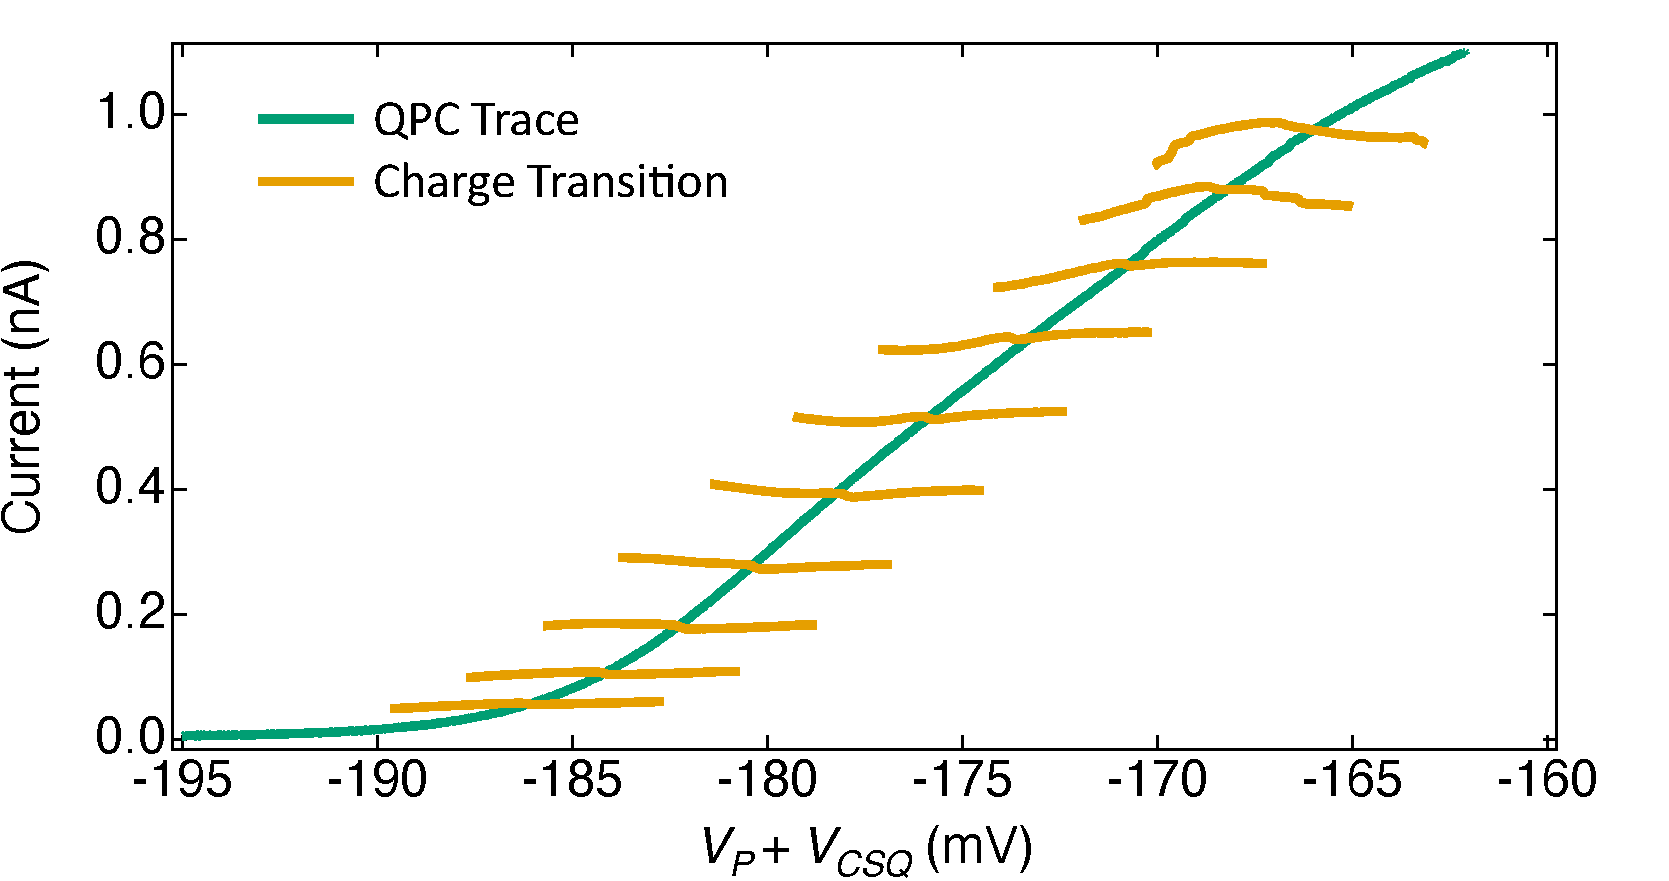
\includegraphics[width=0.85\textwidth]{figures/ch3/figure16.pdf}
 \caption[Varying Charge Sensor Current Setpoint]{\label{fig:ch3/cond_occ_ct_set-points} 
 % For some options that work with pdf\LaTeX, please see this discussion:
 % \url{http://tex.stackexchange.com/questions/11839}. 
 Current through the charge sensor (green) from pinch-off to the start of the first conductance plateau. Corresponding charge transition (yellow) at each current setpoint through the charge sensor. Note the x-axis is different between the underlying charge sensor trace and charge transitions. The charge transitions x-axis has been scaled the same amount for clarity. The charge transitions vary dramatically as the current through the charge sensor is changed. The left and right slopes curve upwards, downwards, in the same direction, or opposite each other.}
 \end{center}
\end{figure}
% \FloatBarrier


Figure~\ref{fig:ch3/cond_occ_ct_set-points} shows a charge sensor trace (green) and the resulting charge transition (yellow) at a range of current setpoints through the charge sensor. The current (y-axis) has not been scaled differently between the charge sensor trace and charge transitions. However, the sweep gate (x-axis) of the charge sensor and charge transitions are different. The charge transition sweep gate axis has been scaled for clarity in this plot. 



The shape of the charge transition varies significantly as the current setpoint through the charge sensor changes. Typically, the charge sensor is set to its steepest slope where the derivative is the largest. Here, the charge sensor is most sensitive as small changes in the potential result in large changes in the current. The resulting amplitude of the charge transition is greatest at the steepest slope. However, charge transitions can be measured at any current setpoint through the charge sensor. As long as the change in current through the charge sensor is linear with respect to the change in voltage. This can be achieved with a virtual gate, which keeps the current through the charge sensor constant. 



Yet, at each charge sensor current setpoint, the charge transition slopes vary differently on the unoccupied and occupied sides. Comparing the slopes on the unoccupied (left) side, at low currents, they point downwards, then point upwards with increasing current, and then point downwards again at the highest current setpoint. It is important to show that the conduction versus occupation agrees with NRG, irrespective of the current setpoint through the charge sensor. Otherwise, it may be possible to `pick' a current setpoint through the charges sensor that either shows or does not show agreement with NRG. This would render the method unreliable. 




\subsection{Conductance versus Occupation}



\begin{figure}[!hbt]
 \begin{center}
%% includegraphics: comment the following if not using the graphicx package
 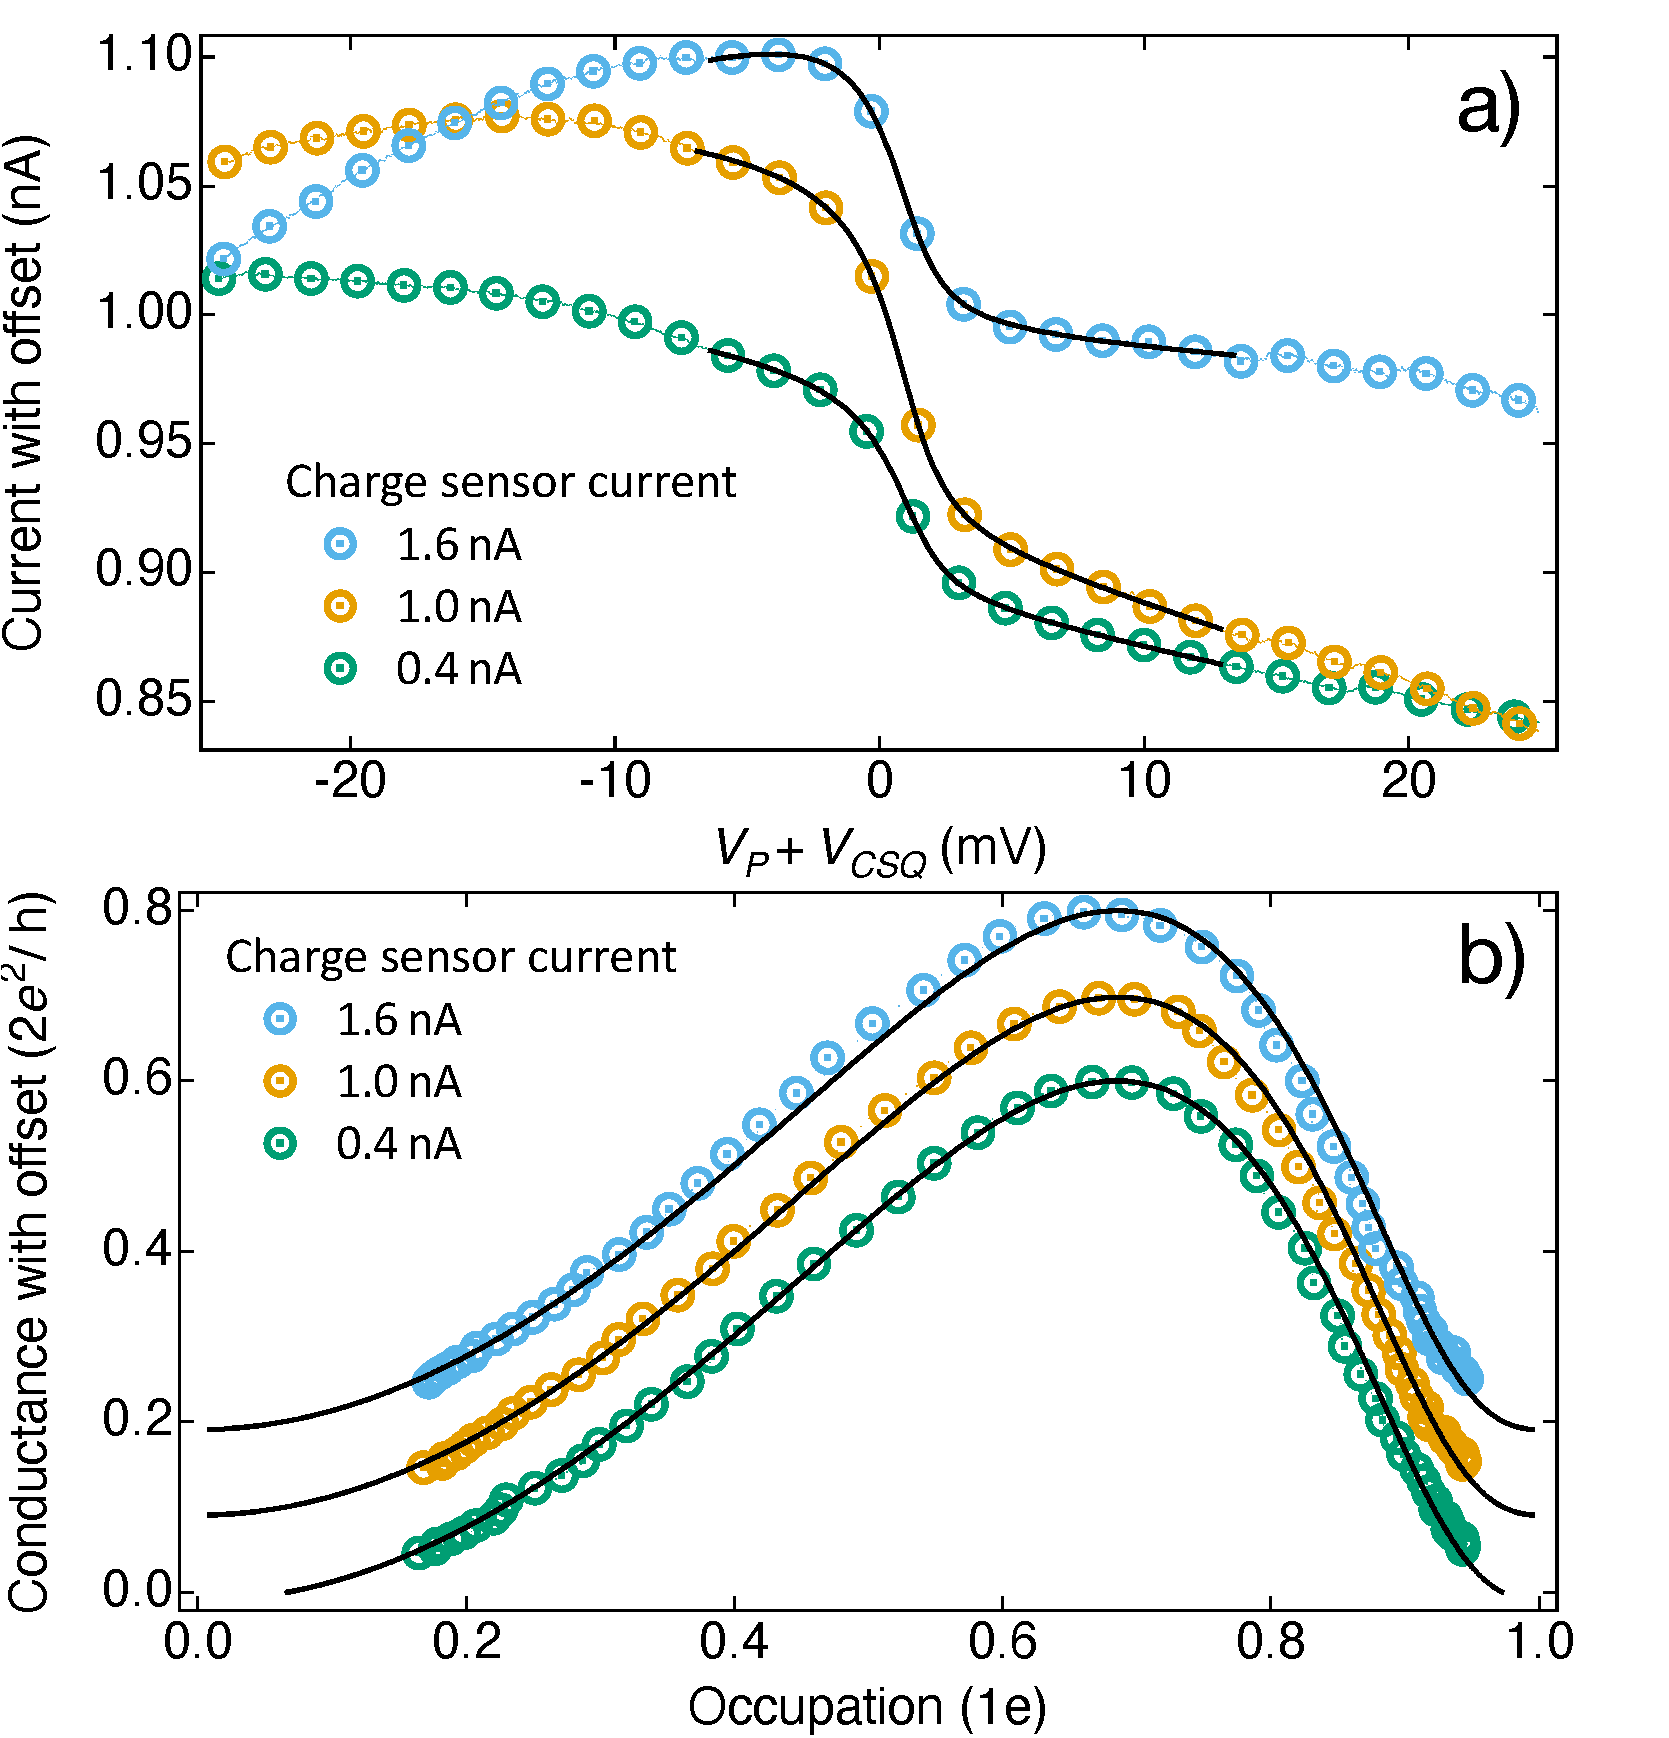
\includegraphics[width=0.85\textwidth]{figures/ch3/figure17.pdf}
 \caption[Conductance versus Occupation : Varying Charge Sensor Current]{\label{fig:ch3/cond_occ_QPC_vs_ct} 
 % For some options that work with pdf\LaTeX, please see this discussion:
 % \url{http://tex.stackexchange.com/questions/11839}. 
 (\textbf{a}) Charge transitions are measured with high (blue) and low (green) current through the charge sensor. For clarity, the transitions are offset in the current. The x-axis uses the same virtual gate for each charge transition. The slopes on either side of the charge transitions vary with the current through the charge sensor, suggesting the best virtual gate also changes. (\textbf{b}) Conductance versus occupation ($\mathrm{\Gamma/k_BT=21}$) at different current setpoints through the charge sensor. The traces are offset for clarity. Each trace is taken at \qty{20}{mK}. The coupling strength $\mathrm{\Gamma/k_BT}$ was determined from a global fit to conductance at multiple temperatures. The NRG (grey) conductance versus occupation, corresponding to the determined $\mathrm{\Gamma/k_BT}$, is plotted on top of the data. Good agreement is found at each current setpoint.}
 \end{center}
\end{figure}


Figure~\ref{fig:ch3/cond_occ_QPC_vs_ct}\textbf{a} shows charge transitions taken at \qty{20}{mK} for three different current setpoints through the charge sensor. For clarity, each charge transition has been offset in the current. The shape of the charge transition clearly depends on the current through the charge sensor. The unoccupied (left) side of the high current (blue) charge transition slopes down, whilst the low current (green) charge transition slopes upwards. This suggests that the optimal virtual gate to keep the charge sensor current constant also changes. At each current setpoint, conductance was simultaneously measured at a range of temperatures. A global fit to the conductance was used to determine $\mathrm{\Gamma/k_BT}$ and lever arm. Each charge transition was converted into an occupation, and the conductance versus occupation is plotted with a comparison to NRG (Fig.~\ref{fig:ch3/cond_occ_QPC_vs_ct}\textbf{b}). For clarity, the conductance versus occupation traces have each been offset by \qty{0.1}{2e^2/h}. Excellent agreement between data and NRG is found at each current setpoint. 


% \afterpage{\clearpage}
\section{Kondo Effect with Varying Coupling Symmetry}

All previous conductance data shown in this thesis was taken with symmetric coupling ($\mathrm{\Gamma_R = \Gamma_L}$). Previous measurements of the Kondo effect also tune the quantum dot to be symmetrically coupled with the source and drain leads. However, some experimental studies have investigated the Kondo effect with asymmetric coupling ($\mathrm{\Gamma_R \neq \Gamma_L}$)~\cite{kondo_asymmetric}. It was found that the characteristic zero bias peak between Coulomb peaks shifted to a nonzero bias. However, this effect would require a strong energy dependence of the tunnel barriers (i.e., $\mathrm{\Gamma = \Gamma(E)}$) in a NRG calculation, which is not assumed in our current NRG calculations.
Hence, a measurement of conductance with nonzero bias cannot be currently compared to NRG. 
Although we may not quantitatively corroborate these previous findings, exploring coupling symmetry is interesting as it effectively tests how the Kondo enhancement varies when a quantum dot is coupled to two leads (symmetric case) versus a single lead (asymmetric case). In practice, the limit of a single lead regime cannot be reached, as conductance will not be measured through the quantum dot.


% \afterpage{\clearpage}
\subsection{Symmetric to Asymmetric}


\begin{figure}[!hbt]
 \begin{center}
%% includegraphics: comment the following if not using the graphicx package
 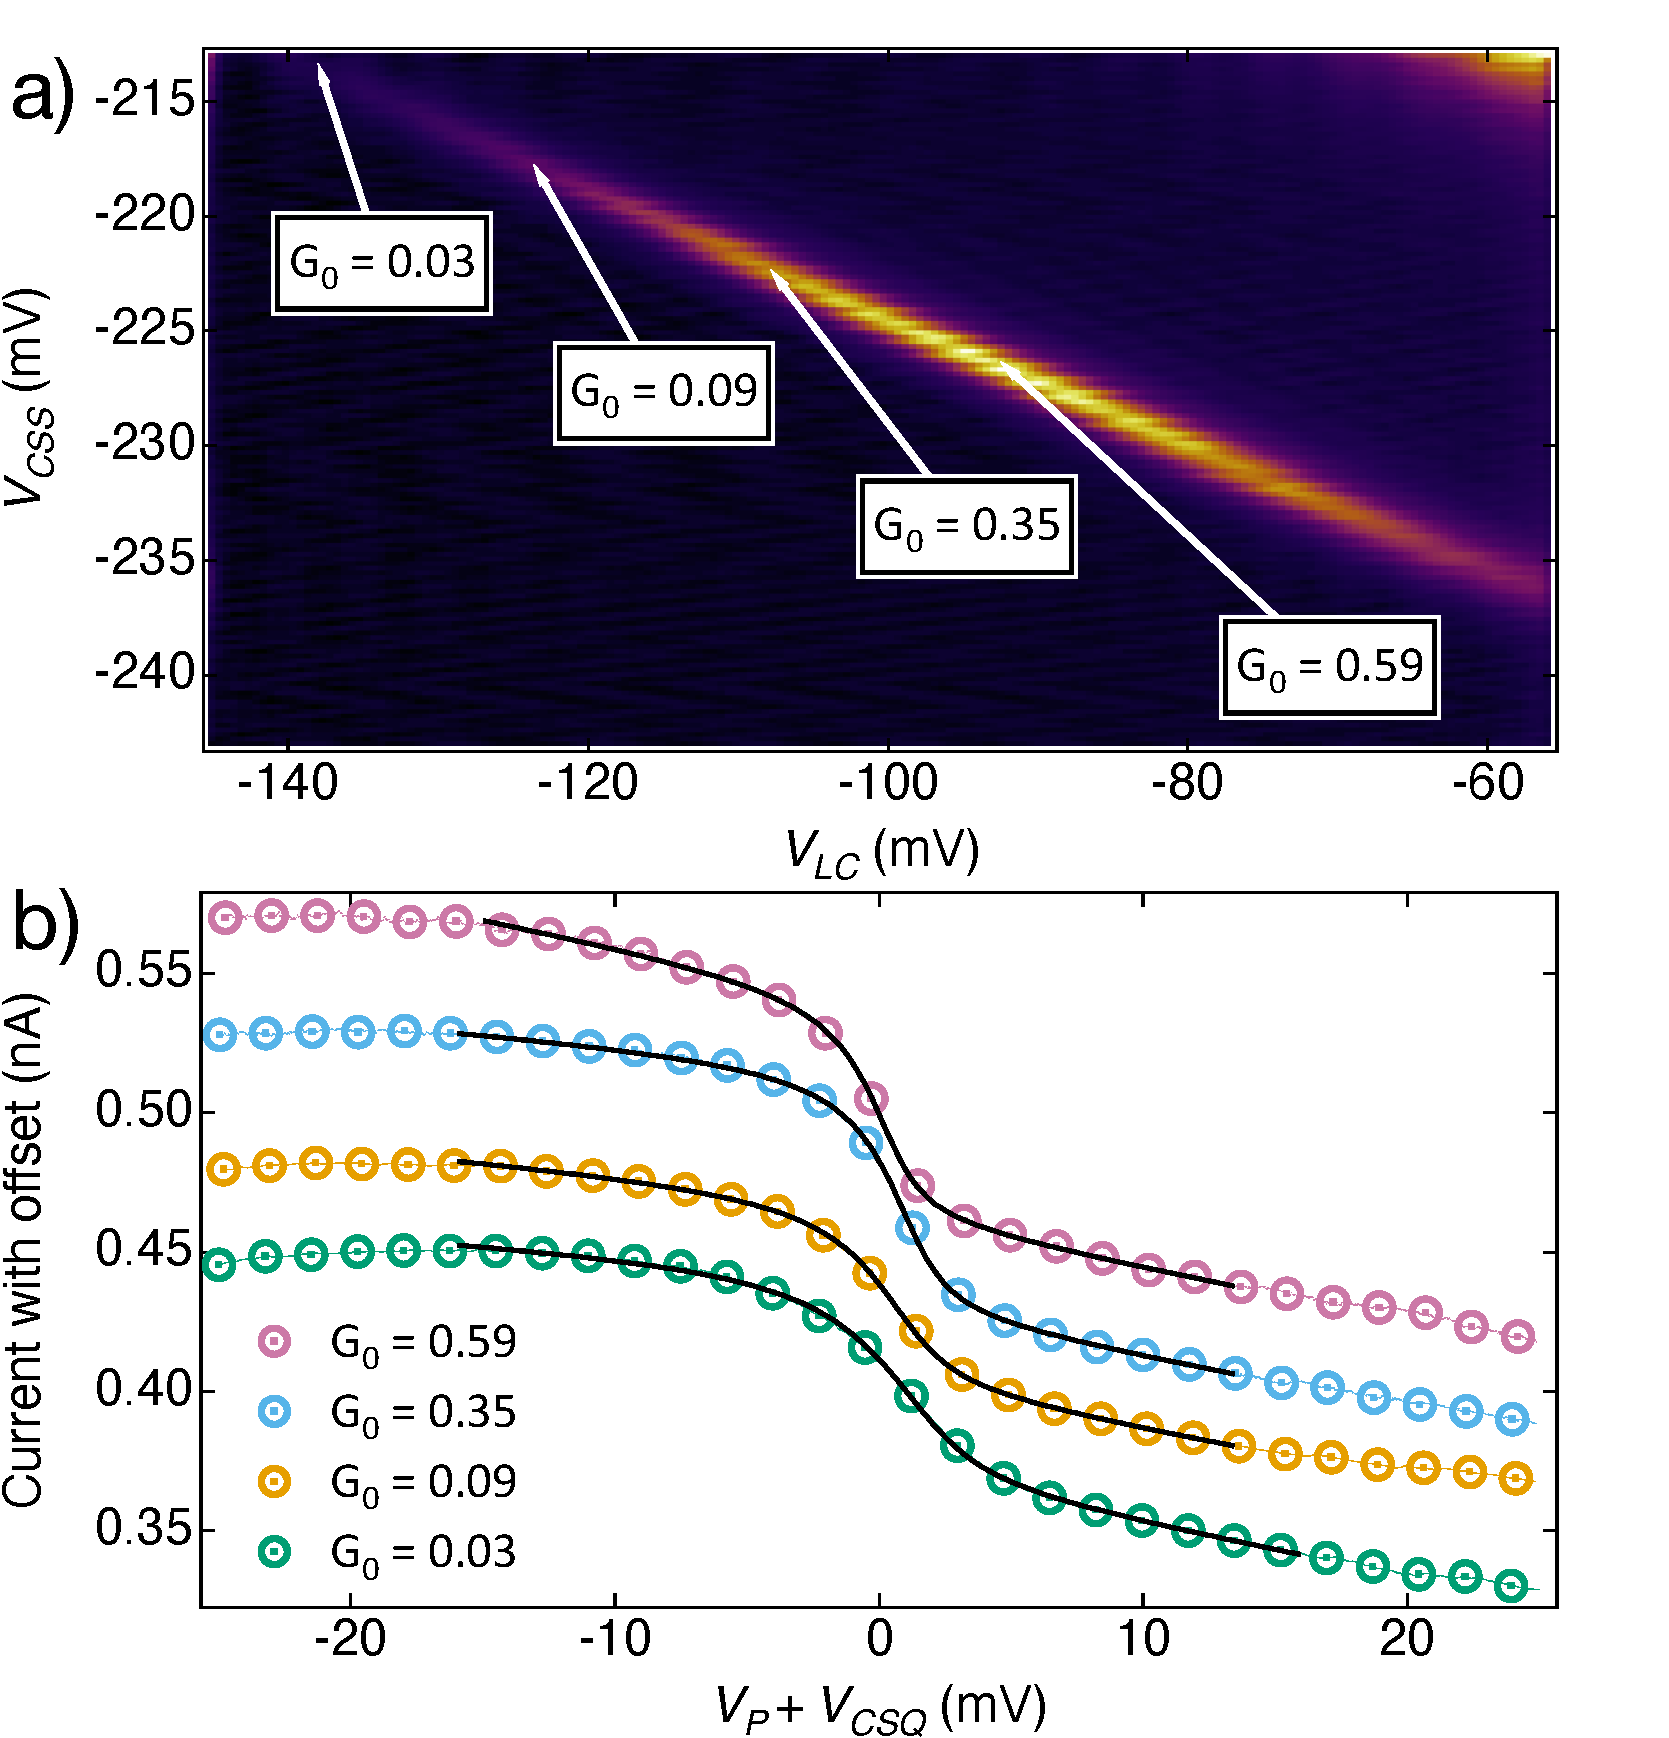
\includegraphics[width=0.85\textwidth]{figures/ch3/figure18.pdf}
 \caption[Symmetric to Asymmetric Coupling]{\label{fig:ch3/symmetry_picking} 
 % For some options that work with pdf\LaTeX, please see this discussion:
 % \url{http://tex.stackexchange.com/questions/11839}. 
 (\textbf{a}) 2D scan of conductance through the quantum dot varying the two coupling gates V\textsubscript{CSS}, and V\textsubscript{LC}. In the top left, the dot is more coupled to the right lead than the left as V\textsubscript{LC} is made more negative. In the middle of the scan (where the conductance is maximum), the coupling is symmetric $\mathrm{\Gamma_R} = \mathrm{\Gamma_L}$ (\textbf{b}) Charge transitions measured with different ratios of coupling between the two leads in the dot. $\mathrm{G_0} = 0.59$ is symmetric coupling (pink), $\mathrm{G_0} = 0.03$ is asymmetric coupling (green). For clarity, the transitions are offset in the current. But have been measured with roughly the same current setpoint through the charge sensor ($\sim\qty{0.4}{nA}$). The x-axis uses the same virtual gate for each charge transition. 
 % The charge transitions become more strongly coupled as asymmetric increases (pink-green)
 }
 \end{center}
\end{figure}


The width of a strongly coupled Coulomb peak is controlled by $\Gamma$. Where $\Gamma$ is the sum of the individual tunnelling rates, $\Gamma=\mathrm{\Gamma_L} + \mathrm{\Gamma_R}$. 
The conductance amplitude in both the weakly (Eq.~\ref{eq:cond_amp}) and strongly (Eq.~\ref{eq:cond_amp_strong}) coupled regimes depend on $\Gamma$. Hence, the conductance amplitude can be used as a marker of how asymmetrically coupled the quantum dot is to the leads. 


To vary the coupling symmetry in a quantum dot, a 2D scan measuring the conductance with gates that control a separate coupling on each axis is used. In Fig.~\ref{fig:ch3/symmetry_picking}\textbf{a}, V\textsubscript{CSS} (y-axis) mainly controls $\mathrm{\Gamma_R}$, and V\textsubscript{LC} (x-axis) mainly controls $\mathrm{\Gamma_L}$. Four points are picked from symmetric coupling (middle of scan) to asymmetric coupling (top left of scan), where the dot becomes more strongly coupled to the right lead. 
% The ratio $\mathrm{\Gamma_L}/\mathrm{\Gamma_R}$ was only calculated after the conductance global fit to NRG, which determined $\Gamma$. 




Charge transitions were simultaneously measured so that conductance versus occupation could be compared with the corresponding NRG. 
Charge transitions for each coupling setpoint were measured with $\sim\qty{0.4}{nA}$ through the charge sensor (Fig.~\ref{fig:ch3/symmetry_picking}\textbf{b}). 
Each charge transition did not have charge jumps near the transition and was deemed a reliable measure of the occupation. Interestingly, the asymmetrically coupled transition (green) is more broadened than the symmetrically coupled transition (pink). $\mathrm{\Gamma/k_BT}$ determined from the global fit to conductance varied from 20.5 for symmetric coupling to 26.0 for asymmetric coupling. However, a global fit to the charge transitions finds 19.6 for symmetric coupling and 45.0 for asymmetric coupling (Table~\ref{tab:sym_coupling_gf}). 
% \newcolumntype{P}[1]{>{\centering\arraybackslash}p{#1}}

\begin{table}[!hbt] 
\centering
\begin{tabular}{|c|c|c|}
% \begin{tabular}{|c{2.0cm}|c{4.0cm}|c{4.0cm}|}
\hline
\multicolumn{1}{|c|}{} & \multicolumn{2}{c|}{$\mathrm{\Gamma/k_BT}$ from Global Fit}\\
\hline
 $\mathrm{G_0}\,(\qty{}{2e^2/h})$ & Conductance Fit & Charge Transition Fit \\
\hline
0.59 & 20.5 & 19.6 \\
0.35 & 22.0 & 21.6 \\
0.09 & 24.4 & 30.9\\
0.03 & 26.0 & 45.0\\
\hline
\end{tabular}
 \caption[$\mathrm{\Gamma/k_BT}$ From Conductance and Charge Transition Global Fits]{\label{tab:sym_coupling_gf} $\mathrm{\Gamma/k_BT}$ determined from a global fit to conductance and separately a global fit to charge transitions at different ratios of coupling symmetry. At symmetric coupling ($\mathrm{G_0}=0.59$), the determined $\mathrm{\Gamma/k_BT}$ from conductance and charge transitions are similar. However, at asymmetric coupling ($\mathrm{G_0}=0.03$), the $\mathrm{\Gamma/k_BT}$ from a global fit to charge transitions is much greater than from a global fit to conductance.}
\end{table}


% \afterpage{\clearpage}
\subsection{Conductance versus Occupation}



\begin{figure}[!bht]
 \begin{center}
%% includegraphics: comment the following if not using the graphicx package
 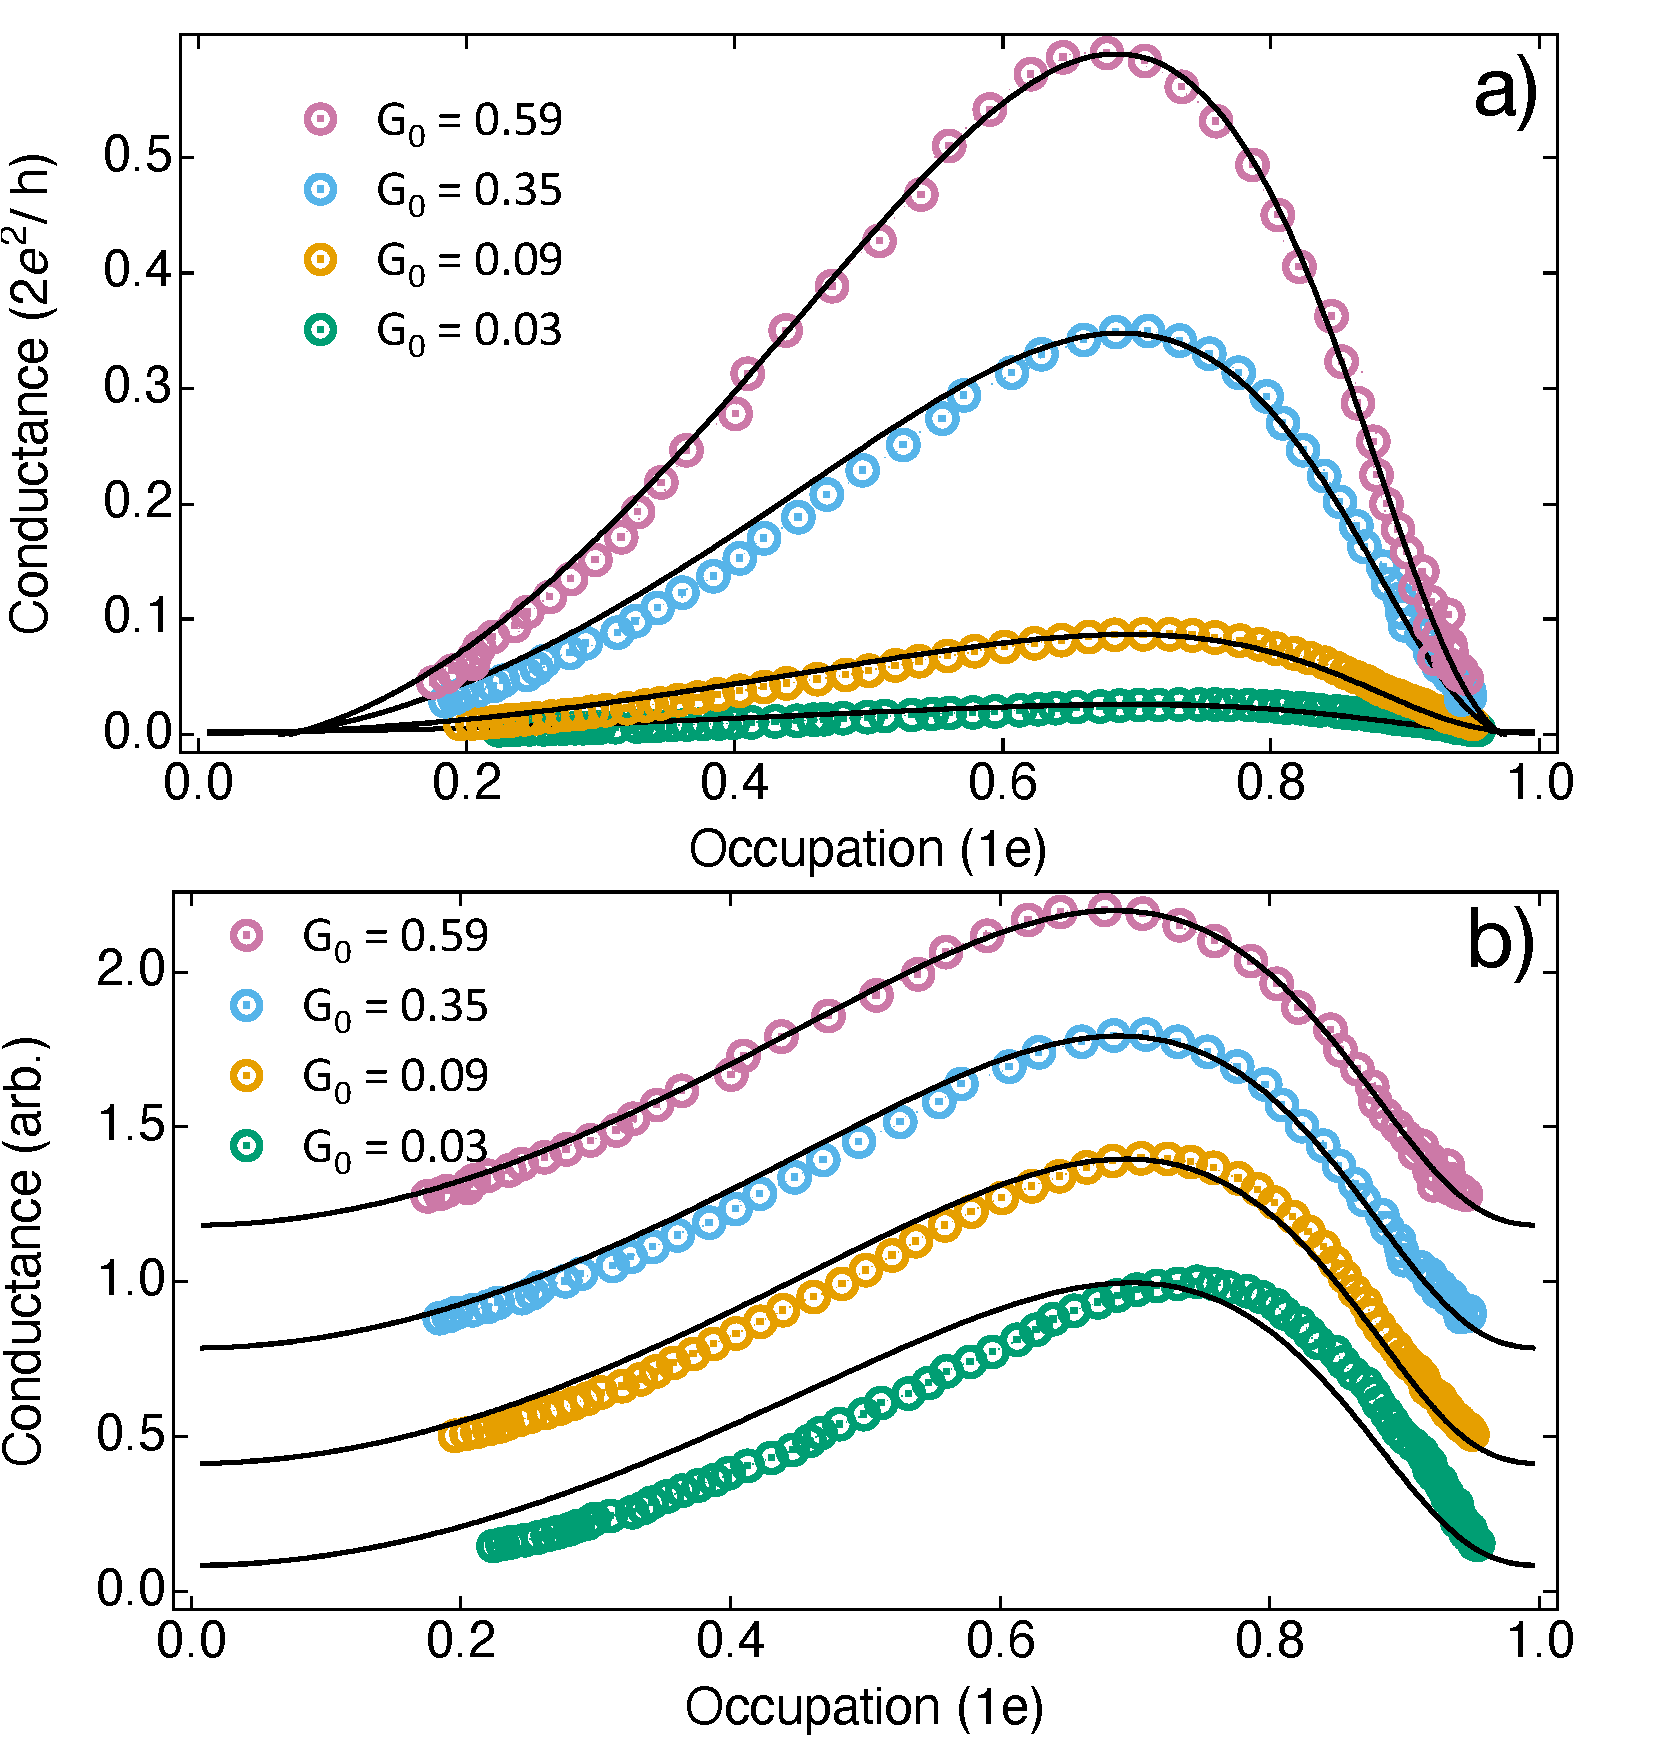
\includegraphics[width=0.85\textwidth]{figures/ch3/figure19.pdf}
 \caption[Conductance versus Occupation : Varying coupling symmetry]{\label{fig:ch3/cond_occ_assymetry} 
 % For some options that work with pdf\LaTeX, please see this discussion:
 % \url{http://tex.stackexchange.com/questions/11839}. 
 (\textbf{a}) Conductance versus occupation ($\mathrm{\Gamma/k_BT=21}$) with different ratios of coupling symmetry between the two leads of the dot. As the asymmetry is increased, the conductance decreases.
 (\textbf{b}) Same data as in (\textbf{a}), except the traces are offset and scaled for clarity. Symmetric coupling agrees well with NRG calculations. However, the asymmetrically coupled data is shifted to the right of the predicted NRG. This suggests that $\mathrm{\Gamma/k_BT}$ extracted from the global fit to conductance is lower than expected.}
 \end{center}
\end{figure}


Figure~\ref{fig:ch3/cond_occ_assymetry}\textbf{a} shows conductance versus occupation taken at \qty{20}{mK} at the four different ratios of coupling symmetry found in Fig.~\ref{fig:ch3/symmetry_picking}\textbf{a}. There is good agreement with NRG in the symmetric coupling (pink). However, as the coupling becomes more asymmetric, the conductance amplitude decreases (Eq.~\ref{eq:cond_amp_strong}), and agreement with NRG is difficult to determine. Hence, for clarity, Fig.~\ref{fig:ch3/cond_occ_assymetry}\textbf{b} shows the same data with an added scaled and offset. The corresponding NRG was also scaled and offset the same as the data. A disagreement between asymmetric coupling (green) data and NRG becomes much clearer. When asymmetrically coupled, the conductance maximum of the data is shifted to the right of the NRG. This suggests the $\mathrm{\Gamma/k_BT}$ determined from the global fit to conductance is lower than expected. 



This discrepancy with NRG is surprising as conversations with our theorist collaborators suggest that NRG only depends on the overall $\Gamma$, and not the ratio between $\Gamma_\mathrm{L}$ and $\Gamma_\mathrm{R}$.
Perhaps some mechanism could be altering the shape or location of the conductance. 
Previous experiments have used a charge sensor as a noise source to de-phase the Kondo singlet~\cite{kondo_controlled_dephasing}. In these studies, the bias across the charge sensor was \qty{1200}{\micro V}, twelve times the bias that is used for the charge sensor in this thesis (\qty{100}{\micro V}) and the suppression of the measured conductance was $\sim6\%$. 
A more recent theoretical study found that for weak coupling between the charge sensor and quantum dot, the spectral weight of the Kondo resonance is reduced, leading to a suppression of the conductance. However, the width of the resonance is not affected, suggesting the absence of dephasing~\cite{peculiar_dephasing_of_kondo}. Although this de-phasing mechanism could result in the conductance maximum being shifted to a lower occupation, it would not explain a shift to a higher occupation or the dependence on symmetric coupling.


Instead of a change in the shape or location of the conductance, it is possible the charge transition behaves differently between coupling symmetries. 
Numerous studies have investigated the tunnelling rates onto and off the quantum dot~\cite{MacLean2007,Ihn2009,Kng2012}, with differing barrier symmetries~\cite{Rogge2005,Gustavsson2006}. However, these studies required the source-drain bias to be larger than the temperature broadening, so the results cannot be extrapolated to our regime of zero bias. 

An early study on the shape of the charge transition with symmetric coupling found that in the absence of a magnetic field, charge transitions are unaffected by the onset of Kondo correlations~\cite{Sprinzak2002}. It was argued that the conductance enhancement between Coulomb peaks results from a larger number of electrons traversing the quantum dot, each dwelling there for a shorter time. However, coupling symmetry was not explored in this experiment. 


 The most promising insight comes from very recent theoretical studies of the differential conductance through a quantum dot and its dependence on asymmetry in the tunnel barriers and source-drain bias~\cite{Tsutsumi2021,kondo_nrg_asymmetric}. 
 It was found that higher-order corrections to the differential conductance include non-linear terms that depend strongly on the tunnelling and bias asymmetries. As an example, for $\Gamma_\mathrm{L}>\Gamma_\mathrm{R}$, the number of electrons entering the quantum dot from the left side becomes larger than the number of electrons leaving the right side. Therefore, the number of electrons in the dot increases and the repulsive interaction increases $\tilde{\epsilon}_0$. In contrast, $\tilde{\epsilon}_0$ would decrease for $\Gamma_\mathrm{L}<\Gamma_\mathrm{R}$. This modification to $\tilde{\epsilon}_0$ can result in increased or decreased conductance. 

It should be noted that the exploration of symmetric coupling in this thesis only came from two overnight measurements in a single cooldown and a second cooldown is required to verify the findings. Additionally, a subsequent cooldown would allow for a more focused exploration of tunnel coupling and bias symmetry. 
 




% \clearpage
% \section{Discussion}




\chapter{Conclusion}\label{cha:conclusion}


\epigraph{``Nothing in life is to be feared, it is only to be understood. Now is the time to understand more, so that we may fear less.''}{Marie Curie}

\noindent In conclusion, a method has been demonstrated to study the conductance enhancement from the Kondo effect, in a more weakly coupled regime than has been previously explored. 
Previous studies have predominantly focused on very strong coupling, where the Kondo temperature exceeds the system temperature, even between Coulomb peaks.
Weaker coupling reveals a markedly different behaviour: the Kondo temperature is significantly lower than the system temperature between Coulomb peaks, resulting in a lack of conductance enhancement.
Nonetheless, as the dot energy approaches the Fermi energy of the source and drain leads, the Kondo temperature increases exponentially. 
Consequently, even under relatively weak coupling, a small conductance enhancement persists on the shoulder of odd occupation Coulomb peaks.




To reliably measure this small conductance enhancement, a new method is required to disentangle the effects of charge motion, entropy, and Kondo enhancement on the shape and location of the conductance. 
The approach relies on two key components. 
The first component is a simultaneous measurement of a conductance and charge transition. The charge transition is then used to determine the occupation of the quantum dot. This occupation is used as a reference to remove the effects of charge motion and entropy. When conductance is plotted against the occupation, a shift in the maximum conduction to higher occupation suggests Kondo enhancement. 
The second component is measuring conductance at a range of temperatures that cross into the temperature broadened regime, $\mathrm{\Gamma/k_BT} \lesssim 1$. A global fit to NRG, including each temperature setpoint is used to reliably determine $\mathrm{\Gamma/k_BT}$ and lever arm. The determined $\mathrm{\Gamma/k_BT}$ is then used to compare data with NRG to test agreement. 

Agreement between data and corresponding NRG is seen at coupling strengths $\mathrm{\Gamma/k_BT} = 20.5$, $\mathrm{\Gamma/k_BT} = 9.7$ and $\mathrm{\Gamma/k_BT} = 2.5$. The most strongly coupled data ($\mathrm{\Gamma/k_BT} = 20.5$) shows the greatest shift in conductance maximum towards higher occupation. 
A reliable measurement of the charge transition is critical to determine the occupation of the quantum dot. 
Hence, various current setpoints through the charge sensor were tested to ensure independence from the charge sensor's settings.
Despite differences in the underlying charge transition shape across current setpoints, agreement with NRG was consistently observed.
To investigate the influence of coupling symmetry on Kondo enhancement, four ratios of coupling symmetry were measured.
Good agreement with NRG was found with symmetric coupling. 
However, a shift towards greater occupation than predicted by NRG was observed as coupling symmetry became more asymmetric.
This discrepancy suggests a difference between the $\mathrm{\Gamma/k_BT}$ value determined from the global fits to conductance and that which best matches the corresponding charge transitions. 
To validate this observation, separate global fits to conductance and charge transitions were performed. Under symmetric coupling, the determined $\mathrm{\Gamma/k_BT}$ values agree. However, as asymmetry increases, the $\mathrm{\Gamma/k_BT}$ obtained from the charge transitions is significantly larger than that from the conductance fits.
The discrepancy with NRG is surprising as conversations with our theorist collaborators suggest that NRG only depends on the overall $\Gamma$, and not the ratio between $\Gamma_\mathrm{L}$ and $\Gamma_\mathrm{R}$.

To my knowledge, only one other experiment has investigated the effects of coupling symmetry on the Kondo effect~\cite{kondo_asymmetric}. 
It was found that the characteristic zero bias peak between Coulomb peaks shifted to a nonzero bias. However, this effect would require a strong energy dependence of the tunnel barriers (i.e., $\mathrm{\Gamma = \Gamma(E)}$) in a NRG calculation, which is not assumed in our current NRG calculations.

An interesting insight into our observed discrepancy comes from very recent theoretical studies of the differential conductance through a quantum dot and its dependence on asymmetry in the tunnel barriers and source-drain bias~\cite{Tsutsumi2021,kondo_nrg_asymmetric}. It was found that higher-order corrections to the differential conductance include non-linear terms that depend strongly on the tunnelling and bias asymmetries. However, corrections to the differential conductance in this paper require an applied bias across the quantum dot. As the measurements in this thesis were conducted in an effective zero bias limit (\qty{1}{\micro V} bias), it is unclear whether the discrepancy can be explained by this theory. A further cooldown would allow for a more focused exploration of tunnel coupling symmetry, bias symmetry and total applied bias. If our data qualitatively matches these recent theory predictions, a new calculation of our NRG, including bias and tunnel coupling symmetry may be required. 
 

Finally, a recent study observed the change in entropy as an electron entered a quantum dot (coupled to a single lead) with similar coupling strengths as those in this thesis~\cite{child_strong}. 
A suppression of the entropy was reported, however, the expected shift in the entropy onset was not seen in the data. 
In contrast, the measurements on asymmetric coupling in this thesis found the conductance maximum shifts towards greater occupation than predicted by NRG.
Perhaps a device capable of measuring entropy and conductance with two leads holds promise for illuminating this discrepancy.






% \section{Programs}
% Here we give an example of a new float as defined using the
% \texttt{float} package.  In the preamble we have used the commands
% \begin{verbatim}
% \floatstyle{ruled}
% \newfloat{Program}{htbp}{lop}[chapter]
% \end{verbatim}
% This creates a ``Program'' environment that may be used for program
% fragments.  A sample \texttt{python} program is shown in
% Program~\ref{prog:fib}.  (Note that Python places a fairly restrictive
% limit on recursion so trying to call this with a large $n$ before
% building up the cache is likely to fail unless you increase the
% recursion depth.)
% \begin{Program}
%   \caption{\label{prog:fib} Python program that computes the $n^{\rm
%       th}$ Fibonacci number using memoization.}
% \begin{verbatim}
% def fib(n,_cache={}):
%     if n < 2:
%         return 1
%     if n in _cache:
%         return _cache[n]
%     else:
%         result = fib(n-1)+fib(n-2)
%         _cache[n] = result
%         return result
% \end{verbatim}
% \end{Program}
% Instead of using a \texttt{verbatim} environment for your program
% chunks, you might like to \texttt{include} them within an
% \texttt{alltt} envrironment by including the \verb|\usepackage{alltt}|
% package (see page 187 of the \LaTeX{} book).  Another useful package
% is the \verb|\usepackage{listings}| which can pretty-print many
% different types of source code.

% Force a new page
\newpage

%% Here we provide a short optional argument to \chapter[]{}.  This
%% optional argument will appear in the table of contents.  For long
%% titles, one should use this to give a single-line entry to the
%% table of contents.
% \chapter[Another Chapter\ldots]{Another Chapter with a Very Long
%   Chapter-name that will Probably Cause Problems}
% \label{cha:apple_ref}

% This chapter name is very long and does not display properly in the
% running headers or in the table of contents.  To deal with this, we
% provide a shorter version of the title as the optional argument to the
% \verb|\chapter[]{}| command.

% For example, this chapter's title and associated table of contents heading and
% running header was created with\\
% \verb|\chapter[Another Chapter\ldots]{Another Chapter with a Very Long|\\
% \verb|Chapter-name that will Probably Cause Problems}|.

% Note that, according to the thesis regulations, the heading included
% in the table of contents must be a truncation of the actual heading.




% \section*{An Unnumbered Section That is Not Included in the Table of
%   Contents}

\afterpage{\clearpage}

%% This file is setup to use a bibtex file sample.bib and uses the
%% plain style.  Other styles may be used depending on the conventions
%% of your field of study.
%%
%%% Note: the bibliography must come before the appendices.
% \bibliographystyle{plain}
% \bibliography{bibliography}

\printbibliography

%% Use this to reset the appendix counter.  Note that the FoGS
%% requires that the word ``Appendices'' appear in the table of
%% contents either before each appendix lable or as a division
%% denoting the start of the appendices.  We take the latter option
%% here.  This is ensured by making the \texttt{appendicestoc} option
%% a default option to the UBC thesis class.

%%% If you only have one appendix, please uncomment the following line.
% \renewcommand{\appendicesname}{Appendix}
\appendix
\chapter{First Appendix}\label{cha:appendix1}


During my Master's I was trained by Tim Child on the necessary fabrication steps to add inner and outer gates forming the quantum devices. Once fully qualified, I fabricated some devices on my own. There are a number of required steps to turn the GaAs/AlGaAs heterostructures received from Michael Manfra's group into the chip that we can add the inner and outer gates. It should also be noted that I made no contribution to the nano fabrication recipes and simply followed the procedure developed by previous student. The following summary is largely adapted from Owen Sheekey's thesis, a past student from the Quantum Devices Group. 

\section{Summary}
The GaAs substrates are grown by Michael Manfra’s group at Purdue University. There are two key features to devices built on GaAs/AlGaAs 2DEGs – ohmic contact to the 2DEG and gating structures. In overview, devices used for this project use a thin film of $\mathrm{Al_2O_3}$ to electrically isolate top gates fabricated from Au/Ti. Ohmic contacts are made using annealed Ni/Au/Ge.

The general process of preparation of a sample goes as follows:

\begin{enumerate}
\item Gallium removal from back of wafers.
\item Ohmic contact: Lithography, evaporation, annealing.
\item Mesa etching: Lithography, $\mathrm{H_2SO_4}$ etching.
\item Atomic layer deposition: $\mathrm{Al_2O_3}$.
\item Gating (2 steps): Lithography, evaporation.
\item Wire bonding
\end{enumerate}

\section{Recipes}

\subsection{Gallium removal}
This is a recipe developed by Dr. Silvia Luescher Folk.


\begin{enumerate}
\item Cleave a full wafer into a quarter or half wafer. Blow off any dust bunnies from the surface before starting.
\item Spin a layer of AZ1518 resists at $4000 \,\mathrm{RPM}$ for $40\,\mathrm{s}$.
\item Bake the resist for $2\,\mathrm{minutes}$ at $100^\circ$C.
\item Put a clean wipe on a hotplate and set to $50^\circ$C. Put wafer face down (gallium side up) onto the clean wipe.
\item Wipe off gallium with q tips. Keep wiping until it is all gone.
\item Spin and bake another layer of AZ1518 ($4000 \,\mathrm{RPM}$ $40\,\mathrm{s}$ and bake $100^\circ$C $2\,\mathrm{minutes}$).
\item Etch $2 \,\mathrm{minutes}$ in full strength HCl. Quench etch by transferring to DI water.
\item Rinse well in DI water. Blow dry.
\item Squirt down with Acetone to strip resist from the surface and immediately rinse with IPA.
\item Soak 3~minutes each in Toluene, Acetone, and IPA. Rinse with IPA and blow dry between each solvent. Spray down with DI water and blow dry.
\end{enumerate}

\subsection{Mesa etch}
\begin{enumerate}
\item Solvent clean – Acetone, IPA. Rinse in DI, blow dry with $\mathrm{N_2}$.
\item Prebake chip for \qty{60}{s} at $110^\circ$C.
\item AZ5214-E  in positive mode, ramp up 500 RPM  for \qty{2}{s}, spin at 4444 RPM for \qty{40}{s} with \qty{60}{s} softbake at $100^\circ$C.
\item Photo lithography in MLA150 Heidelberg (Maskless Aligner) : Expose \qty{90}{mJ/cm^2}, defocus -1 
\item Develop in MIF 300, $50\,\mathrm{s}$ stop develop in DI.
\item Hardbake for \qty{60}{s} at $120^\circ$C.
\item O2 plasma etch in Plasma etch PE 50, 60s.
\item Etch in $30\,\mathrm{mL}$ diluted Sulfuric acid (700 Water:3 $\mathrm{H_2S0_4}$) + $2 \,\mathrm{mL}$ $\mathrm{H_2O_2}$ at $18^\circ$C for \qty{50}{s}
\item Stop etch in DI water. Remaining resist can be removed with Acetone, IPA and DI.
\end{enumerate}




\subsection{Ohmic contact}

\subsubsection{Lithography and evaporation}


At the end of my Master's there was a sizeable effort to develop low resistance ohmics contacts by Vahid Mohaved and Dr. Silvia Luescher Folk. Here is the most up to date recipe. 


\begin{enumerate}
\item Solvent clean – Acetone, IPA, Ultrasound. Rinse in DI, blow dry with $\mathrm{N_2}$.
\item Dehydration bake chip for $1 \,\mathrm{minutes}$ at $110^\circ$C.
\item AZ5214-E  in image reversal mode, ramp up 500 RPM  for \qty{2}{s}, spin at 4444 RPM for \qty{50}{s} with \qty{60}{s} softbake at $90^\circ$C.
\item Photo lithography in MLA150 Heidelberg (Maskless Aligner) : Expose \qty{40}{mJ/cm^2}, defocus +1 
\item IR bake for \qty{30}{s} at $110^\circ$C.
\item Photo lithography in MLA150 Heidelberg : Flood exposure \qty{222}{mJ/cm^2}, defocus +1 
\item Develop in AZ300 MIF , $40\,\mathrm{s}$ stop develop in DI.
\item Hardbake for \qty{60}{s} at $110^\circ$C.
\item $\mathrm{O^2}$ plasma etch in Plasma etch PE 50, $15\,\mathrm{s}$.
\item Dip in $37\%$ HCI for \qty{20}{s}. Rinse with DI for \qty{120}{s}

\item Evaporate the following:

\begin{table}[H]     
\centering
  \begin{tabular}{|p{2.0cm}|p{2.0cm}|p{2.0cm}|}
    \hline
    Metal & Thickness & Rate\\
    \hline
    Ni & $7\,\mathrm{nm}$ & $1.0\,\mathrm{\dot{A}s^{-1}}$\\
    Ge & $80\,\mathrm{nm}$ & $1.3\,\mathrm{\dot{A}s^{-1}}$\\
    Au & $160\,\mathrm{nm}$ & $2.0\,\mathrm{\dot{A}s^{-1}}$\\
    Ni & $36\,\mathrm{nm}$ & $1.6\,\mathrm{\dot{A}s^{-1}}$\\
    Au & $80\,\mathrm{nm}$ & $1.7\,\mathrm{\dot{A}s^{-1}}$\\
    \hline
  \end{tabular}
\label{tab:ohmic_evaporation}
\end{table}
\item Liftoff in Acetone at $70^\circ$C.
\item Rinse in Acetone, IPA and blowdry with $\mathrm{N_2}$.
\end{enumerate}



\subsubsection{Annealing}
The following process was followed on the rapid thermal annealer made “in house” for annealing GaAs and other substrates. The basic idea is to use a bulb in a near vacuum (with some amount of forming gas – $\mathrm{H_2}$ + $\mathrm{N_2}$) to heat the sample to a high temperature for a limited amount of time. The metal film melts and diffuses through the GaAs substrate to make contact with the 2DEG, usually $30-200\,\mathrm{nm}$ below the surface.

\begin{enumerate}
\item Pump down should reach lower limit, $0.133\,\mathrm{mbar}$.
\item Set regulator to $2.5\,\mathrm{psi}$ (forming gas).
\item Open Swagelock valve until pressure reads $10\,\mathrm{mbar}$.
\item Close speedivalve until pressure reads $200\,\mathrm{mbar}$.
\item Turn on bulb to roughly $34\,\%$, it takes about $5-10\,\mathrm{minutes}$
\item Wait at $350^\circ$C for $2\,\mathrm{minutes}$
\item Go to $450^\circ$C as fast as you can, hold it there for $40\,\mathrm{s}$.
\item Cool below $300^\circ$C fast by opening the speedivalve on the pump line all the way, and opening the gas flow.
\item Cool to $50^\circ$C, then vent and let cool to room temperature.
\end{enumerate}


\subsection{Gating}
% \label{appendix:fab_gates}

Gating is the process of adding metal to the top of the GaAs/AlGaAs heterostructure which are used to form and control the potential landscape in the 2DEG below. The overall recipe of gating has not needed to be varied during my fabrication time. However, if long periods have passed between fabrication (few months) it is necessary to test an array of exposure doses for the E beam step as this parameter can vary over long periods of time and system re starts.





\subsubsection{Inner gates}

\begin{enumerate}
\item Solvent clean - Acetone, IPA. Rinse in DI, blow dry with $\mathrm{N_2}$.
\item Prebake chip for $3\,\mathrm{minutes}$ at $180^\circ$C.
\item Spin PMMA A2 495K at $5555\,\mathrm{RPM}$ for $50\,\mathrm{s}$  with $3\,\mathrm{minutes}$ bake at $180^\circ$C
\item Spin PMMA A1 950K at $3333\,\mathrm{RPM}$ for $50\,\mathrm{s}$  with $5\,\mathrm{minutes}$ bake at $180^\circ$C
\item E beam lithography in Jeol JBX 8100FS : Dose \qty{900}{\mu C/cm^2}
\item Develop in IPA:DI, 7:3 $40\,\mathrm{s}$ at $18^\circ$C, stop by directly drying with $\,\mathrm{N_2}$.
\item Evaporate Ti $3\,\mathrm{nm}$, $1.5\,\mathrm{\dot{A}s^{-1}}$ then Au $12\,\mathrm{nm}$ $4\,\mathrm{\dot{A}s^{-1}}$.
\item Liftoff in Acetone at room temperature.
\end{enumerate}



\begin{figure}[!bht]
  \begin{center}
%% includegraphics: comment the following if not using the graphicx package
    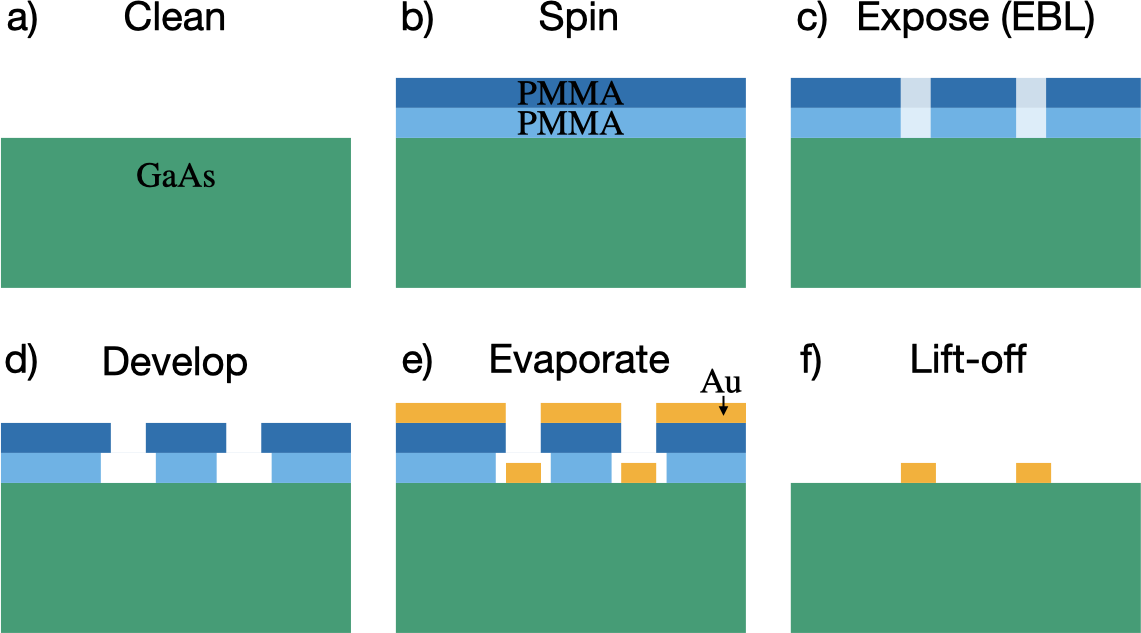
\includegraphics[width=1.0\textwidth]{figures/appendix/crop_FiguresMaster.020.png}
    \caption[Step by step illustration for fabricating metal gates]{\label{fig:appx/gate_fab} 
    (\textbf{a}) GaAs/AlGaAs heterostructure is cleaned in an Ultra Sonic (US) bath with acetone/IPA/DI. 
    (\textbf{b}) Two different layers of PMMA are spun ontop of the heterostructure.
    (\textbf{c}) The gate design is exposed to an electron beam to breakup the PMMA.
    (\textbf{d}) The chip is developed in an IPA:DI solution create an undercut and remove the exposed PMMA.
    (\textbf{e}) 2:\qty{12}{nm} of Ti:Au are evaporated ontop of the chip.
    (\textbf{f}) The chip is rinsed in acetone to remove remaining PMMA and any metal attached to it. The chip is ready to be placed onto a chip carrier, wirebonded and measured.}
  \end{center}
\end{figure}



\subsubsection{Outer gates and bondpads }

\begin{enumerate}
\item Solvent clean – Acetone, IPA. Rinse in DI, blow dry with $\mathrm{N_22}$.
\item Prebake chip for $3\,\mathrm{minutes}$ at $180^\circ$C.
\item Spin PMMA A8 495K at $4000\,\mathrm{RPM}$ for $40\,\mathrm{s}$  with $3\,\mathrm{minutes}$ bake at $180^\circ$C
\item Spin PMMA A4 490K at $4000\,\mathrm{RPM}$ for $40\,\mathrm{s}$  with $5\,\mathrm{minutes}$ bake at $180^\circ$C
\item E beam lithography in Jeol JBX 8100FS : Dose \qty{1100}{\mu C/cm^2}
\item Develop in IPA:DI, 7:3 $40\,\mathrm{s}$ at $18^\circ$C, stop in DI.
\item $\mathrm{O_2}$ plasma etch in Plasma etch PE 50, $1\,\mathrm{minutes}$.
\item Evaporate Ti $10\,\mathrm{nm}$, $2\,\mathrm{\dot{A}s^{-1}}$ then Au $100\,\mathrm{nm}$, $4\,\mathrm{\dot{A}s^{-1}}$.
\item Liftoff in Acetone at room temperature.
\end{enumerate}




\subsection{Wire Bonding}

The final step in the fabrication process is to attach the chip to a chip carrier and connect the gates and ohmics to bond pads. The chip carrier is added to the fridge and connected to the fridge wiring which lead to a break out box outside the fridge. 


\begin{enumerate}
\item Stick the chip to the chip carrier using a small dab of PMMA A8 495K. Bake for $5\,\mathrm{minutes}$ at $60^\circ$C
\item Wirebond bond pads on chip carrier to gates and ohmics on the chip:
\begin{table}[H]     
\centering
  \begin{tabular}{|p{3.0cm}|p{2.0cm}|p{2.0cm}|}
    \hline
     & Bond 1 & Bond 2\\
    \hline
    Wire material & Al & Al\\
    Bond strength & 260 & 300\\
    Bond duration & \qty{30}{ms} & \qty{30}{ms} \\
    \hline
  \end{tabular}
\label{tab:wire_bonding}
\end{table}
\end{enumerate}

% \chapter{First Appendix}
% Here you can have your appendices.  Note that if you only have a
% single appendix, you should issue
% \verb|\renewcommand{\appendicesname}{Appendix}| before calling
% \verb|\appendix| to display the singular ``Appendix'' rather than the
% default plural ``Appendices''.

\chapter{Second Appendix}
Here is the second appendix.

%% This changes the headings and chapter titles (no numbers for
%% example).
\backmatter



\end{document}
\endinput
%%
%% End of file `ubcsample.tex'.
